% Magic Comments
% !TeX spellcheck = en_GB
% !TeX encoding = utf8
% !TeX program = pdflatex

\documentclass[12pt, oneside]{amsart}

\usepackage{amssymb}
\usepackage[
style=numeric-comp,
backend=biber,
sorting=nty,
doi=false,
isbn=false, 
natbib=true]{biblatex}
\addbibresource{references.bib}
\emergencystretch=1em

\usepackage{mathtools}
\usepackage{xcolor}
\usepackage{url} % Makes urls nicer
\usepackage[breaklinks=true]{hyperref}
\usepackage{cleveref}

% For tabular
\usepackage{booktabs}
\usepackage{array}
\usepackage{adjustbox}
\usepackage{multirow}
\usepackage{makecell}

% For figures
\usepackage{graphicx}

% Floating for positioning environments
\usepackage{float}


\newtheorem{thm}{Theorem}[section]
\newtheorem{prop}[thm]{Proposition}
\newtheorem{lem}[thm]{Lemma}
\newtheorem{cor}[thm]{Corollary}

\theoremstyle{definition}
\newtheorem{definition}[thm]{Definition}

\theoremstyle{remark}
\newtheorem{remark}[thm]{Remark}

\numberwithin{equation}{section}


% Package specific things

% TODO: Do we want to have equations just labeled with "(3.1)" or with 
% TODO: "equation 3.1".
%\crefname{equation}{equation}{equations} 
%\Crefname{equation}{Equation}{Equations}
\crefname{equation}{}{} 
\Crefname{equation}{}{}

\crefname{table}{table}{tables}
\Crefname{table}{Table}{Tables}

\crefname{figure}{figure}{figures}
\Crefname{figure}{Figure}{Figures}


% Definitions
\newcommand{\defn}{\ensuremath{:=}}
\newcommand{\revdefn}{=:}

% Sets
\newcommand{\R}{\mathbb{R}}
\newcommand{\N}{\mathbb{N}}
\newcommand{\Z}{\mathbb{Z}}
\newcommand{\C}{\mathbb{C}}
\newcommand{\Q}{\mathbb{Q}}
\newcommand{\T}{\mathbb{T}}

% Caligraphic
\newcommand{\cO}{\mathcal{O}}
\newcommand{\cZ}{\mathcal{Z}}
\newcommand{\cP}{\mathcal{P}}
\newcommand{\cI}{\mathcal{I}}
\newcommand{\cA}{\mathcal{A}}

% Function Spaces
\newcommand*{\pols}[2][]{\ensuremath{\cP^{#1}\left(#2\right)}}

% bold
\newcommand{\ZZ}{\ensuremath{\mathbf{Z}}}
\newcommand{\FF}{\ensuremath{\mathbf{F}}}
\newcommand{\XX}{\ensuremath{\mathbf{X}}}

% Set brackets
\newcommand{\set}[1]{\left\{#1\right\}}

% Make index set from 1 to (inclusive) m:
\newcommand*{\indexset}[2][1]{[#1:#2]}

% Make a colon: (Used for defining a function from A to B)
\newcommand*{\from}{\colon}

% Probability commands: Expectation, Variance, Covariance, Bias
\newcommand{\E}{\mathbb{E}}

% Vector Norm
\newcommand{\norm}[2][2]{\left\lVert#2\right\rVert_{#1}}

% Derivatives
\newcommand{\deriv}[2][x]{\frac{\mathrm{d}}{\mathrm{d}#1} (#2)}

% Partial derivatives
\newcommand{\pderiv}[2]{\frac{\partial #1}{\partial #2}}

% Integral 
\newcommand{\integral}[4]{\int\limits_{#1}^{#2}#3~\mathrm{d}#4}

% Inner product
\newcommand{\inner}[2]{\left\langle#1,#2\right\rangle}

% Absolute value
\newcommand{\abs}[1]{\left \vert #1 \right \vert }

% If else (ternary operator)
\newcommand{\ifelse}[3]{#1~\textrm{if}~#2~\textrm{else}~#3}

% Vector-Arrow
\newcommand{\vecarrow}[1]{\vec{#1}}

% Vector 2 dimensions
\newcommand{\vtwo}[2]{\left(\begin{array}{c}#1\\#2\end{array}\right)}

% Vector 3 dimensions
\newcommand{\vthree}[3]{\left(\begin{array}{c}#1\\#2\\#3\end{array}\right)}

% Large Limit bar for defined integral borders
\newcommand{\eval}[2]{\Biggr|_{#1}^{#2}}

% Divides symbol
\newcommand{\divides}{\vert}

% Changing greek letters
\let\uglyepsilon\epsilon % Still saving the previous one
\let\epsilon\varepsilon

\let\otherphi\phi % Still saving the previous one
\let\phi\varphi

% Images from inkscape

\newcommand{\incfig}[2][\columnwidth]{%
	\def\svgwidth{#1}
	\import{../figures/}{#2.pdf_tex}
}

\renewcommand*{\aa}{\mathbf{a}}

\renewcommand*{\Re}{\mathrm{Re}}
\renewcommand*{\Im}{\mathrm{Im}}

%Shortcuts
\renewcommand{\d}{\mathrm{d}}

% Mathematical Operators:
\DeclareMathOperator*{\supp}{supp} % support of a vector
\DeclareMathOperator*{\argmin}{argmin}
\DeclareMathOperator*{\spn}{span}
\DeclareMathOperator{\id}{id}
\DeclarePairedDelimiter\ceil{\lceil}{\rceil}
\DeclarePairedDelimiter\floor{\lfloor}{\rfloor}

% For tabulars
\newcommand{\first}[1]{\textbf{#1}}

% Quotation marks
\newcommand*{\quotes}[1]{``#1''}


% Comments
\newcommand*{\jakob}[1]{\color{red} \textbf{\emph{#1}} \color{black}}
\newcommand*{\elias}[1]{\color{blue} \textbf{\emph{#1}} \color{black}}
\newcommand*{\mario}[1]{\color{green} \textbf{\emph{#1}} \color{black}}

% %%%%%%%%%%%%%%%%%%%%%%%%%%%%%%%%%%%%%%%%%%%%%%%%%%%%%%%%%%%%%%%%% %

% TODO: Use geometry package to have more space?
% TODO: Tables' size can be increased when setting the width in the adjustbox

\begin{document}
\title{Least Squares and Smolyak's Algorithm}


\author{Jakob Eggl, Elias Mindlberger and Mario Ullrich}
\date{\today}
\keywords{Polynomial interpolation, Sparse-Grids, Least-Squares, Smolyak} % 

%\author{Jakob Eggl}
%\address{Institute of Analysis, Johannes Kepler University Linz, Austria.}
%\email{jakob.eggl@jku.at}
%
%\author{Elias Mindlberger}
%\address{Institute of Analysis, Johannes Kepler University Linz, Austria.}
%\email{elias.mindlberger@jku.at}
%
%\author{Mario Ullrich}
%\address{Institute of Analysis, Johannes Kepler University Linz, Austria.}
%\email{mario.ullrich@jku.at}

% \thanks{\(\star\) Equal Contribution.}


\begin{abstract}
	We present novel, large-scale experiments for polynomial interpolation in 
	high 
	dimensional settings using some of the most popular algorithms available. 
	We 
	compare Smolyak's Algorithm (SA) on sparse grids and Least Squares (LSQ) 
	using 
	random data. We empirically confirm that interpolation using LSQ performs 
	equally as good on smooth and better on non-smooth functions if SA is given 
	\(n\) and LSQ is given \(2 \cdot n\) points.
\end{abstract}

\maketitle

%\tableofcontents

%%%%%%%%%%%%%%%%%%%%%%%%%%%%%%%%%%%%%%%%%%%%%%%%%%%%%%%%%%%
\section{Introduction}
%%%%%%%%%%%%%%%%%%%%%%%%%%%%%%%%%%%%%%%%%%%%%%%%%%%%%%%%%%%

Smolyak's algorithm on Sparse Grids has been of high theoretical and practical 
interest for a long time 
\cite{BarthelmannHighDim_2000,smolyak1963,Coleman_SmoylakGithub_2013,JuddSmolyak_2014}.
 In \cite{Krieg_2020}, it was recently found that Smolyak's algorithm is 
\emph{not} optimal in the sampling numbers
\[
e_n(H) \defn \inf_{\substack{x_1, \dots, x_n \in D \\ \phi_1, \dots, \phi_n 
		\in L_2}} \sup_{f \in B(H)} \norm[L_2]{f - \sum_{i=1}^n f(x_i) \phi_i}
\]
disproving conjecture 5.26 in \cite{Dung_Temlyakov_Ullrich_2018}. We extend 
upon these theoretical findings with an empirical study comparing the 
performance of Smolyak's algorithm and Least Squares on simple function 
recovery problems on the unit cube. Our implementation is available at 
\url{https://github.com/th3lias/NumericalExperiments}.


%%%%%%%%%%%%%%%%%%%%%%%%%%%%%%%%%%%%%%%%%%%%%%%%%%%%%%%%%%%
\section{Notation}
%%%%%%%%%%%%%%%%%%%%%%%%%%%%%%%%%%%%%%%%%%%%%%%%%%%%%%%%%%%

We denote the indexset containing all indices $i\in \Z$ 
where $m\leq i\leq n$ for $m\leq n$ with \(\indexset[m]{n}\). For the set of 
polynomials \(p\) from \(D \subseteq \C^K,\, K \in \N\) to the field \(\F\) of F
maximal 
degree \(N\) we use the notation 
\(p \in \pols[N]{V, \F}\).
We use \(f \lesssim g\) to denote \(f \leq c 
g\) for functions \(f, g\). With \(B(X)\) we denote the closed unit ball of a 
normed space \(X\). With \(X^\star\) we denote the topological dual space of 
\(X\).
\newpage
%%%%%%%%%%%%%%%%%%%%%%%%%%%%%%%%%%%%%%%%%%%%%%%%%%%%%%%%%%%
\section{Interpolation}
%%%%%%%%%%%%%%%%%%%%%%%%%%%%%%%%%%%%%%%%%%%%%%%%%%%%%%%%%%%

Given \(i \in \N\) and distinct data points \(\XX_i \defn \set{x_{i, 0}, \dots, 
	x_{i, n}} \subseteq D_i \subseteq \R\), function values 
\(\YY_i \defn \set{y_{i, 0}, \dots, y_{i, n}} = \set{f(x_{i, 0}), \dots, 
	f(x_{i, n})} \subseteq \R\) for \(f: D_i \to \R\), it is a well known fact 
	that 
there exists a polynomial \(\cI(\ZZ_i)\) of degree \(n\) such that \[
\cI(\ZZ_i) = y_{i, j},\quad j \in \indexset[0]{n}.
\]
for \(\ZZ_i \defn (\XX_i, \YY_i)\)
We then call \(\cI(\ZZ_i)\) an \emph{interpolating} polynomial. It can be 
written down explicitly as \begin{equation}\label{interpolating_polynomial}
	\cI(\ZZ_i) = \sum_{j=0}^n y_{i, j} \ell_{i, j}
\end{equation}
for basis functions \(\ell_{i, j} \in \pols[n]{\R, \R}\). Moreover, in a single 
dimension, the formula for this basis is
\[
\ell_{i, j}(w) = \prod_{m \in \indexset[0]{n} \setminus \set{j}} \frac{w-x_{i, 
		m}}{x_{i, j}-x_{i, m}},
\]
see \cite{waring1779, lagrange1901}. We call \(\cI\) the 
\emph{Lagrange interpolator}.

Suppose now we have \(d\) point sets \(\XX_i\). By taking the full cartesian 
product of point sets \[
\XX \defn \bigtimes_{i=1}^d \XX_i,
\] we may identify our grid by \(\XX = \set{\bfx_\bfj}_{\bfj}\) with \(\bfj \in 
\set{0,1,\dots,n}^d\) and suppose we have according function evaluations \(\YY 
\defn \set{y_\bfj}_\bfj = \set{f(\bfx_\bfj)}_\bfj\) for \(f: D \to \R\), \(D 
\subseteq \R^d\). Let \(\ZZ \defn (\XX, \YY)\). Then, we may construct an 
interpolating polynomial as in \cref{interpolating_polynomial}. Indeed, the 
general formula stays the same but we take tensor product of basis functions, 
i.e. \begin{equation}\label{multivariateLagrange}
	\ell_\bfj(\bfw) = \bigotimes_{i=1}^d \ell_{j_i}(w_i) = \prod_{i=1}^d 
	\ell_{j_i}(w_i) = \prod_{i=1}^d \prod_{\substack{k=0 \\ k \neq j_i}}^n 
	\frac{w_i - x_{i, k}}{x_{i, j_i} - x_{i, k}}
\end{equation}
and the sum now ranges over all multiindices \(\bfj = (j_1, \dots, j_d) \in 
\N_0^d\) with \(\bfj \in \set{0, 1, \dots, n}^d\). We denote 
\begin{equation}\label{eq:interpolantdD}
	\cI(\ZZ) \defn \sum_{j_1 = 0}^n \cdots \sum_{j_d = 0}^n y_{j_1, \dots, j_d} 
	\ell_{j_1, \dots, j_d}
\end{equation}
for the interpolant on \(\R^d\).
Formula \ref{multivariateLagrange} is not a great choice for performing 
calculations on hardware. Leaving the storage of \((n+1)^d\) grid points aside, 
for computing one evaluation of the map \(\bfw \mapsto \cI(\ZZ)(\bfw)\), one 
must compute the sum of \((n+1)^d\) terms, where in each summand, the 
evaluation of \(d\) basis functions is computed, each of which is a product of 
\(n\) terms. This evaluation is thus as costly as \(\cO((n+1)^d d n)\). One can 
counter the costly computation of the interpolating polynomial at a given point 
by reformulating the above (numerically instable) Lagrange interpolator in it's 
barycentric form
\begin{equation}\label{eq:multivarBarycentric}
	\cI(\ZZ)(\bfw) = \frac{\sum_{j_1=0}^{n} \ell^{(1)}_{j_1}(w_1) \cdots 
	\sum_{j_d=0}^{n} \ell^{(d)}_{j_d}(w_d) y_\bfj}{\sum_{j_1=0}^{n} 
	\ell^{(1)}_{j_1}(w_1) \cdots \sum_{j_d=0}^{n} \ell^{(d)}_{j_d}(w_d)}
\end{equation}
where
\begin{equation}\label{eq:barycentricBasis}
	\ell^{(k)}_{j_k}(w) \defn \frac{m_{j_k}}{w-x_{j_k}} \mid k \in 
	\indexset[1]{d}.
\end{equation}
with \(x_{j_k}\) being the \(j_k\)--th entry of \(\bfx\). \(m_{j_k}\) are the 
\emph{barycentric} weights which can be computed in \(\cO(n^2)\) time for 
general point distributions but admit \(\cO(1)\) computation for well--known 
and widely used point sets \cite{klimke2004}. For example, due to 
\cite{Berut_2004},
\begin{equation}\label{barycentric_weights_chebyshev}
	m_{0} = \frac{1}{2},\quad m_{l} = (-1)^l,\, l \in \indexset[1]{n-1},\quad 
	m_n = \frac{1}{2}(-1)^n
\end{equation}
for the \emph{Chebyshev Gauss-Lobatto} (or just Chebyshev extrema), in which 
\begin{equation}\label{ChebyshevGaussLobatto}
	x_l \defn x_{l,n} \defn - \cos\frac{l \pi}{n},\, l \in \indexset[0]{n}.
\end{equation}

Similarly, for the \emph{Chebyshev points of the second kind}
\begin{equation}\label{eq:chebyPts2}
	x_l = x_{l, n} = \cos \frac{l \pi}{n},\, l \in \indexset[0]{n}
\end{equation}
one gets the closed form
\begin{equation}\label{eq:weightsChebyshev}
	m_l = {\left(-1\right)}^l \cdot \begin{cases}
		1/2 &l \in \set{0, n}\\
		1 &\text{else.}
	\end{cases}
\end{equation}
In this case, one achieves an evaluation time of \(\cO((n+1)^d)\).
Hence, in this construction, one cannot get around this bottleneck. 
\jakob{Here, equation \cref{eq:chebyPts2} and \cref{eq:weightsChebyshev} are 
	the same point set. This is probably wrong.}


%%%%%%%%%%%%%%%%%%%%%%%%%%%%%%%%%%%%%%%%%%%%%%%%%%%%%%%%%%%
\section{Smolyak's Algorithm \& Sparse Grids}
%%%%%%%%%%%%%%%%%%%%%%%%%%%%%%%%%%%%%%%%%%%%%%%%%%%%%%%%%%%

The following description follows \cite{BarthelmannHighDim_2000}.
The question arises, how one may reduce the complexity of exact interpolation 
on grids. The central idea of sparse grids is to \emph{not} take the full 
tensor product of one dimensional point sets but restrict the number of 
simultaneously large directions. To that end, take a variable 
number of points in each direction, i.e.\ let \(\XX_j \defn \set{x_{1, j}, 
	\dots, x_{N(j), j}}\) and \(\cI_j\) the corresponding one--dimensional 
interpolator with \(\cI_0 \defn 0\), \(\Delta_j \defn \cI_j - \cI_{j-1}\). Then 
Smolyak's algorithm is given in a simple recursive manner
\begin{equation}\label{Smolyak}
	\cA(q, d) \defn \sum_{\norm[1]{\bfj} \leq q} \bigotimes_{k=1}^d 
	\Delta_{j_k} = \cA(q-1, d)+\sum_{\norm[1]{\bfj}=q} \bigotimes_{k=1}^d 
	\Delta_{j_k}
\end{equation}
with \(\cA(q, d) = 0,\, q < d\) and \(\bfj\), \(\cI\) as before. Evidently, 
only a relatively small number of knots, through the restriction 
\(\norm[1]{\bfj} \leq q\), is needed. To be precise, \(\cO(n (\log n)^{d-1})\) 
points are needed. Hence \(q\) can be thought of as a resolution parameter. By 
this form, one only needs to assess the function values at the \emph{sparse 
grid} \[
H(q, d) \defn \bigcup_{q-d+1 \leq \norm[1]{\bfj} \leq q} \XX_{j_1} \times 
\cdots \times \XX_{j_d}
\]
where the number of nodes in a given direction can never be \emph{large} for 
all directions simultaneously. Hence, given that \(\XX_j \subset \XX_{j+1}\), 
one may write the interpolator given by Smolyak's construction as \[
\cA(q, d)(f) = \sum_{\norm[1]{\bfj} \leq q} f(\bfx_\bfj) \ell_\bfj,
\]
which is familiar from before.
The number of knots \(N(j)\) used for each one--dimensional interpolation rule 
\(\cI_j\) remains to be specified. In order to obtain nested points, i.e. 
\(\XX_j \subset \XX_{j+1}\) and thus \(H(q, d) \subset H(q+1,d)\) together with 
collocation rules such as \cref{ChebyshevGaussLobatto} or \cref{eq:chebyPts2} 
it is usual to choose a doubling rule, i.e. \[
N(1) = 1,\quad N(j) = 2^{j-1}+1,\, j > 1.
\]

\subsection{Polynomial Exactness}
Without loss of generality, we restrict ourselves to the symmetric cube \([-1, 
1]^d\) \jakob{We have $[0,1]^d$. It appears multiple times, therefore I didn't 
	want to erase it everywhere now.} for interpolation of unknowns instead of 
	a 
general domain \(D\). In this 
case, Smolyak's algorithm is well known to exactly reproduce functions on 
certain polynomial spaces given that the rules \(\cI_j\) are exact on nested 
spaces \(V_j\), see \cite{DELVOS198299} or \cite{novakRitter1996}.
\begin{lem}
	Assume \(\cI_j\) is exact on the vector space \(V_j \subseteq C([-1, 1])\) 
	and assume \[
	V_1 \subset V_2 \subset V_3 \subset \dots,
	\]
	then \(\cA(q, d)\) is exact on \[
	\sum_{\norm[1]{j}=q} V_{j_1} \otimes \cdots \otimes V_{j_d}
	\]
\end{lem}
\cite{BarthelmannHighDim_2000} showed the following. \jakob{Maybe cite 
	\cite{BarthelmannHighDim_2000} directly in the lemma environment. I.e. 
	begin{lem}[cf. \cite{BarthelmannHighDim_2000}]}
\begin{lem}
	\(\cA(q, d)\) is exact on \[
	E(q, d) \defn \sum_{\norm[1]{\bfj} = q} \pols[m_{j_1}-1]{\R, \R} \otimes 
	\cdots \otimes \pols[m_{j_d}-1]{\R, \R}
	\]
	and \(\cA(d+k, d)\) is exact for all polynomials of degree \(k\).
\end{lem}
Indeed, the following also follows from \cite{BarthelmannHighDim_2000}. Note 
that we now abuse the notation from \ref{interpolating_polynomial} by writing 
\(\cI(\ZZ) \revdefn \cI(f, \XX) \revdefn \cI(f)\).
\begin{lem}
	Assume \(\XX_1 \subset \XX_2 \subset \dots\) and \(\cI_j(f)(x) = f(x)\) for 
	every \(f \in C([-1, 1])\) and every \(x \in \XX_j\). Then \[
	\cA(q, d)(f)(x) = f(x)
	\]
	for every \(f \in C([-1, 1]^d)\) and \(x \in H(q, d)\).
\end{lem}

\subsection{Error Bounds}
Since the interpolation operator \(\cI_j\) as defined before is exact on 
\(\pols[N(j)-1]{\R, \R}\) one concludes \[
\norm[\infty]{f - \cI_j(f)} \leq \err_{N(j)-1}(f)(1+\Lambda_{N(j)})
\]
where \(\err_n\) is the error of the best approximation by \(p \in \pols[n]{\R, 
\R}\), \(\Lambda_n\) is the Lebesgue constant for the point set in 
\Cref{ChebyshevGaussLobatto} and \(n \geq 2\), in which case it is known that \[
\Lambda_n \leq \frac{2}{\pi} \log(n-1)+1,
\]
see for example \cite{zeller1966} and \cite{Dzjadyk1983}. The following bounds 
can be found in \cite{BarthelmannHighDim_2000} and is well known since 
\cite{smolyak1963, temlyakov1986, WASILKOWSKI19951}.

\begin{lem}
	For the space
	\[
	F_d^k \defn \set{f: [-1, 1]^d \to \R \mid D^\alpha f \text{ continuous if } 
	\alpha_i \leq k \text{ for all } i}
	\]
	the error of \(\cA(q, d)\) can be bounded as \[
	\norm[\op]{I_d - \cA(q, d)} \leq c_{d,k} n^{-k} \left(\log 
	n\right)^{(k+2)(d-1)+1}
	\]
	where \(I_d\) is the embedding \(F_d^k \hookrightarrow C([-1, 1]^d)\) and 
	\(c_{d, k}\) is a positive constant only dependent on \(d\) and \(k\).
\end{lem}

Moreover, for the Sobolev--Hilbert space \(H_w^k\) with \begin{equation}
	H_w^k \defn \set{f \in L^2_w : \norm[k]{f}^2 = \sum_{\ell \in \N_0} 
	(1+\ell^2)^k \inner{f}{b_\ell}^2 < \infty}
\end{equation}
with \(\inner{f}{b_\ell}\) being the \(\ell\)--th Fourier coefficient, one 
obtains \[
\norm[0]{f-\cA(q, d)(f)} \leq c_{d, k} n^{-k} \left(\log 
n\right)^{(k+1)(d-1)}\norm[k]{f}.
\]
Here, \(L^2_w\) is the \(L^2\) weighted by the Chebyshev weight 
\begin{equation}\label{chebyshev_weight}
	\left(1-x^2\right)^{-1/2}.
\end{equation}
In that case, it is well known that the Chebyshev polynomials
\begin{equation}\label{chebyshev_polynomials}
	T_n(x) \defn \cos(n \arccos(x)).
\end{equation}
form an orthonormal basis.

%%%%%%%%%%%%%%%%%%%%%%%%%%%%%%%%%%%%%%%%%%%%%%%%%%%%%%%%%%%
\section{Least Squares}
%%%%%%%%%%%%%%%%%%%%%%%%%%%%%%%%%%%%%%%%%%%%%%%%%%%%%%%%%%%

Contrary to the construction of exactly interpolating approximants in the case 
of Smolyak's algorithm, Least Squares is a conceptually simpler algorithm. We 
are given the overdetermined system \[
A\bfz = \bfy
\]
where \(A \in \R^{n \times m}\) with \(n > m\). It is well--known that this 
system may be inconsistent and no exact solution exists. However, one may 
always pose the optimisation problem solving for \(\bfz \in \R^{m}\) with the 
smallest error
\begin{equation}\label{eq:leastSquares}
	\inf_{\bfz \in \R^{m}} \norm[]{A\bfz - \bfy}.
\end{equation}
It is further known that, in case of a full--rank matrix \(V\), the unique 
solution to \Cref{eq:leastSquares} is given by 
\begin{equation}\label{eq:ls_solution_moore_penrose_inverse}
	\bfz_* = \left(A^\top A\right)^{-1} A^\top \bfy \in \R^m.
\end{equation}
In our specific case of polynomial interpolation, \(A\) is the Vandermonde 
matrix, consisting of basis polynomials \(b_1, b_2, \dots, b_m\) evaluated at 
the $n$ different sampled points \(x_1, x_2, \dots, x_n\) in \(D \subseteq 
\R^d\) and \(\bfy\) is the vector of function values sampled from the unknown 
function \(f\from D \to \R\), i.e.\ \(\bfy = \left(f(\bfx_j)\right)_{j=1}^n\). 
As for such points, the Vandermonde matrix is never singular, the solution to 
the approximation problem \[
\inf_{p} \norm[]{f-p}
\]
can analytically be expressed as \[
p_* \from D \to \R,\quad t \mapsto \sum_{j=1}^m z_{*_{j}} b_j(t)
\]
where \(\bfz_* = \left(z_{*_j}\right)_{j=1}^m\) is given by 
\Cref{eq:ls_solution_moore_penrose_inverse}.
For the later implementation, we choose the basis polynomials \(b_j\) as the 
\(j\)--th weighted Chebyshev polynomial \Cref{chebyshev_polynomials}.

%%%%%%%%%%%%%%%%%%%%%%%%%%%%%%%%%%%%%%%%%%%%%%%%%%%%%%%%%%%
\section{Theoretical Guarantees}
%%%%%%%%%%%%%%%%%%%%%%%%%%%%%%%%%%%%%%%%%%%%%%%%%%%%%%%%%%%

% TODO: Eventuell diesen Abschnitt an ein Banachraum Setting anpassen, wie in 
%https://arxiv.org/pdf/2401.02220.

The notation in the following is borrowed from \cite{Ullrich_2020}.
In this section we introduce a formal setting to the former considerations. 
That is, we consider a Hilbert space \(H\) of real-valued functions on a set 
\(D\) such that point evaluation \(\delta_x: f \mapsto \int_D f\ \d \delta_x = 
f(x)\)
is a bounded, linear functional on \(H\).
The general formulation of Least Squares allows for a broad class of recovery 
problems. In our specific case, the function recovery of real--valued functions 
on a \(d\)--dimensional (compact) subset \(D\) using basis functions of a 
\(k\)--dimensional subspace \(V_k \defn \spn \set{b_1, \dots, b_k}\), we 
consider the specific form of Least Squares, given by\[
A_{n, k}(f) \defn \argmin_{g \in V_k} \sum_{i=1}^n \frac{\abs{g(x_i) - 
f(x_i)}^2}{\varrho_k(x_i)}
\]
where \[
\varrho_k(x) = \frac{1}{2} \left( \frac{1}{k} \sum_{j < k} b_{j+1}(x)^2 + 
\frac{1}{\sum_{j \geq k} a_j^2} \sum_{j \geq k} a_j^2 b_{j+1}(x)^2 \right)
\]
and \(x_1, \dots, x_n \in D\). Whenever \(f \in V_k\), then, of course, \(f = 
A_{n, k}(f)\). With
\begin{equation}\label{eq:worstCaseError}
	e\left(A_{n,k}, H\right) \defn \sup_{f \in B(H)} \norm[L_2]{f - A_{n,k}(f)},
\end{equation}
we denote the worst case error of \(A_{n,k}\), where we measure the error of 
the reconstruction in the space \(L_2 \defn L_2(D, \Sigma, \mu)\) of square 
integrable functions on \(D\) with respect to the measure \(\mu\), such that 
\(H\) is embedded into \(L_2\). In light of this, the \(n\)--th minimal error 
(also called \(n\)--th sampling number) is denoted by \[
e_n(H) \defn \inf_{\substack{x_1, \dots, x_n \in D \\ \phi_1, \dots, \phi_n 
		\in L_2}} \sup_{f \in B(H)} \norm[L_2]{f - \sum_{i=1}^n f(x_i) \phi_i}
\]
and can be understood as the worst case error of the optimal algorithm using 
\(n\) function values. We get the clear inequality \(e_n(H) \leq e(A_{n,k}, 
H)\) for any point set \(\set{x_1, \dots, x_n}\). With \[
a_n(H) \defn \inf_{\substack{h_1^\star, \dots, h_n^\star \in H^\star \\ 
		\phi_1, \dots, \phi_n \in L_2}} \sup_{f \in B(H)} \norm[L_2]{f - 
	\sum_{i=1}^n h_i^\star(f) \phi_i}
\]
we denote the \(n\)-th approximation number, which is the worst-case error of 
an optimal algorithm that uses the \(n\) best arbitrary linear and bounded 
functionals as information about the unknown. This quantity is equal to the 
\(n\)-th singular value of the embedding \(\id\from H \to L_2\).

The following is known since \cite{Krieg_2020}.
\begin{thm}[Krieg--Ullrich]\label{thm:kriegUllrich2020}
	There exist constants \(C, c > 0\) and a sequence of natural numbers 
	\((k_n)\) with each \(k_n \geq cn/\log(n+1)\) and for any \(n \in \N\) and 
	measure space \((D, \Sigma, \mu)\), and any RKHS \(H\) of real-valued 
	functions on \(D\) embedded into \(L_2(D, \Sigma, \mu)\), we have \[
	e_n(H) \leq \sqrt{\frac{C}{k_n} \sum_{j \geq k_n} a_j(H)^2}.
	\]
\end{thm}
In particular, for 
\begin{equation}\label{eq:orderOfApproximationNumbers}
	a_n(H) \lesssim n^{-s} \log^{\alpha + s}(n)
\end{equation}
with \(s > 1/2, \alpha \in \R\), this implies \[
e_n(H) \lesssim n^{-s} \log^{\alpha+s}(n).
\]
The following follows from \cite{Ullrich_2020}.
\begin{thm}[Ullrich]
	Given \(n \geq 2\) and \(c > 0\), let \[
	k_n \defn \floor*{\frac{n}{2^8 (2+c) \log n}},
	\]
	then, for any measure space \((D, \Sigma, \mu)\) and any RKHS \(H\) of 
	real-valued functions on \(D\), embedded into \(L_2(D, \Sigma, \mu)\), it 
	holds that \[
	e_n\left(A_{n, 2 k_n}, H\right) \leq \sqrt{ \frac{2}{k_n} \sum_{j > k_n} 
	a_j(H)^2 }
	\]
	with probability at least \(1-8n^{-c}\).
\end{thm}

\subsection*{Examples}
In particular, \Cref{eq:orderOfApproximationNumbers} is satisfied for the 
approximation numbers on the Sobolev space of dominating mixed smoothness, 
\begin{align*}
	H &\defn H_{\text{mix}}^s\left(\T^d\right)\\
	&\defn \set{f \in L_2\left(\T^d\right) : \norm[H]{f}^2 \defn \sum_{m \in 
			\N_0^d} \prod_{j=1}^d (1+\abs{m_j}^{2s}) \inner{f}{b_m}^2_{L_2} < 
			\infty}
\end{align*}
with \(\T^d \cong [0, 1)^d\) 
where \(b_m \defn \otimes_{j=1}^d b_{m_j}^{(1)}\) and \(m = (m_1, \dots, m_d)\) 
with \begin{align*}
	b_{2m}^{(1)} &\defn \sqrt{2}\cos(2\pi m x)\\
	b_{2m-1}^{(1)} &\defn \sqrt{2}\sin(2\pi m x)
\end{align*}
and \(b_0^{(1)} \defn 1\). This satisfies the assumption for \(s > 1/2\). In 
particular, we can say
\begin{equation}\label{eq:conclusio}
	e_n\left( H_{\text{mix}}^s\left(\T^d\right) \right) \lesssim 
	n^{-s}\log^{sd}(n)
\end{equation}
whenever \(s > 1/2\). This disproves a previously posted conjecture (Conjecture 
5.26) in \cite{Dung_Temlyakov_Ullrich_2018} and shows that Smolyak's algorithm 
is not optimal in this case. The surprising fact is that, despite an optimal, 
deterministic construction of the point sets used for reconstruction being 
unknown, random i.i.d. points suffice for a reconstruction error that is on the 
order of optimal points, with probability tending to \(1\). We verify this by 
our experimental findings, presented in \Cref{sec:experimentalFindings} with a 
much better relative number of points used for LSQ function recovery vs. SA 
recovery than guaranteed in this section, i.e. better constants than explicitly 
known before. It remains an open problem to rigorously improve upon the 
constants in \Cref{eq:conclusio}.
%%%%%%%%%%%%%%%%%%%%%%%%%%%%%%%%%%%%%%%%%%%%%%%%%%%%%%%%%%%
\section{Experimental Findings}\label{sec:experimentalFindings}
%%%%%%%%%%%%%%%%%%%%%%%%%%%%%%%%%%%%%%%%%%%%%%%%%%%%%%%%%%%

% TODO: Add what computer and software we used etc. Also how much RAM was used
% TODO: And also, how long it took.

For assessing the performance of the Least Squares algorithms in comparison to 
the Sparse Grid alternative, we use the following $12$ families of test 
functions from \cite{Simulationlib_2013}, each defined of the $d$-dimensional 
unit-cube $[0,1]^d$.

{
	\allowdisplaybreaks[4]
	\begin{align*}
		\begin{array}{l l}
			\text{1. Continuous:} & f_1(x) = \exp\left( - 
			\sum_{i=1}^{d} c_i \abs{x_i - w_i} \right) \\[12pt]
			\text{2. Corner Peak:} & f_2(x) = \left( 1 + 
			\sum_{i=1}^{d} c_i x_i 
			\right)^{-(d+1)} \\[12pt]
			\text{3. Discontinuous:} & f_3(x) = 
			\begin{cases}
				0, &x_1 > w_1 \lor x_2 > w_2, \\
				\exp\left( \sum_{i=1}^{d} c_i x_i \right), & 
				\text{else}
			\end{cases} \\[12pt]
			\text{4. Gaussian:} & f_4(x) = \exp\left( - 
			\sum_{i=1}^{d} c_i^2 (x_i 
			- w_i)^2 \right) \\[12pt]
			\text{5. Oscillatory:} & f_5(x) = \cos\left( 2\pi w_1 + 
			\sum_{i=1}^{d} c_i x_i \right) \\[12pt]
			\text{6. Product Peak:} & f_6(x) = \prod_{i=1}^{d} 
			\left( c_i^{-2} + (x_i - w_i)^2 \right)^{-1} \\[12pt]
			\text{7. G-Function:} & f_7(x) = \prod_{i=1}^{d}
			\frac{\abs{4x_i-2-w_i}+c_i}{1+c_i}
			\\[12pt]
			\text{8. Morokoff \& Calfisch 1:} & f_8(x) = 
			\left(1+1/d\right)^d  
			\prod_{i=1}^{d}\left(c_ix_i+w_i\right)^{1/d}
			\\[12pt]
			\text{9. Morokoff \& Calfisch 2:} & f_9(x) = 
			\frac{1}{\left(d-0.5\right)^d} 
			\prod_{i=1}^{d}\left(d-c_ix_i+w_i\right)
			\\[12pt]
			\text{10. Roos \& Arnold:} & f_{10}(x) = \prod_{i=1}^{d} 
			\abs{4c_ix_i-2-w_i}
			\\[12pt]
			\text{11. Bratley:} & f_{11}(x) = 
			\sum_{d=1}^{d}(-1)^{i}\prod_{j=1}^{d} \left(c_ix_i-w_i\right)
			\\[12pt]
			\text{12. Zhou:} & f_{12}(x) = \frac{10^d}{2} 
			\left[\phi\left(x-\frac13\right)+\phi\left(x-\frac23\right)\right] 
			\\[12pt]
			& \text{with }\phi(x) = 
			\frac{10}{\left(2\pi\right)^{d/2}} 
			\exp \left(-\frac{1}{2}\norm[2]{c\left(x-w\right)}^2\right)
		\end{array}
	\end{align*}
}
Note that the first $6$ function classes are also known as the \emph{Genz 
	Integrand Families} and were introduced by Genz in \cite{GenzTesting_1984, 
	GenzPackage_1987}. In comparison to the original definition in 
\cite{Simulationlib_2013}, we also introduce the parameters $c$ and $w$ in 
each class by making something like an affine-linear transformation of the 
input $x$. 
This allows for testing multiple realizations of these functions.

\subsection{Implementation Details}

Generating a function from a specific family is done 
by sampling the random vectors $c, w \in\R^d$. In our experiments, we sample 
each entry of $c$ and $w$ from a uniform distribution $\mathcal{U}(0,1)$ and 
rescale $c$ afterwards such that $\norm[1]{c}=d$.

\begin{remark}
	In \cite{BarthelmannHighDim_2000}, experiments were performed for the Genz 
	families, defined on $[-1,1]^d$. We use $[0,1]^d$ as this ensures that also 
	the other families are well-defined for any sampled $c,w\in\R^d$.
\end{remark}

In the following experiments, we compare Smolyak's algorithm with two 
realizations of the \emph{weighted} Least Squares algorithm. In the first 
realization we use random points that are uniformly distributed in $[0,1]^d$, 
and we don't reweigh those points. In the second realization we sample the 
points from $w(x) = (1-x^2)^{1/2}$, as in \ref{chebyshev_weight} and we use the 
value of 
this density at each point as the basis for the weight calculation.
For reproducibility, we used seeding in our random number generation.
For actually finding the least--squares solution we utilize Scipy 
\cite{Virtanen_Scipy} or Numpy \cite{HarrisNumpy_2020} with their 
\textrm{lstsq} method which uses the \textrm{gelsd} driver from the standard 
linear algebra package Lapack \cite{lapack99} in the backend.
Other drivers are a possible choice but did not meet our performance-- and 
numerical precision requirements.
All 3 algorithms use the same basis functions \Cref{chebyshev_polynomials} 
which, as mentioned, form an ONB for \(L^2_w\). For the implementation of 
Smolyak's algorithm we employ the standard library Tasmanian \jakob{And/Or 
	self-implementation based on the other paper} with it's Python frontend 
\cite{stoyanov2015tasmanian,stoyanov2016dynamically,stoyanov2018adaptive,morrow2019method,doecode_6305}.
All Algorithms are tested for all families of functions with multiple (more 
than \(10\)) 
realizations and for all dimensions $d\in \indexset[2]{10}$. In each dimension, 
the resolution $q\in\N$ was varied. Note that $q>d$. Depending on $d$ 
smaller or larger values for $q$ were possible because of computational 
bottlenecks based on the exponential increase in the used points, see also 
\cite{BurkardtCounting_2014} for an overview on the number of points in a 
sparse 
grid. Both Least Squares algorithms enjoyed twice the amount of points, 
compared to Smolyak's algorithm, sampled in their respective distributions.

For assessing the quality of the interpolants, we again generated $n$ random 
points 
$x_1, \ldots, x_n$ distributed uniformly in $[0,1]^d$, where $n$ is the number 
of points in the Sparse Grid. Afterwards we compute the error quantities
\begin{align*} 
	e_{\ell_2}(A_j,q,f) &\defn \left(\frac{1}{n}\sum_{i=1}^{n}
	\left(f(x_i)-\left(A_j(q,d)(f)\right)(x_i)\right)^2\right)^{1/2}\\
	e_{\ell_\infty}(A_j,q,f) &\defn \max_{i\in\indexset{n}} 
	\abs{f(x_i)-\left(A_j(q,d)(f)\right)(x_i)}
\end{align*}
for all three algorithms $A_j$ with $j=\set{\text{Smolyak}, \text{LS-Uniform}, 
	\text{LS-Chebyshev}}$ and for all sampled functions $f$ in each family of 
functions. Those quantities are now depicted in 
\Crefrange{fig:Osc_1_dim5_scale4}{fig:Osc_3_dim5_scale4} as a function of $q$. 
Additionally, \Cref{tab:dim2_results} and \Cref{tab:scale3_results} summarize 
in combination with 
the different distributions for each function class 
\Crefrange{fig:morokoff_calfisch1_distribution_dim5_scale4}{fig:zhou_distribution_dim5_scale4}
the performance of each algorithm based on multiple realizations. 
% TODO: Describe the Tabular in more detail and also the distribution images.
% TODO: Also mention the distribution of the errors.
The results are also depicted in the following tables and figures.\footnote{For 
a concise overview on our data, we did decide to not depict results for coarse 
resolutions and dimensions. The reader is invited to try out our implementation 
for such cases himself.}


% TODO: Make plots and tables here


\newpage

\jakob{Reference to the formulas 
	above, i.e. which formula is Least Squares? Section 5?}

\jakob{Write something about the setting in which we tested the functions. 
	Maybe this can and should be combined with all the previous stuff. I.e. 
	talk 
	about the error metrics. Tell them which formulas were used for each 
	algorithm. 
	Some implementation details. Then refer to the figures and also to 
	important 
	tables. Tell them, what scale means (Probably need to adapt the notation of 
	the 
	images, i.e. use $q$ and not scale). Maybe adapt notation to $q$ or 
	whichever 
	character we used before for the description of Smolyak.}

\jakob{We used $n$ points for the test set (random). Also for least squares 
which was fitted with $2n$ points.}
\jakob{Mention the abbreviations in the tables.}


%%%%%%%%%%%%%%%%%%%%%%%%%%%%%%%%%%%%%%%%%%%%%%%%%%%%%%%%%%%
\section{Conclusion}\label{sec:conclusion}
%%%%%%%%%%%%%%%%%%%%%%%%%%%%%%%%%%%%%%%%%%%%%%%%%%%%%%%%%%%

% TODO: Write that down
Ideas
\begin{itemize}
	\item Same (or usually not a worse---mostly better) order of decay
	\item $2n$ points seem to suffice compared to the number of the paper
	\item In some cases, Least Squares outperforms Smolyak a lot
	\item Tasmainian: Sometimes bad performance: Bad implementation or maybe 
	sometimes Smolyak really bad (Mario: Approximation of the $0$-Function). 
	People 
	might not be aware of the fact that the approximation quality might be 
	extra-poor
	\item Write that np.linalg.solve was inaccurate $\rightarrow$ That's why we 
	used lstsq
\end{itemize}

\newpage

\section{Results (Delete Later)}

%% TODO: The following is just a test, to see whether the imports works
%\begin{figure}[H]
%	\centering
%	
%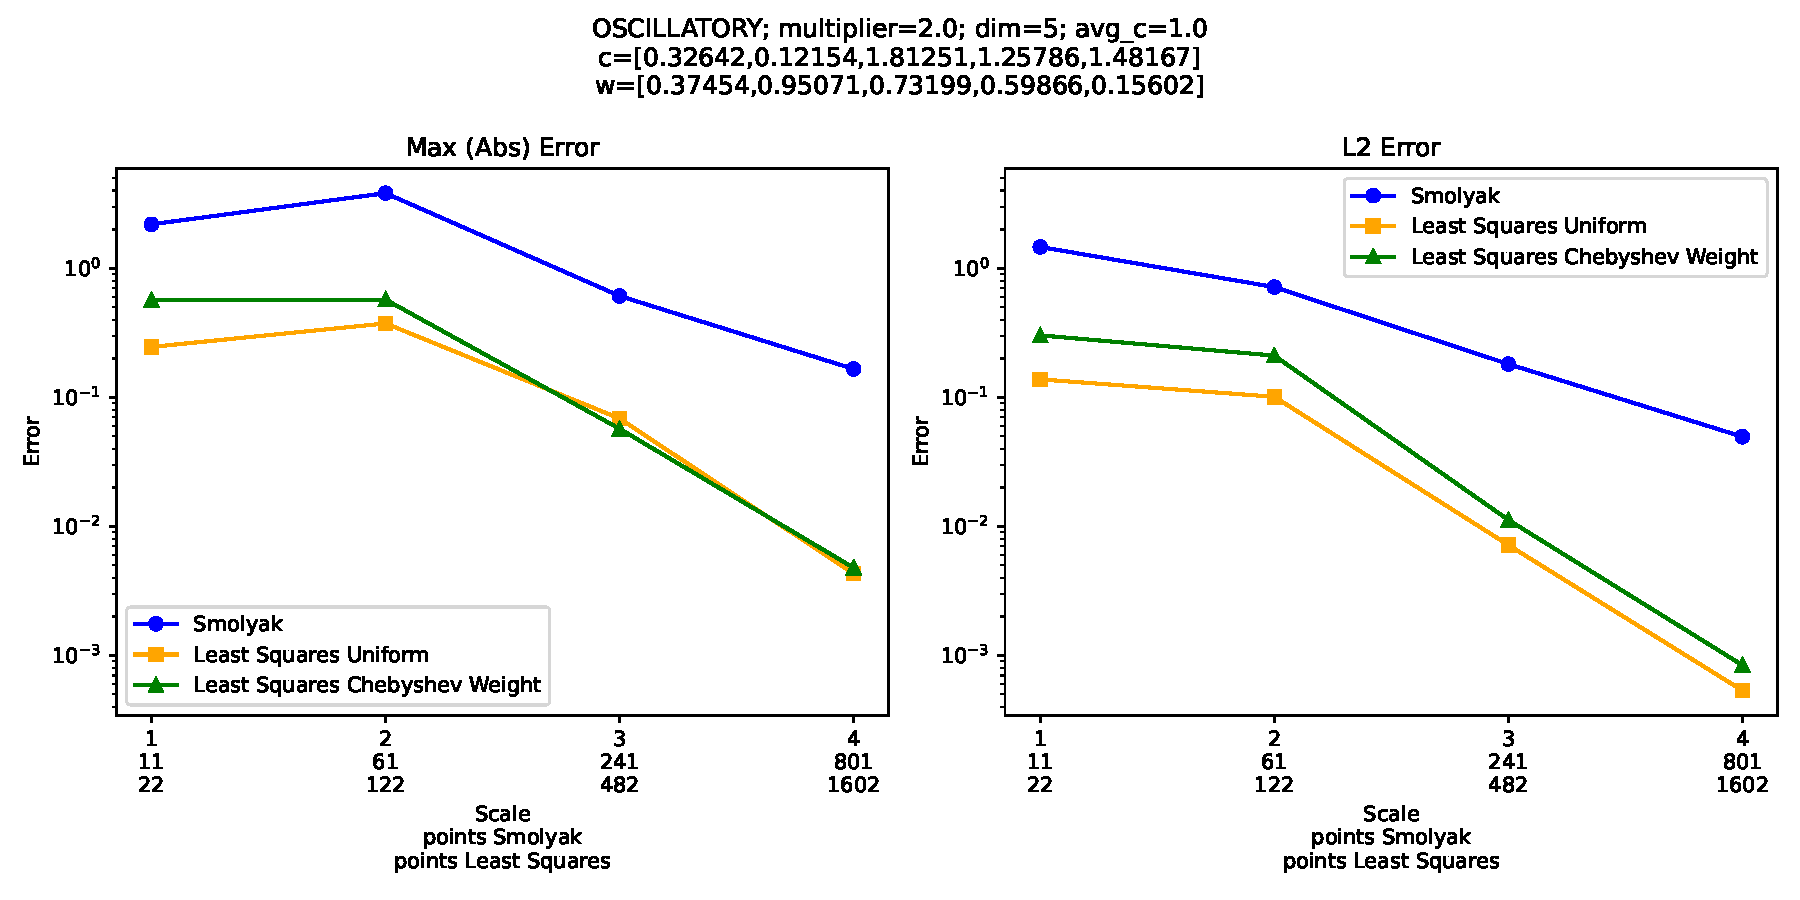
\includegraphics[width=\linewidth]{figures/oscillatory/realization1_dim5_scale4.pdf}
%	\caption{Caption}
%	\label{fig:Osc_1_dim5_scale4}
%\end{figure}
%
%\begin{figure}[H]
%	\centering
%	
%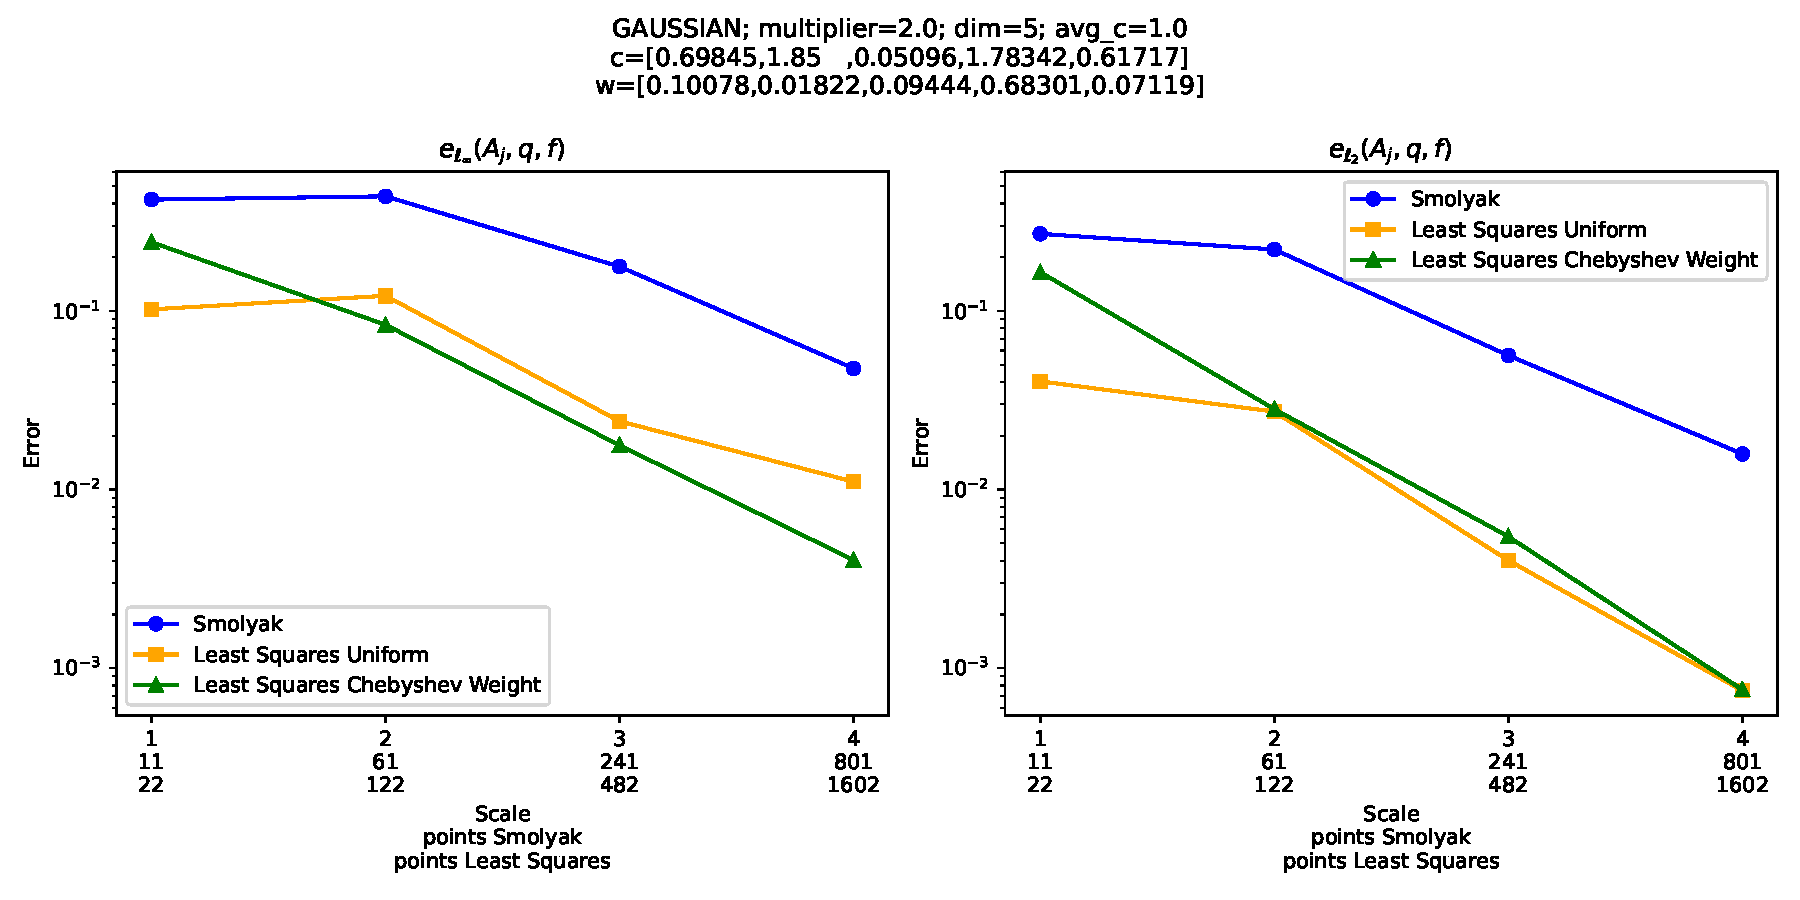
\includegraphics[width=\linewidth]{figures/oscillatory/realization2_dim5_scale4.pdf}
%	\caption{Caption}
%	\label{fig:Osc_2_dim5_scale4}
%\end{figure}
%
%\begin{figure}[H]
%	\centering
%	
%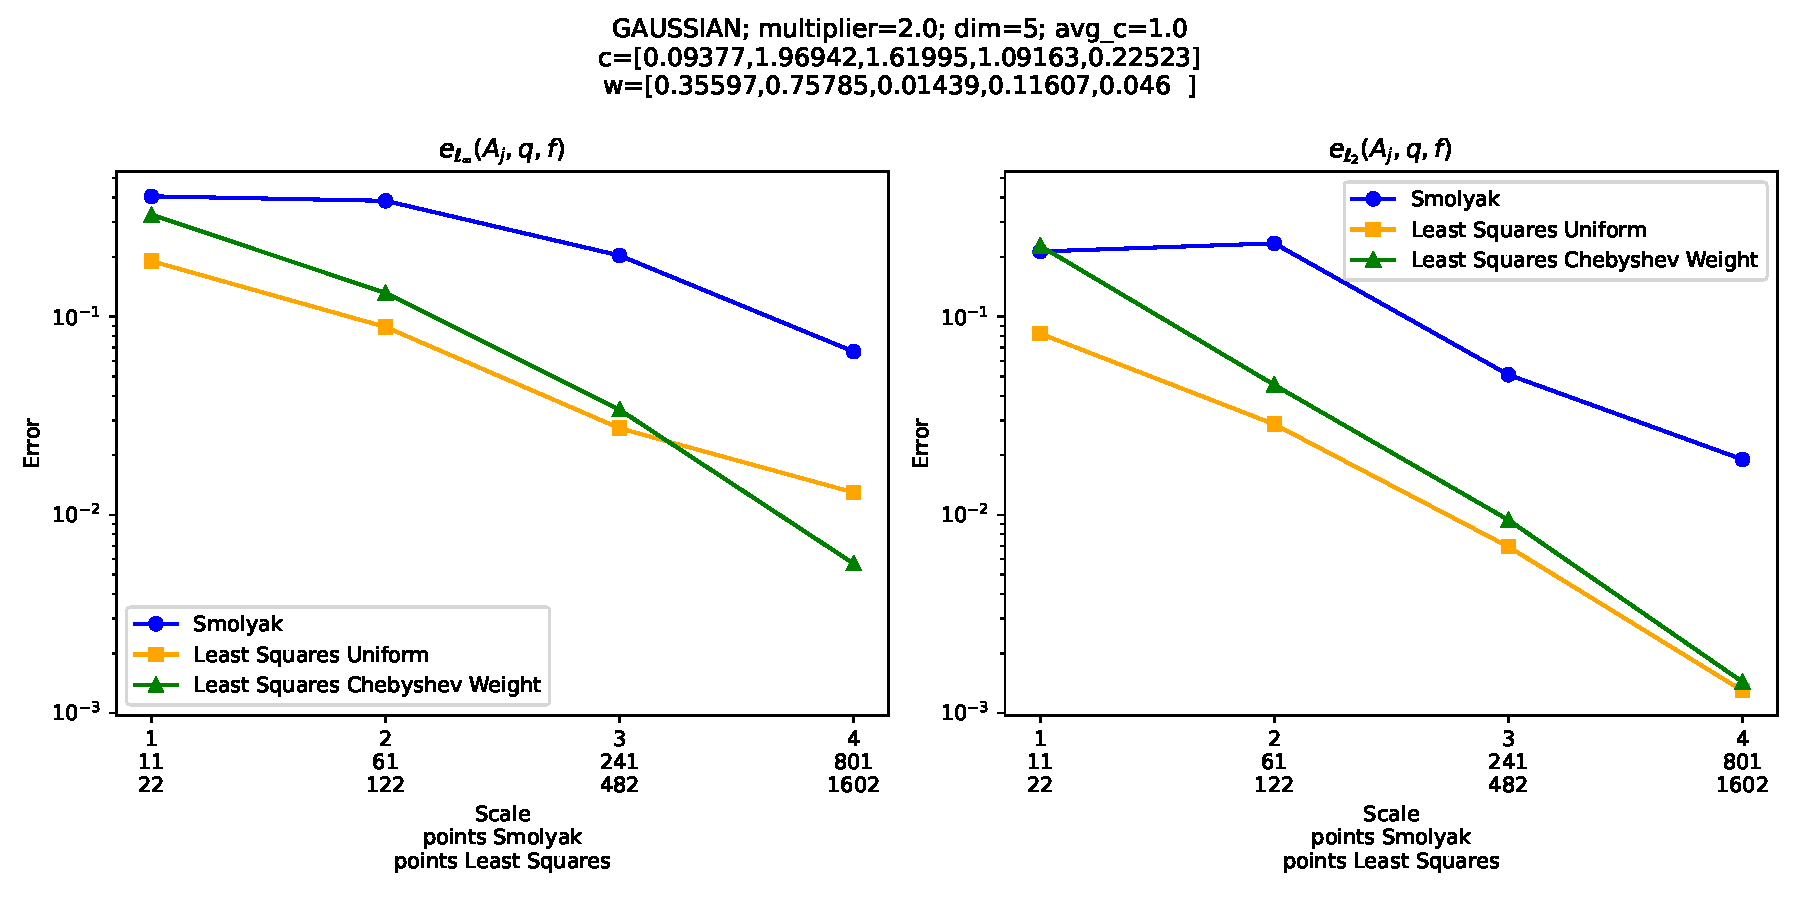
\includegraphics[width=\linewidth]{figures/oscillatory/realization3_dim5_scale4.pdf}
%	\caption{Caption}
%	\label{fig:Osc_3_dim5_scale4}
%\end{figure}
%
%\begin{figure}[H]
%	\centering
%	
%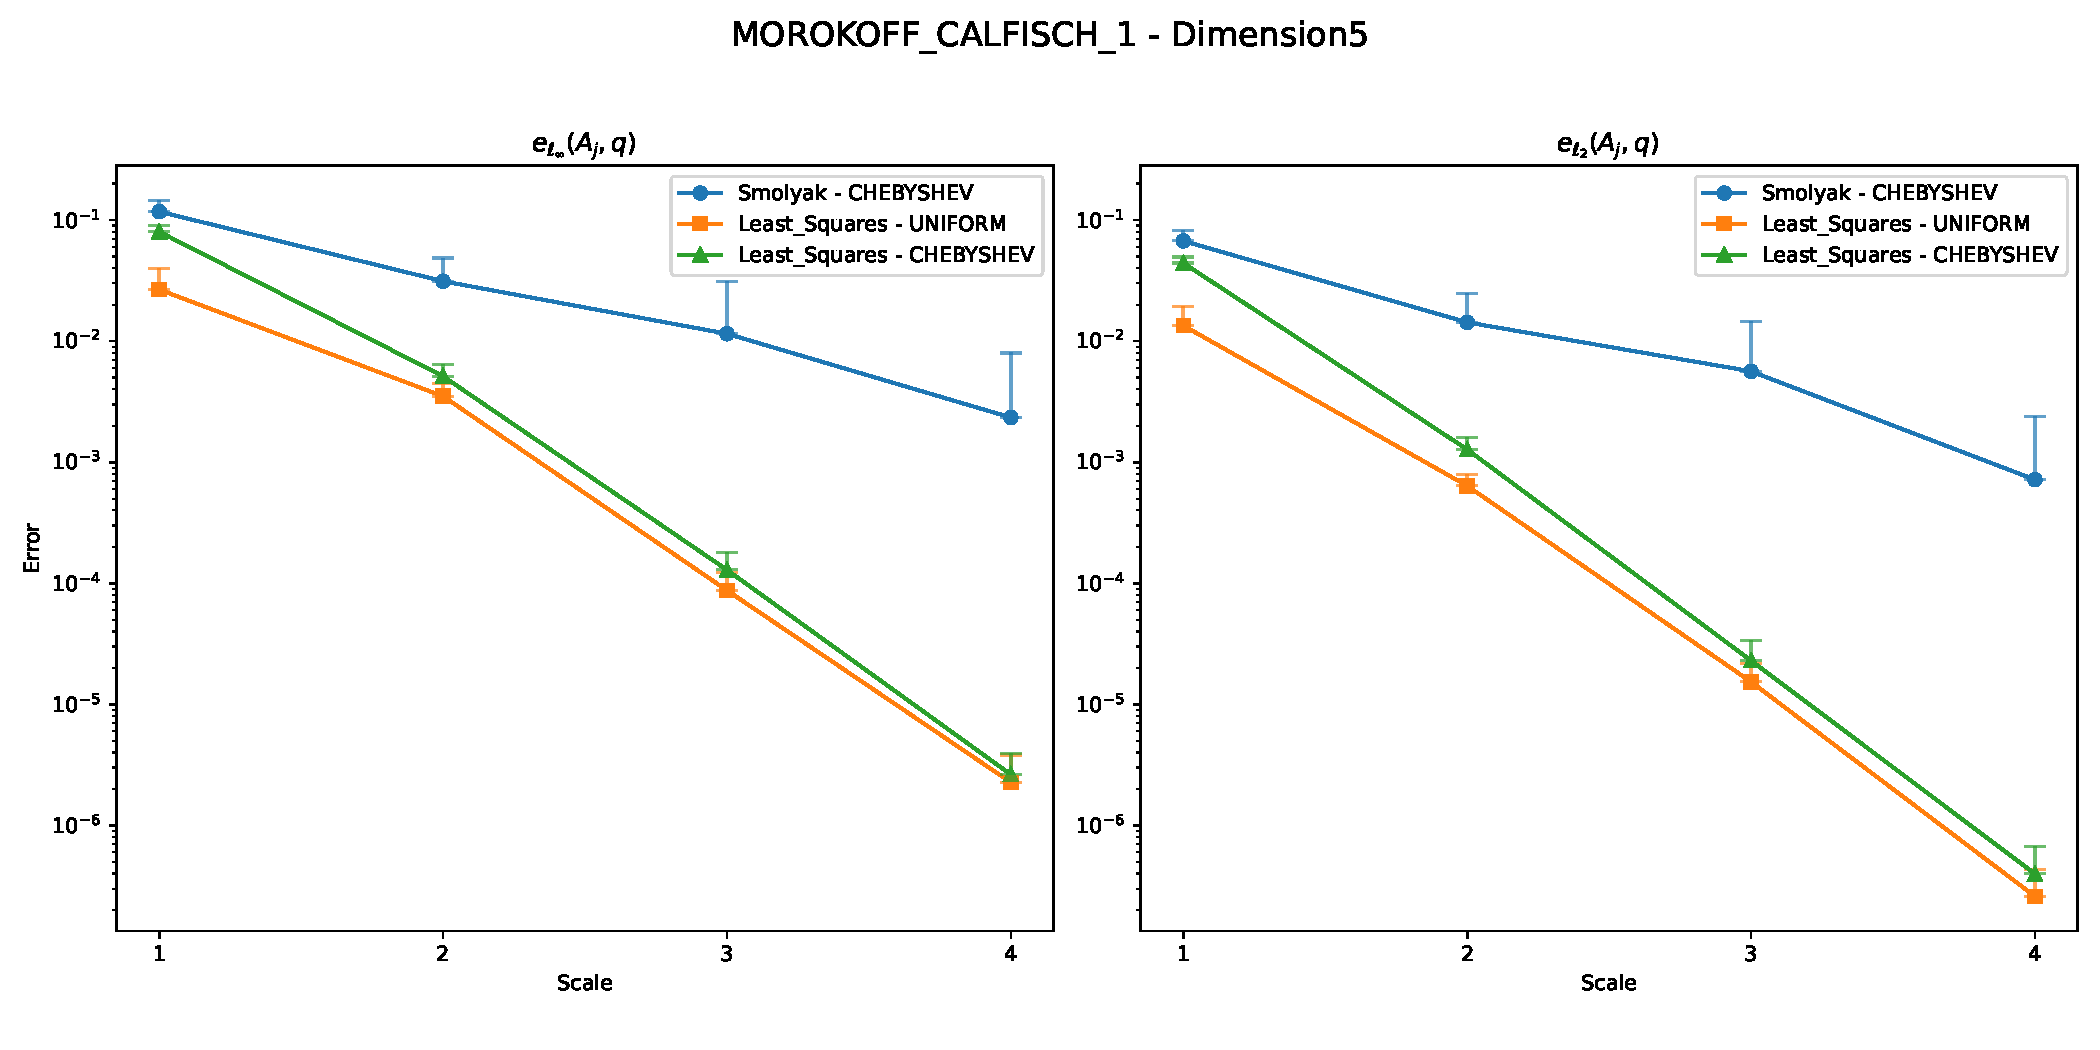
\includegraphics[width=\linewidth]{figures/morokoff_calfisch1/distro_dim5_scale4.pdf}
%	\caption{Caption}
%	\label{fig:morokoff_calfisch1_distribution_dim5_scale4}
%\end{figure}
%
%\begin{figure}[H]
%	\centering
%	
%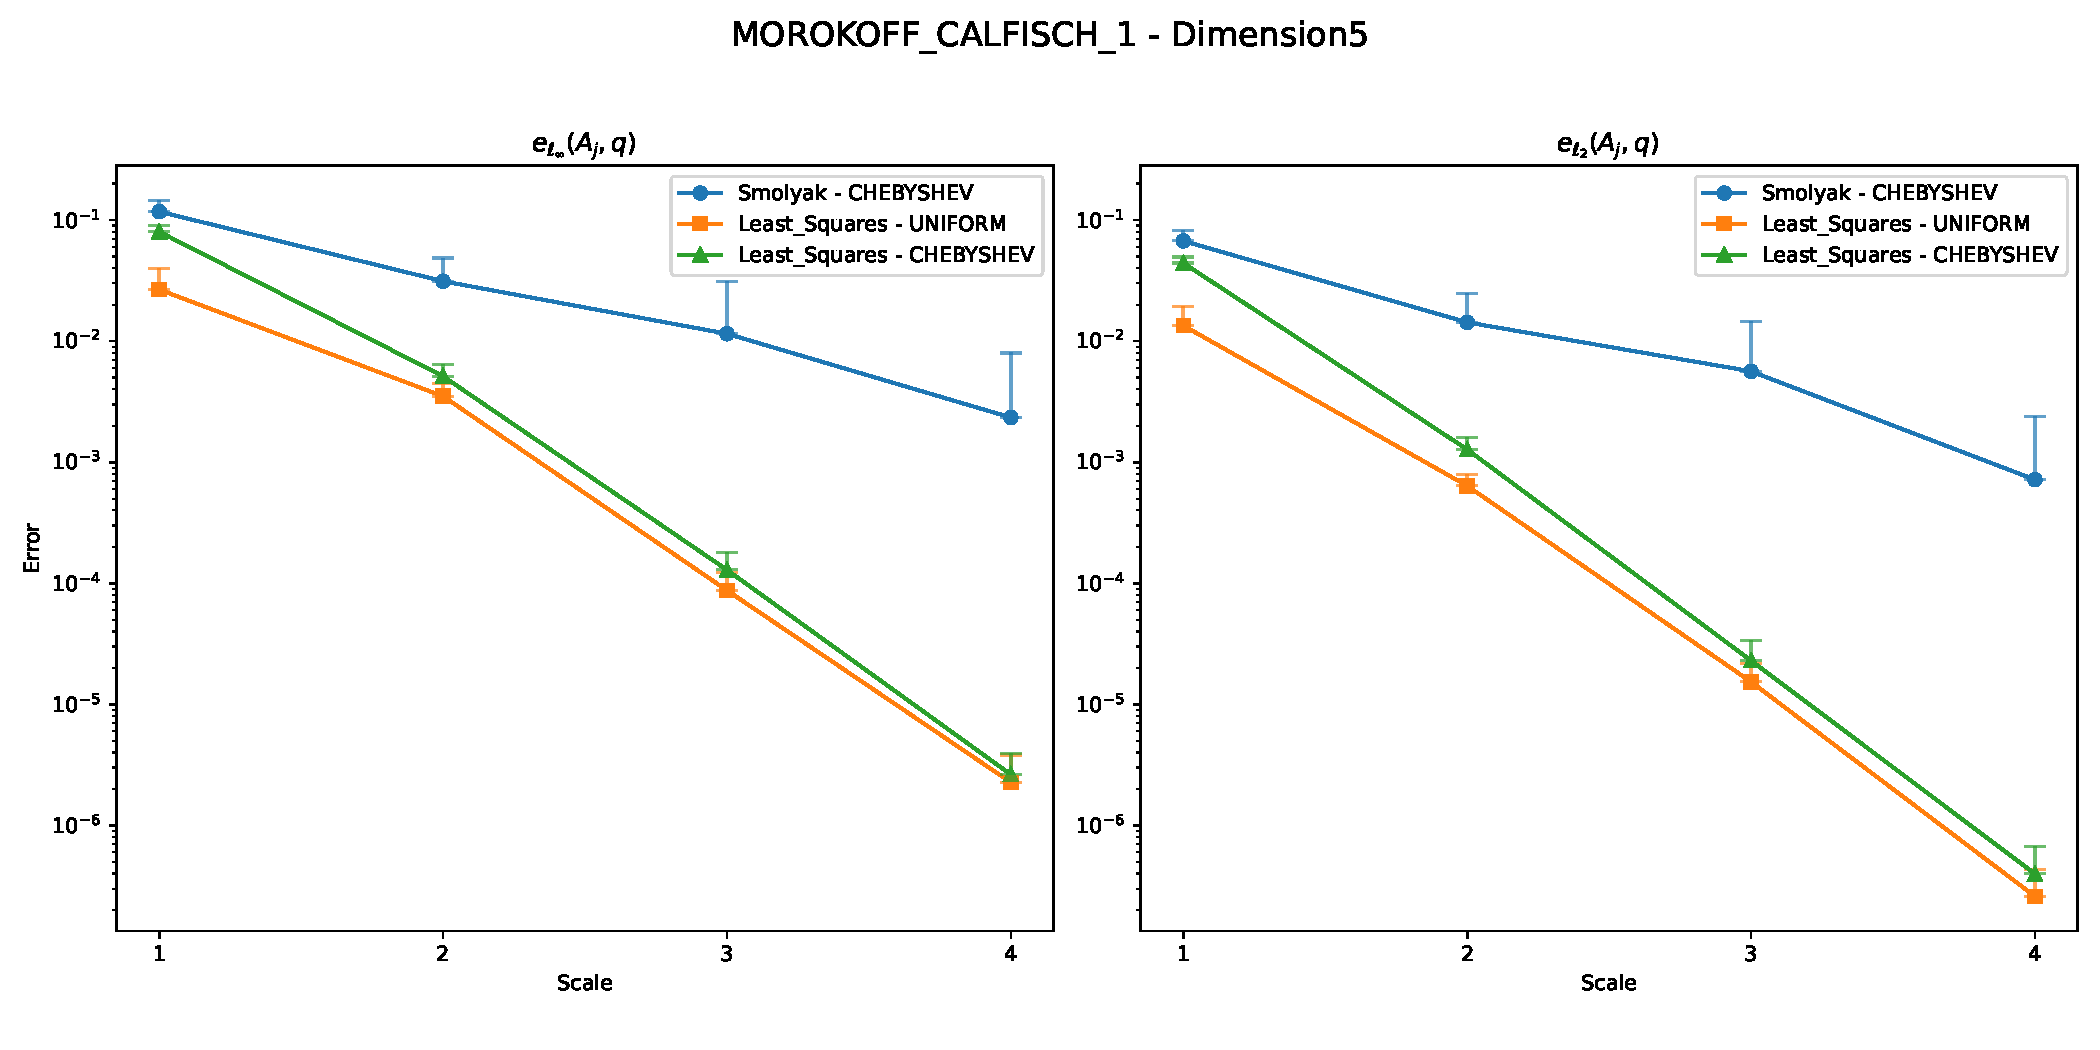
\includegraphics[width=\linewidth]{figures/morokoff_calfisch1/distro_dim5_scale4.pdf}
%	\caption{Caption}
%	\label{fig:morokoff_calfisch2_distribution_dim5_scale4}
%\end{figure}
%
%\begin{figure}[H] % TODO: Still with boxplot -> Maybe change
%	\centering
%	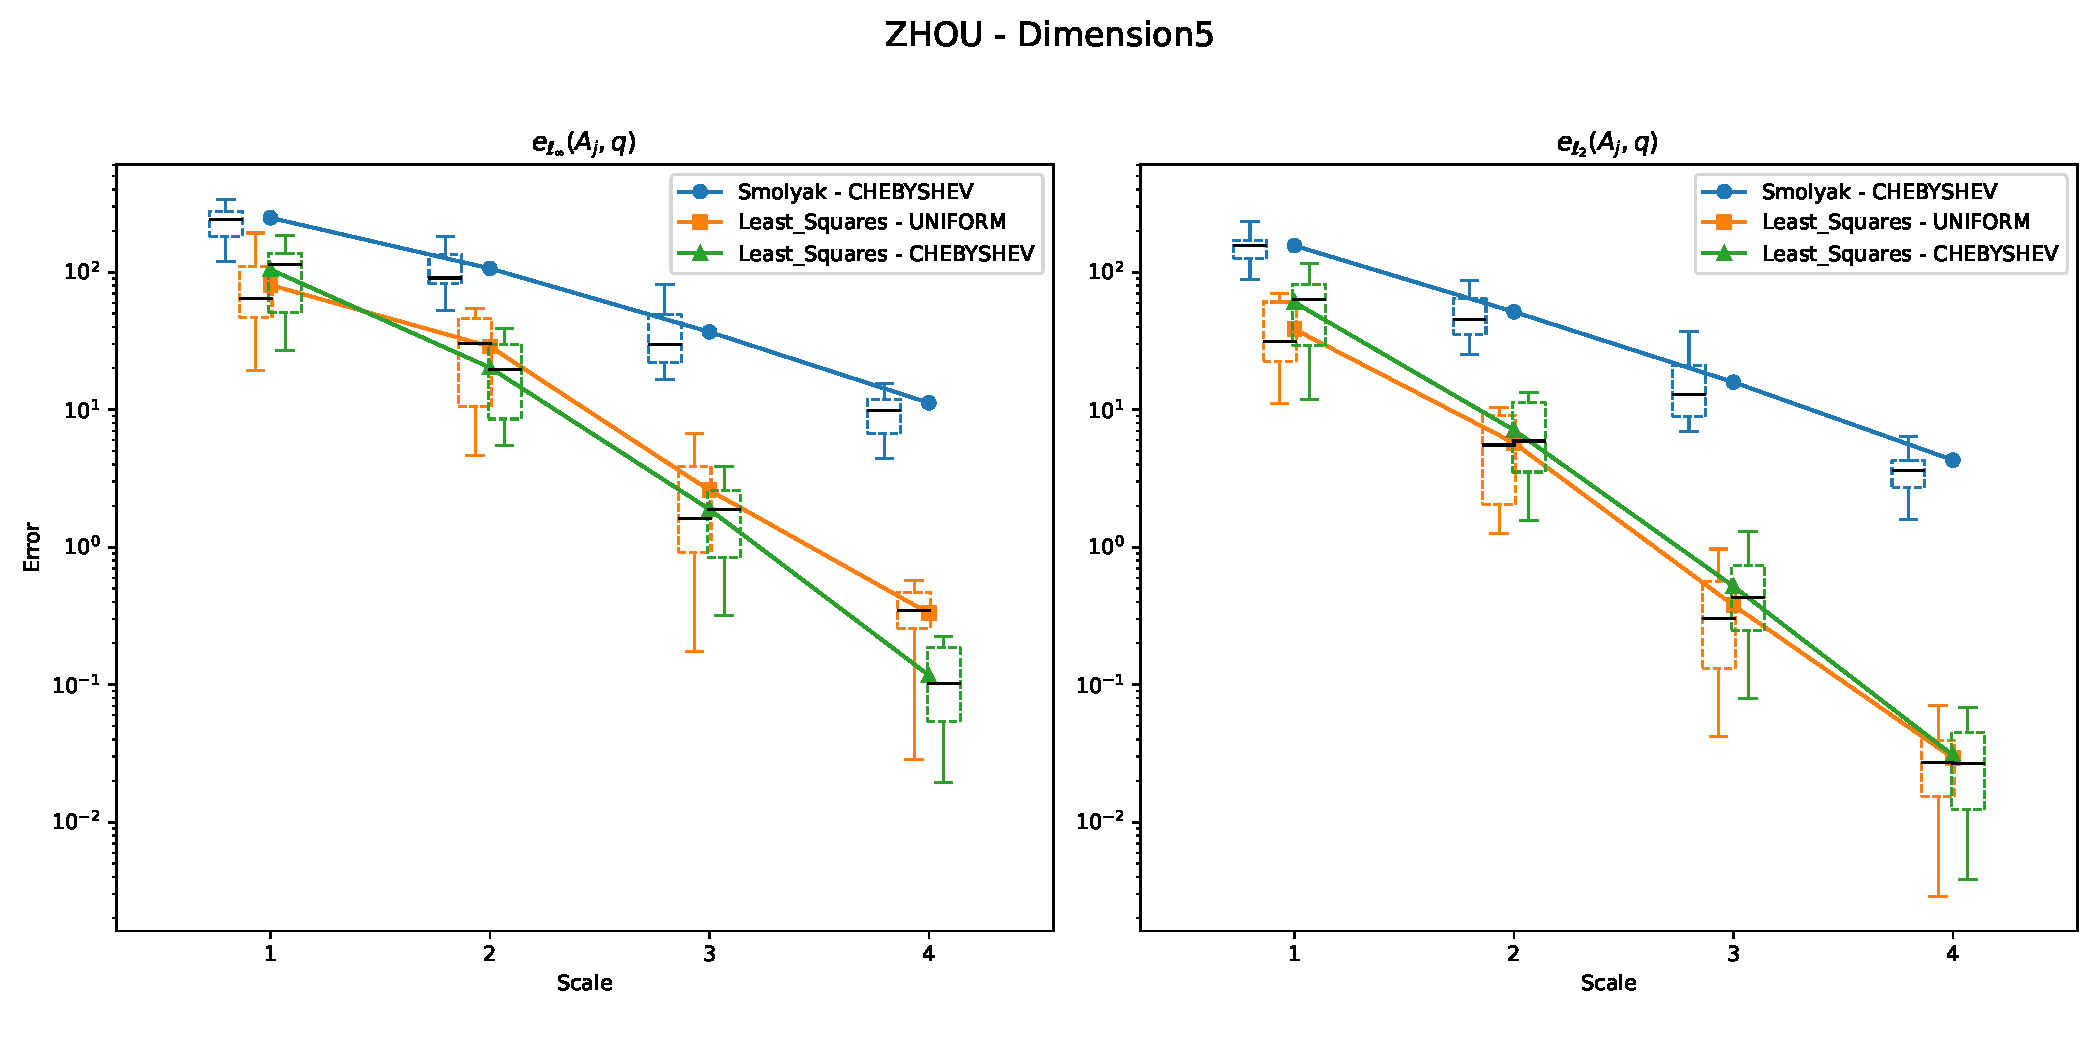
\includegraphics[width=\linewidth]{figures/zhou/distro_dim5_scale4.pdf}
%	\caption{Caption}
%	\label{fig:zhou_distribution_dim5_scale4}
%\end{figure}

\begin{table}[H]
	\centering
	\begin{adjustbox}{width=\linewidth}
		% Created with Python on 2025-06-15 11:13:45
% ..\results\final_results\low_dim\results_numerical_experiments.csv, dim=2, scales = [3, 4, 5, 6, 7, 8, 9]
\begin{tabular}{ll|rr|rr|rr|rr|rr|rr|rr|}
 &   \multicolumn{1}{c}{} & \multicolumn{2}{c}{Scale 3} & \multicolumn{2}{c}{Scale 4} & \multicolumn{2}{c}{Scale 5} & \multicolumn{2}{c}{Scale 6} & \multicolumn{2}{c}{Scale 7} & \multicolumn{2}{c}{Scale 8} & \multicolumn{2}{c}{Scale 9}\\
 &   \multicolumn{1}{c}{} & \multicolumn{1}{c}{$e_{\rm max}^{\rm wc}$} & \multicolumn{1}{c}{$e_{\rm mean}^{\rm wc}$} & \multicolumn{1}{c}{$e_{\rm max}^{\rm wc}$} & \multicolumn{1}{c}{$e_{\rm mean}^{\rm wc}$} & \multicolumn{1}{c}{$e_{\rm max}^{\rm wc}$} & \multicolumn{1}{c}{$e_{\rm mean}^{\rm wc}$} & \multicolumn{1}{c}{$e_{\rm max}^{\rm wc}$} & \multicolumn{1}{c}{$e_{\rm mean}^{\rm wc}$} & \multicolumn{1}{c}{$e_{\rm max}^{\rm wc}$} & \multicolumn{1}{c}{$e_{\rm mean}^{\rm wc}$} & \multicolumn{1}{c}{$e_{\rm max}^{\rm wc}$} & \multicolumn{1}{c}{$e_{\rm mean}^{\rm wc}$} & \multicolumn{1}{c}{$e_{\rm max}^{\rm wc}$} & \multicolumn{1}{c}{$e_{\rm mean}^{\rm wc}$}\\
\toprule
\multirow{3}{*}{\thead[l]{\tiny\textbf{Bim. Gauss.}\\$Q=50$}} & Smolyak & \first{5.71e-01} & \first{2.69e-01}  & \first{3.66e-01} & 1.55e-01  & 1.91e-01 & 7.14e-02  & 3.33e-02 & 9.39e-03  & 2.47e-03 & 6.16e-04  & 8.96e-06 & 2.44e-06  & 7.95e-09 & 2.19e-09\\
 & LS-Uniform & 3.51e+00 & 8.16e-01  & 5.12e+00 & 7.82e-01  & 3.56e+00 & 3.27e-01  & 8.19e+00 & 7.13e-01  & 3.15e+02 & 1.41e+01  & 1.93e+00 & 6.95e-02  & 3.03e+04 & 5.31e+02\\
 & LS-Chebyshev & 7.40e-01 & 2.89e-01  & 4.20e-01 & \first{1.35e-01}  & \first{1.87e-01} & \first{4.82e-02}  & \first{2.24e-02} & \first{6.11e-03}  & \first{1.52e-03} & \first{4.10e-04}  & \first{6.78e-06} & \first{1.50e-06}  & \first{7.27e-09} & \first{1.52e-09}\\
\midrule
\multirow{3}{*}{\thead[l]{\tiny\textbf{Cont.}\\$Q=50$}} & Smolyak & \first{4.40e-02} & \first{1.49e-02}  & 2.22e-02 & 5.15e-03  & 1.10e-02 & 1.58e-03  & 5.23e-03 & 6.18e-04  & 2.68e-03 & 2.17e-04  & 1.46e-03 & 8.93e-05  & 7.65e-04 & 2.95e-05\\
 & LS-Uniform & 2.66e-01 & 7.08e-02  & 5.19e-01 & 7.51e-02  & 3.64e-01 & 3.24e-02  & 6.88e-01 & 6.27e-02  & 5.86e+02 & 2.69e+01  & 7.77e+02 & 3.19e+01  & 8.46e+08 & 1.50e+07\\
 & LS-Chebyshev & 4.80e-02 & 2.21e-02  & \first{1.84e-02} & \first{4.06e-03}  & \first{9.43e-03} & \first{1.45e-03}  & \first{4.69e-03} & \first{4.91e-04}  & \first{2.08e-03} & \first{1.85e-04}  & \first{1.20e-03} & \first{6.72e-05}  & \first{6.47e-04} & \first{2.71e-05}\\
\midrule
\multirow{3}{*}{\thead[l]{\tiny\textbf{Corner Peak}\\$Q=50$}} & Smolyak & \first{8.78e-03} & 4.52e-03  & 1.48e-03 & 5.81e-04  & 1.04e-04 & 3.31e-05  & 8.90e-07 & 2.61e-07  & \first{6.08e-09} & 1.75e-09  & \first{2.77e-13} & 8.54e-14  & \first{6.99e-15} & \first{9.35e-16}\\
 & LS-Uniform & 1.54e-02 & 3.24e-03  & 3.50e-03 & 5.50e-04  & 4.92e-04 & 5.98e-05  & 2.30e-04 & 2.04e-05  & 6.80e-04 & 3.05e-05  & 7.93e-08 & 2.70e-09  & 1.66e-02 & 2.92e-04\\
 & LS-Chebyshev & 8.88e-03 & \first{3.12e-03}  & \first{1.42e-03} & \first{4.44e-04}  & \first{8.77e-05} & \first{2.65e-05}  & \first{6.13e-07} & \first{1.70e-07}  & 6.32e-09 & \first{1.30e-09}  & 2.79e-13 & \first{5.98e-14}  & 1.39e-14 & 1.17e-15\\
\midrule
\multirow{3}{*}{\thead[l]{\tiny\textbf{Discont.}\\$Q=50$}} & Smolyak & 4.73e+00 & \first{1.26e+00}  & 3.82e+00 & 1.08e+00  & 4.82e+00 & 8.42e-01  & 4.56e+00 & 6.75e-01  & 4.07e+00 & 4.26e-01  & 3.57e+00 & 3.28e-01  & 4.70e+00 & 2.16e-01\\
 & LS-Uniform & 3.46e+01 & 8.99e+00  & 7.48e+01 & 1.09e+01  & 6.02e+01 & 6.33e+00  & 3.07e+02 & 2.72e+01  & 6.62e+05 & 2.77e+04  & 1.79e+06 & 6.20e+04  & 6.27e+12 & 1.10e+11\\
 & LS-Chebyshev & \first{3.47e+00} & 1.27e+00  & \first{3.59e+00} & \first{7.15e-01}  & \first{4.24e+00} & \first{6.58e-01}  & \first{3.44e+00} & \first{4.35e-01}  & \first{3.25e+00} & \first{2.92e-01}  & \first{2.36e+00} & \first{2.04e-01}  & \first{2.92e+00} & \first{1.46e-01}\\
\midrule
\multirow{3}{*}{\thead[l]{\tiny\textbf{Gauss.}\\$Q=50$}} & Smolyak & 5.81e-01 & 2.39e-01  & 3.51e-01 & 9.72e-02  & 1.18e-01 & 3.11e-02  & 2.17e-02 & 5.03e-03  & 1.93e-03 & 4.27e-04  & 7.40e-06 & 1.88e-06  & 6.31e-09 & 1.51e-09\\
 & LS-Uniform & 3.13e+00 & 7.97e-01  & 3.83e+00 & 5.77e-01  & 3.44e+00 & 2.92e-01  & 7.53e+00 & 6.71e-01  & 2.27e+02 & 1.11e+01  & 2.62e+00 & 8.97e-02  & 1.88e+04 & 3.30e+02\\
 & LS-Chebyshev & \first{4.84e-01} & \first{1.75e-01}  & \first{3.40e-01} & \first{8.12e-02}  & \first{6.74e-02} & \first{1.90e-02}  & \first{1.67e-02} & \first{3.37e-03}  & \first{1.19e-03} & \first{2.87e-04}  & \first{5.39e-06} & \first{1.22e-06}  & \first{5.51e-09} & \first{1.08e-09}\\
\midrule
\multirow{3}{*}{\thead[l]{\tiny\textbf{Geo. Mean}\\$Q=50$}} & Smolyak & 1.09e-02 & 5.50e-03  & 2.80e-03 & \first{7.19e-04}  & \first{3.70e-04} & \first{7.25e-05}  & 4.84e-05 & 8.72e-06  & 3.65e-06 & 6.94e-07  & 1.36e-07 & 2.22e-08  & 2.19e-09 & 3.61e-10\\
 & LS-Uniform & \first{7.18e-03} & \first{1.52e-03}  & 5.70e-03 & 1.08e-03  & 1.33e-03 & 1.36e-04  & 3.29e-03 & 2.95e-04  & 1.07e-01 & 4.54e-03  & 3.88e-03 & 1.23e-04  & 2.26e+02 & 3.95e+00\\
 & LS-Chebyshev & 9.32e-03 & 4.52e-03  & \first{2.45e-03} & 9.90e-04  & 5.63e-04 & 9.85e-05  & \first{3.23e-05} & \first{7.11e-06}  & \first{3.08e-06} & \first{5.99e-07}  & \first{9.87e-08} & \first{2.00e-08}  & \first{2.06e-09} & \first{3.03e-10}\\
\midrule
\multirow{3}{*}{\thead[l]{\tiny\textbf{NOISE}\\$Q=50$}} & Smolyak & 6.00e-07 & 3.07e-07  & 6.46e-07 & 2.64e-07  & 7.78e-07 & 2.43e-07  & \first{8.85e-07} & 2.38e-07  & 9.21e-07 & 2.39e-07  & 1.21e-06 & 2.51e-07  & 1.25e-06 & 2.57e-07\\
 & LS-Uniform & 4.11e-06 & 1.04e-06  & 2.12e-05 & 3.07e-06  & 1.98e-05 & 2.30e-06  & 2.21e-04 & 2.00e-05  & 5.97e-01 & 2.69e-02  & 1.65e+00 & 5.52e-02  & 1.05e+07 & 1.84e+05\\
 & LS-Chebyshev & \first{5.59e-07} & \first{2.36e-07}  & \first{5.80e-07} & \first{1.97e-07}  & \first{7.30e-07} & \first{1.51e-07}  & 1.13e-06 & \first{1.47e-07}  & \first{8.96e-07} & \first{1.35e-07}  & \first{7.56e-07} & \first{1.28e-07}  & \first{7.61e-07} & \first{1.27e-07}\\
\midrule
\multirow{3}{*}{\thead[l]{\tiny\textbf{Osci.}\\$Q=50$}} & Smolyak & \first{3.97e-02} & 2.52e-02  & \first{2.12e-03} & 1.06e-03  & \first{4.48e-05} & 1.87e-05  & 9.42e-09 & 3.35e-09  & 5.70e-13 & 1.95e-13  & \first{9.44e-15} & \first{2.26e-15}  & \first{1.97e-14} & 3.65e-15\\
 & LS-Uniform & 1.69e-01 & 3.71e-02  & 9.31e-03 & 1.42e-03  & 1.97e-04 & 3.00e-05  & 2.71e-06 & 2.40e-07  & 7.01e-08 & 3.60e-09  & 7.54e-09 & 2.53e-10  & 5.83e-02 & 1.02e-03\\
 & LS-Chebyshev & 4.57e-02 & \first{1.78e-02}  & 2.53e-03 & \first{8.35e-04}  & 5.56e-05 & \first{1.33e-05}  & \first{7.69e-09} & \first{2.20e-09}  & \first{5.26e-13} & \first{1.40e-13}  & 3.43e-14 & 2.88e-15  & 2.81e-14 & \first{2.41e-15}\\
\midrule
\multirow{3}{*}{\thead[l]{\tiny\textbf{Prod. Peak}\\$Q=50$}} & Smolyak & \first{1.04e-03} & 6.17e-04  & \first{8.63e-05} & 3.77e-05  & 3.51e-06 & 1.24e-06  & 2.27e-08 & 7.41e-09  & 3.03e-11 & 8.55e-12  & \first{7.77e-15} & 2.15e-15  & \first{1.80e-14} & 3.63e-15\\
 & LS-Uniform & 4.27e-03 & 9.86e-04  & 4.65e-04 & 7.06e-05  & 1.99e-05 & 2.55e-06  & 7.28e-06 & 6.43e-07  & 3.65e-06 & 1.54e-07  & 3.19e-09 & 1.14e-10  & 2.16e-02 & 3.83e-04\\
 & LS-Chebyshev & 1.05e-03 & \first{5.03e-04}  & 1.01e-04 & \first{3.20e-05}  & \first{3.45e-06} & \first{8.70e-07}  & \first{1.81e-08} & \first{4.66e-09}  & \first{2.75e-11} & \first{6.14e-12}  & 1.55e-14 & \first{1.79e-15}  & 2.56e-14 & \first{1.73e-15}\\
\midrule
\multirow{3}{*}{\thead[l]{\tiny\textbf{Ridge Prod.}\\$Q=50$}} & Smolyak & 2.48e-01 & 1.05e-01  & \first{1.14e-01} & \first{3.85e-02}  & \first{6.89e-02} & 1.54e-02  & \first{3.42e-02} & 5.39e-03  & \first{2.39e-02} & 2.13e-03  & 1.18e-02 & 9.11e-04  & 7.14e-03 & 3.33e-04\\
 & LS-Uniform & 1.29e+00 & 3.18e-01  & 2.37e+00 & 3.45e-01  & 1.61e+00 & 1.67e-01  & 9.01e+00 & 7.85e-01  & 6.36e+03 & 2.86e+02  & 5.10e+03 & 1.54e+02  & 1.57e+10 & 2.75e+08\\
 & LS-Chebyshev & \first{1.94e-01} & \first{6.80e-02}  & 1.17e-01 & 4.08e-02  & 8.27e-02 & \first{1.14e-02}  & 4.75e-02 & \first{4.39e-03}  & 2.72e-02 & \first{1.68e-03}  & \first{1.14e-02} & \first{6.19e-04}  & \first{5.41e-03} & \first{2.38e-04}\\
\bottomrule
\end{tabular}

	\end{adjustbox}
	\caption{\StandardCaptionDimTable{2}{25}}
	\label{tab:dim2_results}
\end{table}

\begin{table}[H]
	\centering
	\begin{adjustbox}{width=\linewidth}
		% Created with Python on 2025-06-22 19:31:16
% ..\results\final_results\low_dim\results_numerical_experiments.csv, dim=3, scales = [3, 4, 5, 6, 7, 8, 9]
\begin{tabular}{ll|rr|rr|rr|rr|rr|rr|rr|}
 &   \multicolumn{1}{c}{} & \multicolumn{2}{c}{Scale 3} & \multicolumn{2}{c}{Scale 4} & \multicolumn{2}{c}{Scale 5} & \multicolumn{2}{c}{Scale 6} & \multicolumn{2}{c}{Scale 7} & \multicolumn{2}{c}{Scale 8} & \multicolumn{2}{c}{Scale 9}\\
 &   \multicolumn{1}{c}{} & \multicolumn{1}{c}{$e_{\rm max}^{\rm wc}$} & \multicolumn{1}{c}{$e_{\rm mean}^{\rm wc}$} & \multicolumn{1}{c}{$e_{\rm max}^{\rm wc}$} & \multicolumn{1}{c}{$e_{\rm mean}^{\rm wc}$} & \multicolumn{1}{c}{$e_{\rm max}^{\rm wc}$} & \multicolumn{1}{c}{$e_{\rm mean}^{\rm wc}$} & \multicolumn{1}{c}{$e_{\rm max}^{\rm wc}$} & \multicolumn{1}{c}{$e_{\rm mean}^{\rm wc}$} & \multicolumn{1}{c}{$e_{\rm max}^{\rm wc}$} & \multicolumn{1}{c}{$e_{\rm mean}^{\rm wc}$} & \multicolumn{1}{c}{$e_{\rm max}^{\rm wc}$} & \multicolumn{1}{c}{$e_{\rm mean}^{\rm wc}$} & \multicolumn{1}{c}{$e_{\rm max}^{\rm wc}$} & \multicolumn{1}{c}{$e_{\rm mean}^{\rm wc}$}\\
\toprule
\multirow{3}{*}{\thead[l]{\tiny\textbf{Bim. Gauss.}\\$Q=50$}} & Smolyak & 7.17e-01 & 2.93e-01  & \first{4.04e-01} & 1.43e-01  & 2.98e-01 & 8.74e-02  & 1.06e-01 & 2.28e-02  & 2.71e-02 & 5.99e-03  & 5.82e-03 & 9.34e-04  & 6.64e-04 & 1.12e-04\\
 & LS-Uniform & 2.47e+00 & 4.44e-01  & 1.33e+00 & 2.13e-01  & 8.83e-01 & 1.27e-01  & 1.37e+00 & 6.60e-02  & 7.62e-01 & 2.36e-02  & 1.42e+00 & 2.36e-02  & 4.05e+01 & 4.14e-01\\
 & LS-Chebyshev & \first{6.04e-01} & \first{1.77e-01}  & 5.85e-01 & \first{1.25e-01}  & \first{2.25e-01} & \first{5.65e-02}  & \first{7.17e-02} & \first{1.27e-02}  & \first{2.26e-02} & \first{2.86e-03}  & \first{3.83e-03} & \first{4.99e-04}  & \first{3.65e-04} & \first{5.14e-05}\\
\midrule
\multirow{3}{*}{\thead[l]{\tiny\textbf{Cont.}\\$Q=50$}} & Smolyak & 4.54e-02 & 1.16e-02  & \first{1.57e-02} & \first{3.66e-03}  & 1.17e-02 & 1.68e-03  & \first{4.17e-03} & \first{4.94e-04}  & 3.22e-03 & 1.92e-04  & 1.32e-03 & 6.54e-05  & 6.66e-04 & 2.43e-05\\
 & LS-Uniform & 9.00e-02 & 1.51e-02  & 2.57e-02 & 4.94e-03  & 3.90e-02 & 2.89e-03  & 5.98e-02 & 2.11e-03  & 5.33e-02 & 1.49e-03  & 2.74e-01 & 4.00e-03  & 3.04e+01 & 3.14e-01\\
 & LS-Chebyshev & \first{3.30e-02} & \first{9.08e-03}  & 1.90e-02 & 4.16e-03  & \first{7.98e-03} & \first{1.43e-03}  & 5.42e-03 & 5.28e-04  & \first{2.11e-03} & \first{1.81e-04}  & \first{1.04e-03} & \first{6.09e-05}  & \first{5.69e-04} & \first{2.19e-05}\\
\midrule
\multirow{3}{*}{\thead[l]{\tiny\textbf{Corner Peak}\\$Q=50$}} & Smolyak & 5.78e-02 & 1.58e-02  & 3.03e-02 & 5.80e-03  & 7.48e-03 & 1.46e-03  & 1.44e-03 & 2.55e-04  & 1.98e-04 & 2.96e-05  & 1.35e-05 & 2.06e-06  & 3.16e-07 & 4.17e-08\\
 & LS-Uniform & 7.11e-02 & \first{1.33e-02}  & \first{8.54e-03} & \first{1.65e-03}  & 6.77e-03 & \first{3.90e-04}  & 2.03e-03 & 1.02e-04  & 1.40e-03 & 3.23e-05  & 6.45e-04 & 1.13e-05  & 5.31e-03 & 5.72e-05\\
 & LS-Chebyshev & \first{3.38e-02} & 1.34e-02  & 9.19e-03 & 2.33e-03  & \first{2.31e-03} & 4.72e-04  & \first{3.68e-04} & \first{8.59e-05}  & \first{6.43e-05} & \first{1.07e-05}  & \first{5.24e-06} & \first{9.96e-07}  & \first{1.16e-07} & \first{2.05e-08}\\
\midrule
\multirow{3}{*}{\thead[l]{\tiny\textbf{Discont.}\\$Q=50$}} & Smolyak & 7.08e+00 & \first{1.73e+00}  & 1.11e+01 & \first{1.33e+00}  & 7.35e+00 & \first{1.03e+00}  & 9.26e+00 & 8.10e-01  & 9.99e+00 & 5.76e-01  & 8.40e+00 & 4.81e-01  & 1.07e+01 & 3.28e-01\\
 & LS-Uniform & 1.70e+01 & 3.87e+00  & 1.11e+01 & 1.66e+00  & 2.38e+01 & 1.67e+00  & 6.09e+01 & 2.57e+00  & 2.28e+02 & 5.88e+00  & 1.29e+03 & 2.70e+01  & 4.47e+05 & 4.45e+03\\
 & LS-Chebyshev & \first{6.97e+00} & 1.75e+00  & \first{6.09e+00} & 1.37e+00  & \first{5.86e+00} & 1.04e+00  & \first{7.10e+00} & \first{7.63e-01}  & \first{9.30e+00} & \first{5.30e-01}  & \first{6.44e+00} & \first{3.77e-01}  & \first{6.29e+00} & \first{2.59e-01}\\
\midrule
\multirow{3}{*}{\thead[l]{\tiny\textbf{Gauss.}\\$Q=50$}} & Smolyak & 6.32e-01 & 2.17e-01  & 4.54e-01 & 9.92e-02  & \first{2.21e-01} & 3.99e-02  & 1.20e-01 & 1.72e-02  & 3.31e-02 & 5.10e-03  & 7.56e-03 & 8.69e-04  & 9.87e-04 & 1.01e-04\\
 & LS-Uniform & 1.66e+00 & 2.82e-01  & 7.59e-01 & 9.70e-02  & 7.69e-01 & 6.15e-02  & 6.03e-01 & 3.04e-02  & 6.14e-01 & 1.82e-02  & 9.04e-01 & 1.65e-02  & 5.56e+01 & 5.23e-01\\
 & LS-Chebyshev & \first{4.91e-01} & \first{1.28e-01}  & \first{3.66e-01} & \first{7.08e-02}  & 2.59e-01 & \first{2.74e-02}  & \first{9.23e-02} & \first{8.81e-03}  & \first{1.72e-02} & \first{2.09e-03}  & \first{2.88e-03} & \first{3.73e-04}  & \first{3.26e-04} & \first{4.46e-05}\\
\midrule
\multirow{3}{*}{\thead[l]{\tiny\textbf{Geo. Mean}\\$Q=50$}} & Smolyak & 2.27e-02 & 7.18e-03  & \first{3.20e-03} & 8.34e-04  & 3.76e-04 & 6.70e-05  & 2.58e-05 & 4.08e-06  & 2.11e-06 & 2.89e-07  & 1.44e-07 & 1.55e-08  & 6.94e-09 & 7.03e-10\\
 & LS-Uniform & 4.56e-02 & \first{6.02e-03}  & 4.19e-03 & \first{5.11e-04}  & 5.38e-04 & \first{4.27e-05}  & 5.83e-05 & 3.24e-06  & 3.39e-05 & 9.23e-07  & 1.81e-06 & 4.77e-08  & 6.44e-05 & 6.38e-07\\
 & LS-Chebyshev & \first{2.22e-02} & 6.15e-03  & 3.75e-03 & 1.06e-03  & \first{2.48e-04} & 7.25e-05  & \first{1.39e-05} & \first{3.05e-06}  & \first{9.97e-07} & \first{1.49e-07}  & \first{4.43e-08} & \first{6.60e-09}  & \first{2.38e-09} & \first{3.29e-10}\\
\midrule
\multirow{3}{*}{\thead[l]{\tiny\textbf{NOISE}\\$Q=50$}} & Smolyak & 9.86e-07 & 3.43e-07  & 1.25e-06 & 3.48e-07  & 1.44e-06 & 4.06e-07  & 1.80e-06 & 4.04e-07  & 2.24e-06 & 4.56e-07  & 2.73e-06 & 4.96e-07  & 3.06e-06 & 5.57e-07\\
 & LS-Uniform & 1.75e-06 & 3.59e-07  & 1.39e-06 & 2.47e-07  & 3.84e-06 & 3.29e-07  & 2.20e-05 & 8.19e-07  & 6.91e-05 & 1.80e-06  & 6.26e-04 & 1.09e-05  & 2.51e-01 & 2.57e-03\\
 & LS-Chebyshev & \first{6.16e-07} & \first{1.70e-07}  & \first{6.21e-07} & \first{1.59e-07}  & \first{6.35e-07} & \first{1.49e-07}  & \first{8.77e-07} & \first{1.46e-07}  & \first{9.05e-07} & \first{1.43e-07}  & \first{7.14e-07} & \first{1.38e-07}  & \first{7.36e-07} & \first{1.31e-07}\\
\midrule
\multirow{3}{*}{\thead[l]{\tiny\textbf{Osci.}\\$Q=50$}} & Smolyak & \first{4.60e-01} & \first{1.54e-01}  & \first{8.77e-02} & 3.12e-02  & 9.48e-03 & 3.25e-03  & 5.94e-04 & 1.77e-04  & 2.01e-05 & 4.99e-06  & 2.82e-07 & 6.29e-08  & 7.89e-11 & 1.71e-11\\
 & LS-Uniform & 1.12e+00 & 2.40e-01  & 1.43e-01 & \first{1.71e-02}  & 2.46e-02 & 1.93e-03  & 2.61e-03 & 1.24e-04  & 2.75e-04 & 7.39e-06  & 4.31e-05 & 7.63e-07  & 4.07e-06 & 3.67e-08\\
 & LS-Chebyshev & 6.95e-01 & 1.94e-01  & 9.86e-02 & 2.25e-02  & \first{8.00e-03} & \first{1.65e-03}  & \first{3.41e-04} & \first{7.41e-05}  & \first{1.38e-05} & \first{2.08e-06}  & \first{1.45e-07} & \first{2.87e-08}  & \first{4.98e-11} & \first{7.59e-12}\\
\midrule
\multirow{3}{*}{\thead[l]{\tiny\textbf{Prod. Peak}\\$Q=50$}} & Smolyak & 3.13e-03 & 1.28e-03  & 4.30e-04 & 1.57e-04  & 4.39e-05 & 1.56e-05  & 3.80e-06 & 1.11e-06  & 2.04e-07 & 4.59e-08  & 5.45e-09 & 9.51e-10  & 4.20e-11 & 7.27e-12\\
 & LS-Uniform & 9.12e-03 & 1.56e-03  & 5.74e-04 & \first{7.52e-05}  & 8.01e-05 & \first{8.11e-06}  & 1.44e-05 & 7.00e-07  & 2.28e-06 & 6.98e-08  & 9.92e-07 & 1.61e-08  & 1.46e-06 & 1.47e-08\\
 & LS-Chebyshev & \first{2.53e-03} & \first{1.04e-03}  & \first{4.28e-04} & 1.07e-04  & \first{3.82e-05} & 8.14e-06  & \first{2.77e-06} & \first{5.03e-07}  & \first{1.50e-07} & \first{2.05e-08}  & \first{2.57e-09} & \first{4.36e-10}  & \first{2.47e-11} & \first{3.23e-12}\\
\midrule
\multirow{3}{*}{\thead[l]{\tiny\textbf{Ridge Prod.}\\$Q=50$}} & Smolyak & 6.03e-01 & 1.98e-01  & 4.75e-01 & 8.99e-02  & 2.08e-01 & 4.03e-02  & 1.18e-01 & 1.54e-02  & 7.33e-02 & 6.44e-03  & \first{3.25e-02} & 2.47e-03  & 3.06e-02 & 9.64e-04\\
 & LS-Uniform & 1.09e+00 & 2.25e-01  & 4.55e-01 & 9.45e-02  & 4.46e-01 & 4.71e-02  & 9.80e-01 & 3.95e-02  & 2.31e+00 & 5.32e-02  & 1.25e+01 & 2.04e-01  & 2.03e+03 & 1.87e+01\\
 & LS-Chebyshev & \first{5.43e-01} & \first{1.53e-01}  & \first{3.43e-01} & \first{7.47e-02}  & \first{1.98e-01} & \first{3.08e-02}  & \first{9.31e-02} & \first{1.15e-02}  & \first{4.65e-02} & \first{4.66e-03}  & 3.39e-02 & \first{1.74e-03}  & \first{1.99e-02} & \first{6.82e-04}\\
\bottomrule
\end{tabular}

	\end{adjustbox}
	\caption{Dim 3}
	\label{tab:dim3_results}
\end{table}

\begin{table}[H]
	\centering
	\begin{adjustbox}{width=\linewidth}
		% Created with Python on 2025-05-29 10:15:57
% ..\results\final_results\results_numerical_experiments.csv, dim=4, scales = [3, 4, 5, 6, 7, 8, 9]
\begin{tabular}{ll|rr|rr|rr|rr|rr|rr|rr|}
 &   \multicolumn{1}{c}{} & \multicolumn{2}{c}{Scale3} & \multicolumn{2}{c}{Scale4} & \multicolumn{2}{c}{Scale5} & \multicolumn{2}{c}{Scale6} & \multicolumn{2}{c}{Scale7} & \multicolumn{2}{c}{Scale8} & \multicolumn{2}{c}{Scale9}\\
 &   \multicolumn{1}{c}{} & \multicolumn{1}{c}{$e_{\rm max}^{\rm wc}$} & \multicolumn{1}{c}{$e_{\rm mean}^{\rm wc}$} & \multicolumn{1}{c}{$e_{\rm max}^{\rm wc}$} & \multicolumn{1}{c}{$e_{\rm mean}^{\rm wc}$} & \multicolumn{1}{c}{$e_{\rm max}^{\rm wc}$} & \multicolumn{1}{c}{$e_{\rm mean}^{\rm wc}$} & \multicolumn{1}{c}{$e_{\rm max}^{\rm wc}$} & \multicolumn{1}{c}{$e_{\rm mean}^{\rm wc}$} & \multicolumn{1}{c}{$e_{\rm max}^{\rm wc}$} & \multicolumn{1}{c}{$e_{\rm mean}^{\rm wc}$} & \multicolumn{1}{c}{$e_{\rm max}^{\rm wc}$} & \multicolumn{1}{c}{$e_{\rm mean}^{\rm wc}$} & \multicolumn{1}{c}{$e_{\rm max}^{\rm wc}$} & \multicolumn{1}{c}{$e_{\rm mean}^{\rm wc}$}\\
\toprule
\multirow{3}{*}{\thead[l]{\tiny\textbf{Bim. Gauss.}\\$Q=10$}} & Smolyak & 8.98e-01 & 2.04e-01  & 8.55e-01 & 1.48e-01  & 5.99e-01 & 9.86e-02  & 4.13e-01 & 5.87e-02  & 2.78e-01 & 2.75e-02  & 1.87e-01 & 1.40e-02  & 8.42e-02 & 5.36e-03\\
 & LS-Uniform & 1.34e+00 & 2.27e-01  & 1.32e+00 & 1.25e-01  & 1.61e+00 & 1.14e-01  & 1.20e+00 & 5.98e-02  & 7.72e-01 & 3.02e-02  & 7.89e-01 & 1.46e-02  & 6.83e-01 & 7.05e-03\\
 & LS-Chebyshev & \first{5.76e-01} & \first{1.20e-01}  & \first{6.44e-01} & \first{9.35e-02}  & \first{4.86e-01} & \first{5.52e-02}  & \first{3.01e-01} & \first{2.84e-02}  & \first{1.75e-01} & \first{1.55e-02}  & \first{7.85e-02} & \first{6.31e-03}  & \first{3.84e-02} & \first{2.05e-03}\\
\midrule
\multirow{3}{*}{\thead[l]{\tiny\textbf{Cont.}\\$Q=25$}} & Smolyak & \first{1.16e-01} & 3.75e-02  & \first{5.44e-02} & 1.55e-02  & \first{3.96e-02} & 5.52e-03  & \first{2.29e-02} & 2.15e-03  & \first{1.42e-02} & 9.22e-04  & \first{1.04e-02} & 3.76e-04  & \first{4.97e-03} & 1.76e-04\\
 & LS-Uniform & 1.37e-01 & 2.70e-02  & 7.07e-02 & 1.09e-02  & 7.09e-02 & 6.80e-03  & 6.79e-02 & 2.87e-03  & 3.32e-02 & 1.55e-03  & 4.10e-02 & 8.18e-04  & 9.32e-02 & 6.25e-04\\
 & LS-Chebyshev & 1.19e-01 & \first{2.42e-02}  & 6.54e-02 & \first{9.02e-03}  & 4.28e-02 & \first{3.80e-03}  & 3.52e-02 & \first{1.79e-03}  & 1.95e-02 & \first{7.78e-04}  & 1.55e-02 & \first{3.32e-04}  & 9.79e-03 & \first{1.51e-04}\\
\midrule
\multirow{3}{*}{\thead[l]{\tiny\textbf{Corner Peak}\\$Q=25$}} & Smolyak & 1.64e-01 & 2.22e-02  & 8.03e-02 & 1.35e-02  & 5.32e-02 & 5.65e-03  & 1.81e-02 & 2.31e-03  & 6.36e-03 & 6.39e-04  & 1.55e-03 & 1.35e-04  & 3.04e-04 & 2.16e-05\\
 & LS-Uniform & \first{7.21e-02} & \first{9.98e-03}  & 4.68e-02 & \first{3.51e-03}  & 3.03e-02 & \first{1.34e-03}  & 1.08e-02 & \first{2.63e-04}  & 2.61e-03 & \first{5.53e-05}  & 1.35e-03 & \first{1.53e-05}  & 2.53e-04 & \first{2.87e-06}\\
 & LS-Chebyshev & 1.08e-01 & 3.67e-02  & \first{3.26e-02} & 8.27e-03  & \first{1.05e-02} & 2.20e-03  & \first{2.84e-03} & 5.13e-04  & \first{9.73e-04} & 1.41e-04  & \first{1.94e-04} & 2.97e-05  & \first{4.72e-05} & 5.95e-06\\
\midrule
\multirow{3}{*}{\thead[l]{\tiny\textbf{Discont.}\\$Q=25$}} & Smolyak & 2.15e+01 & 5.20e+00  & 2.32e+01 & 2.96e+00  & 2.51e+01 & 2.66e+00  & 1.88e+01 & 1.73e+00  & 2.16e+01 & 1.44e+00  & 2.74e+01 & 1.05e+00  & 2.60e+01 & \first{7.32e-01}\\
 & LS-Uniform & 2.31e+01 & 4.30e+00  & 3.05e+01 & \first{2.86e+00}  & 5.69e+01 & 3.68e+00  & 7.03e+01 & 3.26e+00  & 6.35e+01 & 2.47e+00  & 2.06e+02 & 2.95e+00  & 3.47e+02 & 3.06e+00\\
 & LS-Chebyshev & \first{1.27e+01} & \first{3.35e+00}  & \first{1.42e+01} & 3.79e+00  & \first{1.90e+01} & \first{2.37e+00}  & \first{1.65e+01} & \first{1.65e+00}  & \first{1.70e+01} & \first{1.44e+00}  & \first{1.88e+01} & \first{1.01e+00}  & \first{1.85e+01} & 7.34e-01\\
\midrule
\multirow{3}{*}{\thead[l]{\tiny\textbf{Gauss.}\\$Q=10$}} & Smolyak & 7.22e-01 & 1.24e-01  & 5.96e-01 & 1.44e-01  & 5.03e-01 & 6.63e-02  & 4.50e-01 & 4.40e-02  & 2.88e-01 & 2.36e-02  & 1.49e-01 & 7.92e-03  & 5.70e-02 & 2.89e-03\\
 & LS-Uniform & \first{5.40e-01} & 8.75e-02  & 6.65e-01 & 7.67e-02  & 1.55e+00 & 8.00e-02  & 1.38e+00 & 5.39e-02  & 7.74e-01 & 2.20e-02  & 8.90e-01 & 1.51e-02  & 5.36e-01 & 6.43e-03\\
 & LS-Chebyshev & 6.70e-01 & \first{8.34e-02}  & \first{5.04e-01} & \first{5.52e-02}  & \first{3.89e-01} & \first{3.74e-02}  & \first{2.55e-01} & \first{1.97e-02}  & \first{1.23e-01} & \first{9.93e-03}  & \first{6.61e-02} & \first{4.57e-03}  & \first{2.36e-02} & \first{1.57e-03}\\
\midrule
\multirow{3}{*}{\thead[l]{\tiny\textbf{Geo. Mean}\\$Q=25$}} & Smolyak & 9.16e-02 & 2.37e-02  & 2.78e-02 & 5.54e-03  & 9.13e-03 & 1.45e-03  & 2.67e-03 & 3.31e-04  & 5.68e-04 & 5.50e-05  & 1.38e-04 & 7.10e-06  & \first{1.55e-05} & \first{6.67e-07}\\
 & LS-Uniform & 1.38e-01 & \first{1.37e-02}  & 4.08e-02 & \first{3.78e-03}  & 7.21e-03 & \first{5.87e-04}  & 4.33e-03 & \first{1.33e-04}  & 1.87e-03 & \first{3.66e-05}  & 3.30e-04 & \first{4.92e-06}  & 7.79e-05 & 9.31e-07\\
 & LS-Chebyshev & \first{8.95e-02} & 2.67e-02  & \first{1.76e-02} & 4.79e-03  & \first{7.21e-03} & 1.15e-03  & \first{1.38e-03} & 2.70e-04  & \first{4.05e-04} & 6.47e-05  & \first{1.25e-04} & 1.26e-05  & 1.61e-05 & 2.71e-06\\
\midrule
\multirow{3}{*}{\thead[l]{\tiny\textbf{Osci.}\\$Q=10$}} & Smolyak & \first{1.23e+00} & 3.79e-01  & \first{4.98e-01} & 1.46e-01  & 1.27e-01 & 2.85e-02  & 1.84e-02 & 4.18e-03  & 1.86e-03 & 3.76e-04  & 9.48e-05 & 1.83e-05  & 2.88e-06 & 4.60e-07\\
 & LS-Uniform & 1.89e+00 & \first{3.48e-01}  & 1.16e+00 & \first{1.03e-01}  & 2.60e-01 & \first{2.01e-02}  & 4.47e-02 & 2.38e-03  & 5.26e-03 & 1.63e-04  & 3.54e-04 & 7.82e-06  & 1.53e-05 & 2.46e-07\\
 & LS-Chebyshev & 1.39e+00 & 4.26e-01  & 7.82e-01 & 1.41e-01  & \first{9.51e-02} & 2.15e-02  & \first{1.13e-02} & \first{2.37e-03}  & \first{9.38e-04} & \first{1.49e-04}  & \first{5.47e-05} & \first{6.28e-06}  & \first{1.07e-06} & \first{1.51e-07}\\
\midrule
\multirow{3}{*}{\thead[l]{\tiny\textbf{Prod. Peak}\\$Q=10$}} & Smolyak & \first{3.52e-03} & 1.15e-03  & 6.69e-04 & 1.73e-04  & \first{9.33e-05} & 2.42e-05  & 1.29e-05 & 2.86e-06  & 1.40e-06 & 3.06e-07  & 1.25e-07 & 2.48e-08  & 8.86e-09 & 1.39e-09\\
 & LS-Uniform & 5.03e-03 & \first{8.61e-04}  & 5.62e-04 & \first{9.32e-05}  & 2.38e-04 & 1.71e-05  & 3.14e-05 & 1.41e-06  & 2.87e-06 & \first{1.11e-07}  & 4.81e-07 & 9.74e-09  & 4.08e-08 & 6.83e-10\\
 & LS-Chebyshev & 4.04e-03 & 1.29e-03  & \first{4.75e-04} & 1.37e-04  & 9.48e-05 & \first{1.65e-05}  & \first{8.91e-06} & \first{1.35e-06}  & \first{6.78e-07} & 1.15e-07  & \first{5.99e-08} & \first{7.92e-09}  & \first{3.40e-09} & \first{4.10e-10}\\
\midrule
\multirow{3}{*}{\thead[l]{\tiny\textbf{Ridge Prod.}\\$Q=25$}} & Smolyak & 1.35e+00 & 3.74e-01  & 8.06e-01 & 1.72e-01  & 6.55e-01 & 7.73e-02  & 3.17e-01 & 3.29e-02  & 1.61e-01 & 1.43e-02  & 1.01e-01 & 6.03e-03  & \first{4.81e-02} & 2.51e-03\\
 & LS-Uniform & 2.64e+00 & \first{3.74e-01}  & 1.18e+00 & 1.37e-01  & 8.84e-01 & 8.55e-02  & 8.67e-01 & 3.78e-02  & 6.40e-01 & 1.60e-02  & 1.14e+00 & 1.19e-02  & 9.26e-01 & 7.67e-03\\
 & LS-Chebyshev & \first{1.27e+00} & 3.90e-01  & \first{5.23e-01} & \first{1.22e-01}  & \first{4.29e-01} & \first{5.15e-02}  & \first{2.02e-01} & \first{2.37e-02}  & \first{8.82e-02} & \first{1.10e-02}  & \first{7.14e-02} & \first{4.60e-03}  & 5.20e-02 & \first{1.99e-03}\\
\bottomrule
\end{tabular}

	\end{adjustbox}
	\caption{Dim 4}
	\label{tab:dim4_results}
\end{table}

\begin{table}[H]
	\centering
	\begin{adjustbox}{width=\linewidth}
		% Created with Python on 2025-06-15 11:13:45
% ..\results\final_results\low_dim\results_numerical_experiments.csv, dim=5, scales = [3, 4, 5, 6, 7, 8]
\begin{tabular}{ll|rr|rr|rr|rr|rr|rr|}
 &   \multicolumn{1}{c}{} & \multicolumn{2}{c}{Scale 3} & \multicolumn{2}{c}{Scale 4} & \multicolumn{2}{c}{Scale 5} & \multicolumn{2}{c}{Scale 6} & \multicolumn{2}{c}{Scale 7} & \multicolumn{2}{c}{Scale 8}\\
 &   \multicolumn{1}{c}{} & \multicolumn{1}{c}{$e_{\rm max}^{\rm wc}$} & \multicolumn{1}{c}{$e_{\rm mean}^{\rm wc}$} & \multicolumn{1}{c}{$e_{\rm max}^{\rm wc}$} & \multicolumn{1}{c}{$e_{\rm mean}^{\rm wc}$} & \multicolumn{1}{c}{$e_{\rm max}^{\rm wc}$} & \multicolumn{1}{c}{$e_{\rm mean}^{\rm wc}$} & \multicolumn{1}{c}{$e_{\rm max}^{\rm wc}$} & \multicolumn{1}{c}{$e_{\rm mean}^{\rm wc}$} & \multicolumn{1}{c}{$e_{\rm max}^{\rm wc}$} & \multicolumn{1}{c}{$e_{\rm mean}^{\rm wc}$} & \multicolumn{1}{c}{$e_{\rm max}^{\rm wc}$} & \multicolumn{1}{c}{$e_{\rm mean}^{\rm wc}$}\\
\toprule
\multirow{3}{*}{\thead[l]{\tiny\textbf{Bim. Gauss.}\\$Q=50$}} & Smolyak & 6.58e-01 & 2.19e-01  & 6.01e-01 & 9.79e-02  & 3.44e-01 & 6.83e-02  & 2.10e-01 & 3.35e-02  & 1.14e-01 & 1.41e-02  & 5.70e-02 & 5.97e-03\\
 & LS-Uniform & 9.73e-01 & 1.46e-01  & 1.01e+00 & 8.20e-02  & 1.05e+00 & 5.14e-02  & 1.27e+00 & 2.76e-02  & 1.21e+00 & 1.35e-02  & 8.27e-01 & 5.01e-03\\
 & LS-Chebyshev & \first{5.92e-01} & \first{1.11e-01}  & \first{4.63e-01} & \first{6.17e-02}  & \first{2.71e-01} & \first{3.30e-02}  & \first{1.56e-01} & \first{1.79e-02}  & \first{6.91e-02} & \first{7.30e-03}  & \first{2.88e-02} & \first{2.14e-03}\\
\midrule
\multirow{3}{*}{\thead[l]{\tiny\textbf{Cont.}\\$Q=50$}} & Smolyak & 3.24e-02 & \first{6.00e-03}  & 1.60e-02 & 2.55e-03  & 8.41e-03 & 8.77e-04  & 3.68e-03 & 3.27e-04  & 2.18e-03 & 1.31e-04  & 8.40e-04 & 4.66e-05\\
 & LS-Uniform & 3.47e-02 & 7.08e-03  & 2.26e-02 & 3.14e-03  & 1.63e-02 & 1.17e-03  & 1.36e-02 & 4.58e-04  & 6.62e-03 & 2.06e-04  & 7.40e-03 & 1.04e-04\\
 & LS-Chebyshev & \first{2.80e-02} & 6.25e-03  & \first{1.45e-02} & \first{2.23e-03}  & \first{6.89e-03} & \first{7.64e-04}  & \first{3.13e-03} & \first{2.85e-04}  & \first{1.42e-03} & \first{1.02e-04}  & \first{7.27e-04} & \first{3.74e-05}\\
\midrule
\multirow{3}{*}{\thead[l]{\tiny\textbf{Corner Peak}\\$Q=50$}} & Smolyak & 1.56e-01 & 2.07e-02  & 2.47e-01 & 1.57e-02  & 1.25e-01 & 1.07e-02  & 7.94e-02 & 5.60e-03  & 3.98e-02 & 2.24e-03  & 1.65e-02 & 1.01e-03\\
 & LS-Uniform & \first{4.36e-02} & \first{5.32e-03}  & 1.21e-01 & \first{4.43e-03}  & 6.88e-02 & \first{1.49e-03}  & 1.91e-02 & \first{4.54e-04}  & 1.51e-02 & \first{1.62e-04}  & 1.39e-02 & \first{6.86e-05}\\
 & LS-Chebyshev & 1.51e-01 & 3.78e-02  & \first{5.15e-02} & 1.30e-02  & \first{2.44e-02} & 4.49e-03  & \first{8.78e-03} & 1.20e-03  & \first{2.72e-03} & 3.57e-04  & \first{1.25e-03} & 1.15e-04\\
\midrule
\multirow{3}{*}{\thead[l]{\tiny\textbf{Discont.}\\$Q=50$}} & Smolyak & \first{4.92e+01} & 7.98e+00  & \first{5.33e+01} & \first{5.79e+00}  & 5.18e+01 & \first{4.33e+00}  & 6.96e+01 & \first{3.59e+00}  & 7.05e+01 & \first{2.61e+00}  & 7.93e+01 & \first{1.92e+00}\\
 & LS-Uniform & 5.05e+01 & 9.25e+00  & 6.57e+01 & 7.68e+00  & 7.06e+01 & 5.40e+00  & 1.27e+02 & 4.79e+00  & 1.84e+02 & 5.00e+00  & 3.20e+02 & 4.61e+00\\
 & LS-Chebyshev & 4.93e+01 & \first{7.89e+00}  & 6.37e+01 & 6.57e+00  & \first{5.03e+01} & 4.62e+00  & \first{5.36e+01} & 3.66e+00  & \first{4.26e+01} & 2.71e+00  & \first{4.79e+01} & 2.04e+00\\
\midrule
\multirow{3}{*}{\thead[l]{\tiny\textbf{Gauss.}\\$Q=50$}} & Smolyak & 6.92e-01 & 1.18e-01  & 5.59e-01 & 7.81e-02  & 4.13e-01 & 6.14e-02  & 2.36e-01 & 2.39e-02  & 1.11e-01 & 8.48e-03  & 4.50e-02 & 3.53e-03\\
 & LS-Uniform & \first{5.93e-01} & 9.65e-02  & 1.05e+00 & 8.73e-02  & 1.11e+00 & 3.93e-02  & 6.08e-01 & 1.70e-02  & 7.12e-01 & 1.01e-02  & 8.05e-01 & 4.63e-03\\
 & LS-Chebyshev & 6.71e-01 & \first{8.36e-02}  & \first{4.57e-01} & \first{5.40e-02}  & \first{2.64e-01} & \first{2.75e-02}  & \first{1.49e-01} & \first{1.25e-02}  & \first{7.31e-02} & \first{4.62e-03}  & \first{2.69e-02} & \first{1.46e-03}\\
\midrule
\multirow{3}{*}{\thead[l]{\tiny\textbf{Geo. Mean}\\$Q=50$}} & Smolyak & \first{2.20e-02} & 5.62e-03  & 5.79e-03 & 9.61e-04  & 1.28e-03 & 1.42e-04  & 1.84e-04 & 1.79e-05  & 3.08e-05 & 1.64e-06  & 3.21e-06 & 1.30e-07\\
 & LS-Uniform & 3.12e-02 & \first{4.22e-03}  & 6.55e-03 & \first{5.47e-04}  & 1.46e-03 & \first{6.65e-05}  & 3.74e-04 & \first{8.14e-06}  & 5.12e-05 & \first{9.06e-07}  & 4.22e-06 & \first{6.83e-08}\\
 & LS-Chebyshev & 2.24e-02 & 8.09e-03  & \first{4.78e-03} & 7.64e-04  & \first{5.93e-04} & 1.02e-04  & \first{6.03e-05} & 1.21e-05  & \first{1.06e-05} & 1.30e-06  & \first{1.13e-06} & 1.03e-07\\
\midrule
\multirow{3}{*}{\thead[l]{\tiny\textbf{NOISE}\\$Q=50$}} & Smolyak & 1.86e-06 & 5.11e-07  & 2.72e-06 & 6.52e-07  & 4.71e-06 & 7.87e-07  & 6.50e-06 & 9.68e-07  & 9.92e-06 & 1.21e-06  & 1.06e-05 & 1.47e-06\\
 & LS-Uniform & 1.13e-06 & \first{1.76e-07}  & 1.67e-06 & 1.92e-07  & 3.03e-06 & 1.90e-07  & 7.35e-06 & 2.27e-07  & 1.06e-05 & 2.99e-07  & 3.63e-05 & 4.34e-07\\
 & LS-Chebyshev & \first{8.94e-07} & 1.77e-07  & \first{7.39e-07} & \first{1.51e-07}  & \first{7.12e-07} & \first{1.48e-07}  & \first{8.82e-07} & \first{1.48e-07}  & \first{7.43e-07} & \first{1.42e-07}  & \first{8.45e-07} & \first{1.43e-07}\\
\midrule
\multirow{3}{*}{\thead[l]{\tiny\textbf{Osci.}\\$Q=50$}} & Smolyak & \first{3.16e+00} & \first{6.35e-01}  & \first{1.96e+00} & \first{3.25e-01}  & 8.12e-01 & 1.37e-01  & 1.98e-01 & 3.66e-02  & 3.98e-02 & 8.11e-03  & 5.71e-03 & 1.11e-03\\
 & LS-Uniform & 7.47e+00 & 8.13e-01  & 3.53e+00 & 3.44e-01  & 1.87e+00 & \first{8.95e-02}  & 1.44e+00 & \first{2.34e-02}  & 2.71e-01 & 3.65e-03  & 3.33e-02 & 3.65e-04\\
 & LS-Chebyshev & 3.93e+00 & 1.02e+00  & 2.23e+00 & 5.68e-01  & \first{7.15e-01} & 1.66e-01  & \first{1.56e-01} & 3.08e-02  & \first{2.59e-02} & \first{3.41e-03}  & \first{2.31e-03} & \first{2.90e-04}\\
\midrule
\multirow{3}{*}{\thead[l]{\tiny\textbf{Prod. Peak}\\$Q=50$}} & Smolyak & 9.44e-03 & 1.67e-03  & \first{1.51e-03} & 3.14e-04  & \first{3.04e-04} & 5.54e-05  & 4.84e-05 & 8.17e-06  & 6.45e-06 & 1.09e-06  & 8.07e-07 & 1.28e-07\\
 & LS-Uniform & \first{7.66e-03} & \first{1.25e-03}  & 2.88e-03 & \first{2.89e-04}  & 1.22e-03 & \first{3.95e-05}  & 2.85e-04 & 5.28e-06  & 2.59e-05 & 4.58e-07  & 5.06e-06 & 4.72e-08\\
 & LS-Chebyshev & 9.17e-03 & 2.19e-03  & 2.11e-03 & 3.67e-04  & 3.62e-04 & 4.76e-05  & \first{4.66e-05} & \first{4.97e-06}  & \first{4.87e-06} & \first{4.37e-07}  & \first{3.99e-07} & \first{3.50e-08}\\
\midrule
\multirow{3}{*}{\thead[l]{\tiny\textbf{Ridge Prod.}\\$Q=50$}} & Smolyak & 2.92e+00 & 6.22e-01  & 2.40e+00 & 3.19e-01  & 1.80e+00 & 1.67e-01  & 8.60e-01 & 8.16e-02  & 4.45e-01 & 3.77e-02  & 3.11e-01 & 1.70e-02\\
 & LS-Uniform & 2.32e+00 & \first{4.64e-01}  & 2.05e+00 & \first{2.24e-01}  & 1.88e+00 & 1.10e-01  & 1.40e+00 & 5.16e-02  & 9.51e-01 & 2.92e-02  & 1.43e+00 & 1.86e-02\\
 & LS-Chebyshev & \first{2.23e+00} & 6.17e-01  & \first{1.26e+00} & 2.63e-01  & \first{9.49e-01} & \first{1.02e-01}  & \first{3.85e-01} & \first{4.24e-02}  & \first{1.92e-01} & \first{1.79e-02}  & \first{1.58e-01} & \first{7.57e-03}\\
\bottomrule
\end{tabular}

	\end{adjustbox}
	\caption{Dim 5}
	\label{tab:dim5_results}
\end{table}

\begin{table}[H]
	\centering
	\begin{adjustbox}{width=\linewidth}
		% Created with Python on 2025-05-17 17:15:13
% ../results/results_numerical_experiments.csv, dim=6, scales = [3, 4, 5, 6, 7]
\begin{tabular}{ll|rr|rr|rr|rr|rr|}
 &   \multicolumn{1}{c}{} & \multicolumn{2}{c}{Scale3} & \multicolumn{2}{c}{Scale4} & \multicolumn{2}{c}{Scale5} & \multicolumn{2}{c}{Scale6} & \multicolumn{2}{c}{Scale7}\\
 &   \multicolumn{1}{c}{} & \multicolumn{1}{c}{$\ell_2$} & \multicolumn{1}{c}{$\ell_\infty$} & \multicolumn{1}{c}{$\ell_2$} & \multicolumn{1}{c}{$\ell_\infty$} & \multicolumn{1}{c}{$\ell_2$} & \multicolumn{1}{c}{$\ell_\infty$} & \multicolumn{1}{c}{$\ell_2$} & \multicolumn{1}{c}{$\ell_\infty$} & \multicolumn{1}{c}{$\ell_2$} & \multicolumn{1}{c}{$\ell_\infty$}\\
\toprule
\multirow{3}{*}{\thead[l]{\tiny\textbf{Continuous}\\$Q=25$}} & Smolyak & 5.04e-02 & 1.57e-01  & 1.54e-02 & 1.25e-01  & 3.25e-01 & 8.38e-01  & 8.54e-01 & 4.18e+00  & 5.50e-01 & 3.29e+00\\
 & LS-Uniform & 2.27e-02 & \first{1.49e-01}  & 9.41e-03 & \first{8.68e-02}  & 4.82e-03 & \first{5.43e-02}  & 2.69e-03 & 6.78e-02  & 1.37e-03 & 7.07e-02\\
 & LS-Chebyshev & \first{2.12e-02} & 2.17e-01  & \first{8.18e-03} & 1.39e-01  & \first{3.98e-03} & 9.18e-02  & \first{1.87e-03} & \first{5.23e-02}  & \first{8.57e-04} & \first{3.40e-02}\\
\midrule
\multirow{3}{*}{\thead[l]{\tiny\textbf{Corner Peak}\\$Q=25$}} & Smolyak & 2.81e-03 & \first{2.15e-02}  & 4.71e-03 & 1.12e-01  & 4.98e-03 & 1.72e-01  & 4.10e-03 & 1.03e-01  & 3.07e-03 & 9.44e-02\\
 & LS-Uniform & \first{2.71e-03} & 2.87e-02  & \first{1.45e-03} & \first{4.05e-02}  & \first{6.61e-04} & 3.78e-02  & \first{3.29e-04} & 2.24e-02  & \first{1.25e-04} & 1.15e-02\\
 & LS-Chebyshev & 6.43e-03 & 2.22e-02  & 5.10e-03 & 6.38e-02  & 4.18e-03 & \first{2.31e-02}  & 1.90e-03 & \first{1.81e-02}  & 7.66e-04 & \first{9.90e-03}\\
\midrule
\multirow{3}{*}{\thead[l]{\tiny\textbf{Discontinuous}\\$Q=25$}} & Smolyak & \first{1.22e+01} & 1.32e+02  & \first{8.69e+00} & 1.22e+02  & 9.32e+02 & 2.87e+03  & 1.11e+03 & 7.38e+03  & 3.01e+03 & 1.97e+04\\
 & LS-Uniform & 1.38e+01 & 1.21e+02  & 1.10e+01 & \first{8.31e+01}  & 9.22e+00 & 1.17e+02  & 7.75e+00 & 1.70e+02  & 6.76e+00 & 2.26e+02\\
 & LS-Chebyshev & 1.65e+01 & \first{9.97e+01}  & 1.31e+01 & 9.02e+01  & \first{8.91e+00} & \first{8.68e+01}  & \first{6.67e+00} & \first{9.65e+01}  & \first{5.49e+00} & \first{8.63e+01}\\
\midrule
\multirow{3}{*}{\thead[l]{\tiny\textbf{Gaussian}\\$Q=10$}} & Smolyak & \first{3.53e-02} & 5.28e-01  & \first{3.26e-02} & 6.53e-01  & 3.36e-02 & 6.44e-01  & 2.64e-02 & 6.90e-01  & 3.15e-02 & 5.21e-01\\
 & LS-Uniform & 4.87e-02 & \first{4.70e-01}  & 4.16e-02 & \first{4.85e-01}  & 4.08e-02 & \first{4.81e-01}  & 3.15e-02 & 1.17e+00  & 2.34e-02 & 1.36e+00\\
 & LS-Chebyshev & 3.54e-02 & 5.18e-01  & 3.31e-02 & 5.46e-01  & \first{2.77e-02} & 5.55e-01  & \first{2.03e-02} & \first{5.10e-01}  & \first{1.35e-02} & \first{3.75e-01}\\
\midrule
\multirow{3}{*}{\thead[l]{\tiny\textbf{Modified Ridge Product}\\$Q=25$}} & Smolyak & 7.87e-01 & 6.08e+00  & 4.96e-01 & 6.13e+00  & 8.36e-01 & 4.94e+00  & 1.50e+00 & 9.23e+00  & 4.10e+00 & 2.53e+01\\
 & LS-Uniform & \first{6.38e-01} & 3.14e+00  & \first{3.14e-01} & \first{2.76e+00}  & \first{1.41e-01} & 2.04e+00  & \first{8.01e-02} & 1.63e+00  & 4.10e-02 & 1.15e+00\\
 & LS-Chebyshev & 8.05e-01 & \first{2.95e+00}  & 4.24e-01 & 2.81e+00  & 1.83e-01 & \first{1.45e+00}  & 8.16e-02 & \first{6.10e-01}  & \first{3.84e-02} & \first{5.31e-01}\\
\midrule
\multirow{3}{*}{\thead[l]{\tiny\textbf{Modified Geometric Mean}\\$Q=25$}} & Smolyak & 3.12e-02 & 1.70e-01  & 1.09e-02 & 8.55e-02  & 9.26e-03 & 5.01e-02  & 3.08e-02 & 1.86e-01  & 2.86e-01 & 1.69e+00\\
 & LS-Uniform & \first{1.25e-02} & \first{1.02e-01}  & \first{2.65e-03} & \first{2.43e-02}  & \first{7.37e-04} & 2.02e-02  & \first{2.57e-04} & 7.12e-03  & \first{6.80e-05} & 4.16e-03\\
 & LS-Chebyshev & 2.80e-02 & 1.40e-01  & 8.45e-03 & 4.01e-02  & 2.52e-03 & \first{1.10e-02}  & 7.87e-04 & \first{4.84e-03}  & 2.16e-04 & \first{1.63e-03}\\
\midrule
\multirow{3}{*}{\thead[l]{\tiny\textbf{Oscillatory}\\$Q=10$}} & Smolyak & \first{8.90e-01} & 5.75e+00  & \first{5.68e-01} & 5.04e+00  & 3.34e-01 & 2.72e+00  & 1.26e-01 & 7.98e-01  & 3.15e-02 & 2.46e-01\\
 & LS-Uniform & 9.91e-01 & 6.73e+00  & 5.93e-01 & 7.90e+00  & \first{2.21e-01} & 5.31e+00  & \first{6.87e-02} & 4.86e+00  & \first{1.78e-02} & 1.24e+00\\
 & LS-Chebyshev & 1.25e+00 & \first{4.14e+00}  & 8.23e-01 & \first{4.08e+00}  & 3.26e-01 & \first{1.79e+00}  & 1.12e-01 & \first{6.42e-01}  & 2.31e-02 & \first{1.18e-01}\\
\midrule
\multirow{3}{*}{\thead[l]{\tiny\textbf{Product Peak}\\$Q=10$}} & Smolyak & 9.94e-04 & 6.83e-03  & 1.65e-04 & 1.67e-03  & 2.60e-05 & \first{1.94e-04}  & 3.97e-06 & 3.66e-05  & 5.88e-07 & \first{3.98e-06}\\
 & LS-Uniform & \first{7.47e-04} & \first{4.64e-03}  & 1.73e-04 & 4.99e-03  & \first{1.94e-05} & 7.87e-04  & 2.94e-06 & 1.59e-04  & \first{2.92e-07} & 3.03e-05\\
 & LS-Chebyshev & 8.99e-04 & 4.96e-03  & \first{1.59e-04} & \first{1.12e-03}  & 2.39e-05 & 2.13e-04  & \first{2.69e-06} & \first{3.03e-05}  & 3.19e-07 & 4.50e-06\\
\midrule
\multirow{3}{*}{\thead[l]{\tiny\textbf{Bimodal Gaussian}\\$Q=10$}} & Smolyak & 1.01e-01 & 9.09e-01  & 8.63e-02 & 8.14e-01  & 7.47e-02 & 6.44e-01  & 6.87e-02 & 6.65e-01  & 4.55e-02 & 6.81e-01\\
 & LS-Uniform & 6.51e-02 & \first{7.32e-01}  & 4.73e-02 & \first{7.13e-01}  & 3.36e-02 & 6.60e-01  & 2.94e-02 & 9.53e-01  & 2.56e-02 & 1.35e+00\\
 & LS-Chebyshev & \first{5.99e-02} & 9.10e-01  & \first{3.85e-02} & 8.54e-01  & \first{2.70e-02} & \first{5.80e-01}  & \first{1.92e-02} & \first{6.24e-01}  & \first{1.35e-02} & \first{4.97e-01}\\
\bottomrule
\end{tabular}

	\end{adjustbox}
	\caption{Dim 6}
	\label{tab:dim6_results}
\end{table}

\begin{table}[H]
	\centering
	\begin{adjustbox}{width=\linewidth}
		% Created with Python on 2025-06-11 08:22:47
% ..\results\final_results\low_dim\results_numerical_experiments.csv, dim=7, scales = [3, 4, 5, 6, 7]
\begin{tabular}{ll|rr|rr|rr|rr|rr|}
 &   \multicolumn{1}{c}{} & \multicolumn{2}{c}{Scale 3} & \multicolumn{2}{c}{Scale 4} & \multicolumn{2}{c}{Scale 5} & \multicolumn{2}{c}{Scale 6} & \multicolumn{2}{c}{Scale 7}\\
 &   \multicolumn{1}{c}{} & \multicolumn{1}{c}{$e_{\rm max}^{\rm wc}$} & \multicolumn{1}{c}{$e_{\rm mean}^{\rm wc}$} & \multicolumn{1}{c}{$e_{\rm max}^{\rm wc}$} & \multicolumn{1}{c}{$e_{\rm mean}^{\rm wc}$} & \multicolumn{1}{c}{$e_{\rm max}^{\rm wc}$} & \multicolumn{1}{c}{$e_{\rm mean}^{\rm wc}$} & \multicolumn{1}{c}{$e_{\rm max}^{\rm wc}$} & \multicolumn{1}{c}{$e_{\rm mean}^{\rm wc}$} & \multicolumn{1}{c}{$e_{\rm max}^{\rm wc}$} & \multicolumn{1}{c}{$e_{\rm mean}^{\rm wc}$}\\
\toprule
\multirow{3}{*}{\thead[l]{\tiny\textbf{Bim. Gauss.}\\$Q=50$}} & Smolyak & \first{5.74e-01} & 9.52e-02  & 5.51e-01 & 6.38e-02  & 5.00e-01 & 4.12e-02  & 3.37e-01 & 2.24e-02  & 2.08e-01 & 1.29e-02\\
 & LS-Uniform & 6.72e-01 & \first{7.97e-02}  & 7.04e-01 & 4.92e-02  & 2.33e+00 & 3.49e-02  & 1.17e+00 & 2.44e-02  & 1.85e+00 & 1.71e-02\\
 & LS-Chebyshev & 6.09e-01 & 8.44e-02  & \first{5.50e-01} & \first{4.78e-02}  & \first{4.07e-01} & \first{2.92e-02}  & \first{2.38e-01} & \first{1.64e-02}  & \first{1.49e-01} & \first{9.16e-03}\\
\midrule
\multirow{3}{*}{\thead[l]{\tiny\textbf{Cont.}\\$Q=50$}} & Smolyak & 2.20e-01 & 3.71e-02  & \first{1.17e-01} & 1.70e-02  & 1.05e-01 & 8.16e-03  & 5.94e-02 & 3.75e-03  & 5.10e-02 & 1.68e-03\\
 & LS-Uniform & 2.43e-01 & \first{2.15e-02}  & 1.27e-01 & \first{1.08e-02}  & \first{9.50e-02} & 5.42e-03  & \first{5.55e-02} & 2.64e-03  & 6.59e-02 & 1.38e-03\\
 & LS-Chebyshev & \first{2.06e-01} & 2.25e-02  & 1.38e-01 & 1.11e-02  & 9.93e-02 & \first{4.83e-03}  & 7.24e-02 & \first{2.06e-03}  & \first{4.21e-02} & \first{8.57e-04}\\
\midrule
\multirow{3}{*}{\thead[l]{\tiny\textbf{Cont. New}\\$Q=50$}} & Smolyak & 3.05e-02 & 6.08e-03  & 1.22e-02 & 1.95e-03  & 7.33e-03 & 7.47e-04  & 4.32e-03 & 2.83e-04  & 1.78e-03 & 1.08e-04\\
 & LS-Uniform & 3.32e-02 & \first{5.12e-03}  & 1.91e-02 & 1.94e-03  & 1.35e-02 & 8.28e-04  & 1.17e-02 & 3.24e-04  & 6.02e-03 & 1.35e-04\\
 & LS-Chebyshev & \first{2.13e-02} & 5.31e-03  & \first{1.13e-02} & \first{1.78e-03}  & \first{5.84e-03} & \first{6.34e-04}  & \first{2.99e-03} & \first{2.35e-04}  & \first{1.74e-03} & \first{8.47e-05}\\
\midrule
\multirow{3}{*}{\thead[l]{\tiny\textbf{Corner Peak}\\$Q=50$}} & Smolyak & 1.68e-02 & 1.40e-03  & 3.63e-02 & 2.11e-03  & 1.06e-01 & 3.14e-03  & 1.36e-01 & 3.50e-03  & 1.45e-01 & 3.08e-03\\
 & LS-Uniform & \first{1.49e-02} & \first{7.53e-04}  & \first{2.17e-02} & \first{4.91e-04}  & 3.75e-02 & \first{4.28e-04}  & 6.35e-02 & \first{4.00e-04}  & 4.31e-02 & \first{1.72e-04}\\
 & LS-Chebyshev & 3.82e-02 & 1.26e-02  & 2.98e-02 & 4.26e-03  & \first{2.76e-02} & 3.68e-03  & \first{1.62e-02} & 1.41e-03  & \first{9.84e-03} & 6.83e-04\\
\midrule
\multirow{3}{*}{\thead[l]{\tiny\textbf{Discont.}\\$Q=50$}} & Smolyak & 3.16e+02 & \first{3.26e+01}  & 3.15e+02 & \first{2.22e+01}  & 3.21e+02 & \first{1.78e+01}  & 2.93e+02 & \first{1.29e+01}  & 3.78e+02 & \first{9.44e+00}\\
 & LS-Uniform & 5.30e+02 & 3.27e+01  & 3.72e+02 & 2.34e+01  & 4.73e+02 & 1.82e+01  & 3.96e+02 & 1.51e+01  & 7.70e+02 & 1.33e+01\\
 & LS-Chebyshev & \first{2.55e+02} & 5.16e+01  & \first{2.21e+02} & 4.58e+01  & \first{2.45e+02} & 2.90e+01  & \first{2.71e+02} & 2.14e+01  & \first{3.10e+02} & 1.54e+01\\
\midrule
\multirow{3}{*}{\thead[l]{\tiny\textbf{Gauss.}\\$Q=50$}} & Smolyak & 8.19e-01 & 8.12e-02  & 6.49e-01 & 9.23e-02  & 5.66e-01 & 3.82e-02  & 4.27e-01 & 1.90e-02  & 2.89e-01 & 1.24e-02\\
 & LS-Uniform & \first{6.16e-01} & \first{6.05e-02}  & 6.97e-01 & 3.99e-02  & 9.40e-01 & 2.56e-02  & 1.90e+00 & 1.90e-02  & 1.08e+00 & 9.96e-03\\
 & LS-Chebyshev & 6.45e-01 & 7.00e-02  & \first{5.18e-01} & \first{3.70e-02}  & \first{3.33e-01} & \first{2.22e-02}  & \first{2.45e-01} & \first{1.22e-02}  & \first{1.38e-01} & \first{6.03e-03}\\
\midrule
\multirow{3}{*}{\thead[l]{\tiny\textbf{Geo. Mean}\\$Q=50$}} & Smolyak & 2.12e-01 & 3.39e-02  & \first{5.98e-02} & 9.17e-03  & 1.69e-02 & 1.66e-03  & 5.02e-03 & 3.01e-04  & 1.22e-03 & 5.36e-05\\
 & LS-Uniform & 2.46e-01 & \first{1.96e-02}  & 6.28e-02 & \first{5.51e-03}  & 2.67e-02 & \first{9.99e-04}  & 5.91e-03 & \first{1.25e-04}  & 1.96e-03 & \first{1.69e-05}\\
 & LS-Chebyshev & \first{1.69e-01} & 4.66e-02  & 7.30e-02 & 1.61e-02  & \first{1.53e-02} & 2.97e-03  & \first{2.32e-03} & 3.96e-04  & \first{4.64e-04} & 5.06e-05\\
\midrule
\multirow{3}{*}{\thead[l]{\tiny\textbf{NOISE}\\$Q=50$}} & Smolyak & 3.89e-06 & 7.36e-07  & 7.43e-06 & 1.18e-06  & 1.29e-05 & 1.44e-06  & 1.83e-05 & 1.99e-06  & 2.80e-05 & 2.59e-06\\
 & LS-Uniform & 1.03e-06 & \first{1.40e-07}  & 2.18e-06 & \first{1.50e-07}  & 4.86e-06 & 1.72e-07  & 7.99e-06 & 1.94e-07  & 1.59e-05 & 2.34e-07\\
 & LS-Chebyshev & \first{6.94e-07} & 1.70e-07  & \first{8.48e-07} & 1.70e-07  & \first{9.50e-07} & \first{1.58e-07}  & \first{1.07e-06} & \first{1.55e-07}  & \first{1.12e-06} & \first{1.56e-07}\\
\midrule
\multirow{3}{*}{\thead[l]{\tiny\textbf{Osci.}\\$Q=50$}} & Smolyak & 1.07e+01 & 1.22e+00  & 9.41e+00 & 9.07e-01  & 5.95e+00 & 5.23e-01  & 3.24e+00 & 2.56e-01  & 1.26e+00 & 1.05e-01\\
 & LS-Uniform & 1.10e+01 & \first{1.12e+00}  & 1.37e+01 & \first{7.95e-01}  & 2.03e+01 & \first{4.98e-01}  & 1.55e+01 & \first{2.40e-01}  & 8.97e+00 & \first{7.95e-02}\\
 & LS-Chebyshev & \first{6.02e+00} & 1.39e+00  & \first{4.89e+00} & 1.17e+00  & \first{4.09e+00} & 7.94e-01  & \first{2.75e+00} & 4.25e-01  & \first{8.34e-01} & 1.35e-01\\
\midrule
\multirow{3}{*}{\thead[l]{\tiny\textbf{Prod. Peak}\\$Q=50$}} & Smolyak & \first{8.35e-03} & \first{1.62e-03}  & \first{2.36e-03} & 3.25e-04  & \first{5.73e-04} & 6.41e-05  & \first{1.18e-04} & 1.13e-05  & \first{2.85e-05} & 1.87e-06\\
 & LS-Uniform & 1.49e-02 & 1.82e-03  & 4.91e-03 & \first{3.00e-04}  & 8.68e-04 & \first{4.60e-05}  & 3.77e-04 & \first{6.61e-06}  & 1.35e-04 & \first{1.14e-06}\\
 & LS-Chebyshev & 1.38e-02 & 2.93e-03  & 4.36e-03 & 5.51e-04  & 7.29e-04 & 7.56e-05  & 1.61e-04 & 1.14e-05  & 2.90e-05 & 1.40e-06\\
\midrule
\multirow{3}{*}{\thead[l]{\tiny\textbf{Ridge Prod.}\\$Q=50$}} & Smolyak & 1.64e+01 & 1.22e+00  & 1.34e+01 & 8.31e-01  & 9.61e+00 & 4.93e-01  & 5.26e+00 & 2.66e-01  & 3.23e+00 & 1.35e-01\\
 & LS-Uniform & 7.44e+00 & \first{7.64e-01}  & 5.69e+00 & \first{4.08e-01}  & 3.73e+00 & \first{2.25e-01}  & 3.20e+00 & \first{1.20e-01}  & 2.14e+00 & \first{6.46e-02}\\
 & LS-Chebyshev & \first{6.29e+00} & 1.45e+00  & \first{3.24e+00} & 7.89e-01  & \first{2.17e+00} & 3.60e-01  & \first{1.98e+00} & 1.62e-01  & \first{9.39e-01} & 7.06e-02\\
\bottomrule
\end{tabular}

	\end{adjustbox}
	\caption{Dim 7}
	\label{tab:dim7_results}
\end{table}

\begin{table}[H]
	\centering
	\begin{adjustbox}{width=\linewidth}
		% Created with Python on 2025-04-01 09:14:14
% ..\results\27_11_2024_19_55_24\results_numerical_experiments.csv, dim=8, min. scale=1, max. scale=4
\begin{tabular}{ll|rrrr|rrrr|rrrr|rrrr|}
 & \multicolumn{1}{c}{} & \multicolumn{4}{c}{Scale1} & \multicolumn{4}{c}{Scale2} & \multicolumn{4}{c}{Scale3} & \multicolumn{4}{c}{Scale4}\\
 & \multicolumn{1}{c}{} & \multicolumn{2}{c}{mean} & \multicolumn{2}{c}{max} & \multicolumn{2}{c}{mean} & \multicolumn{2}{c}{max} & \multicolumn{2}{c}{mean} & \multicolumn{2}{c}{max} & \multicolumn{2}{c}{mean} & \multicolumn{2}{c}{max}\\
 & \multicolumn{1}{c}{} & \multicolumn{1}{c}{$\ell_2$} & \multicolumn{1}{c}{$\ell_\infty$} & \multicolumn{1}{c}{$\ell_2$} & \multicolumn{1}{c}{$\ell_\infty$} & \multicolumn{1}{c}{$\ell_2$} & \multicolumn{1}{c}{$\ell_\infty$} & \multicolumn{1}{c}{$\ell_2$} & \multicolumn{1}{c}{$\ell_\infty$} & \multicolumn{1}{c}{$\ell_2$} & \multicolumn{1}{c}{$\ell_\infty$} & \multicolumn{1}{c}{$\ell_2$} & \multicolumn{1}{c}{$\ell_\infty$} & \multicolumn{1}{c}{$\ell_2$} & \multicolumn{1}{c}{$\ell_\infty$} & \multicolumn{1}{c}{$\ell_2$} & \multicolumn{1}{c}{$\ell_\infty$}\\
\toprule
\multirow{3}{*}{\thead[l]{\textbf{Bratley}\\$n=10$}} & LS-Chebyshev & 3.26e-01 & 6.49e-01 & 1.18e+00 & 2.38e+00  & 9.47e-02 & 2.88e-01 & 3.91e-01 & 1.03e+00  & 3.46e-02 & 1.69e-01 & 1.10e-01 & 4.45e-01  & 1.10e-02 & 6.71e-02 & 3.51e-02 & 2.11e-01\\
 & LS-Uniform & 2.56e-01 & 5.85e-01 & 9.37e-01 & 2.02e+00  & 6.19e-02 & 2.50e-01 & 2.60e-01 & 9.40e-01  & 1.59e-02 & 1.11e-01 & 4.92e-02 & 3.83e-01  & 5.30e-03 & 6.88e-02 & 1.67e-02 & 2.26e-01\\
 & Smolyak & \first{1.22e-01} & \first{2.54e-01} & \first{4.29e-01} & \first{7.63e-01}  & \first{4.21e-02} & \first{1.84e-01} & \first{1.84e-01} & \first{7.24e-01}  & \first{1.03e-02} & \first{7.78e-02} & \first{3.17e-02} & \first{2.39e-01}  & \first{3.20e-03} & \first{4.46e-02} & \first{1.03e-02} & \first{1.32e-01}\\
\bottomrule
\multirow{3}{*}{\thead[l]{\textbf{Cont.}\\$n=10$}} & LS-Chebyshev & 4.82e-02 & 1.14e-01 & 9.95e-02 & 2.80e-01  & 2.37e-02 & 1.00e-01 & 3.41e-02 & 1.54e-01  & 1.16e-02 & 1.03e-01 & \first{1.51e-02} & 1.46e-01  & \first{4.85e-03} & 5.88e-02 & 6.69e-03 & 9.05e-02\\
 & LS-Uniform & \first{4.07e-02} & \first{9.44e-02} & \first{6.70e-02} & \first{1.63e-01}  & \first{2.04e-02} & \first{7.98e-02} & \first{3.03e-02} & \first{1.07e-01}  & \first{1.06e-02} & \first{7.95e-02} & 1.57e-02 & \first{1.41e-01}  & 4.96e-03 & \first{4.32e-02} & \first{6.11e-03} & \first{5.75e-02}\\
 & Smolyak & 4.84e-02 & 1.16e-01 & 1.29e-01 & 2.83e-01  & 2.41e-02 & 8.68e-02 & 4.89e-02 & 1.39e-01  & 1.33e-02 & 1.01e-01 & 2.88e-02 & 1.60e-01  & 6.14e-03 & 5.21e-02 & 1.24e-02 & 6.61e-02\\
\bottomrule
\multirow{3}{*}{\thead[l]{\textbf{Corn. Peak}\\$n=10$}} & LS-Chebyshev & 3.11e-05 & 6.15e-05 & 2.32e-04 & 4.27e-04  & 5.46e-05 & 1.92e-04 & 1.76e-04 & 6.78e-04  & 1.60e-04 & 7.73e-04 & 6.29e-04 & 3.03e-03  & 1.09e-04 & \first{1.40e-03} & 3.60e-04 & 4.18e-03\\
 & LS-Uniform & 1.61e-04 & 3.54e-04 & 8.32e-04 & 1.78e-03  & 6.03e-05 & 3.64e-04 & 2.64e-04 & 1.82e-03  & 4.60e-05 & 7.12e-04 & \first{1.17e-04} & 3.14e-03  & \first{5.32e-05} & 1.64e-03 & \first{1.33e-04} & \first{3.92e-03}\\
 & Smolyak & \first{8.49e-06} & \first{3.10e-05} & \first{5.23e-05} & \first{2.00e-04}  & \first{1.03e-05} & \first{8.73e-05} & \first{1.97e-05} & \first{1.87e-04}  & \first{2.37e-05} & \first{3.74e-04} & 1.26e-04 & \first{2.21e-03}  & 1.49e-04 & 4.05e-03 & 5.99e-04 & 1.40e-02\\
\bottomrule
\multirow{3}{*}{\thead[l]{\textbf{Disc.}\\$n=10$}} & LS-Chebyshev & 6.89e+01 & 1.51e+02 & 2.26e+02 & 4.72e+02  & 3.82e+01 & \first{1.39e+02} & 6.81e+01 & \first{2.57e+02}  & 3.47e+01 & 1.65e+02 & 6.34e+01 & 2.88e+02  & 2.45e+01 & 2.13e+02 & 3.89e+01 & 4.29e+02\\
 & LS-Uniform & 3.68e+01 & \first{8.89e+01} & \first{7.99e+01} & \first{2.06e+02}  & 2.53e+01 & 1.58e+02 & \first{4.81e+01} & 3.97e+02  & 1.79e+01 & \first{1.37e+02} & \first{3.09e+01} & \first{2.60e+02}  & 1.64e+01 & \first{2.04e+02} & \first{2.57e+01} & \first{3.19e+02}\\
 & Smolyak & \first{3.39e+01} & 1.05e+02 & 9.85e+01 & 2.54e+02  & \first{2.33e+01} & 1.48e+02 & 5.14e+01 & 3.42e+02  & \first{1.69e+01} & 1.58e+02 & 3.76e+01 & 3.73e+02  & \first{1.56e+01} & 2.14e+02 & 3.00e+01 & 3.86e+02\\
\bottomrule
\multirow{3}{*}{\thead[l]{\textbf{Gauss.}\\$n=10$}} & LS-Chebyshev & 1.18e-01 & 2.59e-01 & 2.27e-01 & 3.83e-01  & 4.35e-02 & 1.45e-01 & 7.50e-02 & 2.25e-01  & 1.07e-02 & 4.98e-02 & 1.98e-02 & \first{7.88e-02}  & 1.96e-03 & \first{1.24e-02} & 3.76e-03 & 2.26e-02\\
 & LS-Uniform & 1.06e-01 & 2.34e-01 & 1.84e-01 & 3.99e-01  & 3.13e-02 & 1.33e-01 & \first{5.69e-02} & 2.60e-01  & \first{7.17e-03} & 6.35e-02 & \first{1.44e-02} & 1.12e-01  & \first{1.41e-03} & 2.92e-02 & \first{2.97e-03} & 5.90e-02\\
 & Smolyak & \first{8.42e-02} & \first{2.01e-01} & \first{1.45e-01} & \first{3.43e-01}  & \first{2.77e-02} & \first{1.17e-01} & 6.22e-02 & \first{1.85e-01}  & 7.54e-03 & \first{3.66e-02} & 1.81e-02 & 8.43e-02  & 1.70e-03 & 1.25e-02 & 4.06e-03 & \first{1.97e-02}\\
\bottomrule
\multirow{3}{*}{\thead[l]{\textbf{G-Func.}\\$n=10$}} & LS-Chebyshev & 2.96e+00 & 6.39e+00 & 4.49e+00 & 1.05e+01  & 1.87e+00 & 7.84e+00 & 2.30e+00 & 1.30e+01  & 8.97e-01 & \first{3.54e+00} & 1.14e+00 & \first{4.92e+00}  & 4.01e-01 & \first{2.95e+00} & 4.89e-01 & \first{4.94e+00}\\
 & LS-Uniform & 2.78e+00 & \first{6.03e+00} & 3.97e+00 & \first{1.01e+01}  & \first{1.11e+00} & \first{4.71e+00} & \first{1.51e+00} & \first{8.58e+00}  & \first{6.09e-01} & 4.06e+00 & \first{8.62e-01} & 5.39e+00  & \first{3.36e-01} & 3.96e+00 & \first{4.63e-01} & 6.03e+00\\
 & Smolyak & \first{2.56e+00} & 8.22e+00 & \first{3.81e+00} & 1.25e+01  & 1.72e+00 & 9.97e+00 & 2.02e+00 & 1.34e+01  & 1.22e+00 & 1.15e+01 & 1.47e+00 & 1.77e+01  & 9.12e-01 & 1.26e+01 & 1.10e+00 & 1.63e+01\\
\bottomrule
\multirow{3}{*}{\thead[l]{\textbf{Mor. Cal. 1}\\$n=10$}} & LS-Chebyshev & 1.01e-01 & 2.16e-01 & 2.05e-01 & 3.90e-01  & 2.23e-02 & \first{6.76e-02} & 4.64e-02 & \first{1.37e-01}  & 4.95e-03 & \first{2.18e-02} & 1.45e-02 & 6.38e-02  & 7.33e-04 & \first{4.71e-03} & 2.59e-03 & \first{1.72e-02}\\
 & LS-Uniform & \first{5.98e-02} & \first{1.34e-01} & \first{1.10e-01} & \first{2.77e-01}  & \first{1.51e-02} & 8.21e-02 & \first{3.29e-02} & 1.96e-01  & \first{3.25e-03} & 2.99e-02 & \first{9.84e-03} & 1.01e-01  & \first{4.96e-04} & 8.30e-03 & \first{1.79e-03} & 2.69e-02\\
 & Smolyak & 9.63e-02 & 2.23e-01 & 1.85e-01 & 3.95e-01  & 2.66e-02 & 8.16e-02 & 6.29e-02 & 1.88e-01  & 5.45e-03 & 2.57e-02 & 1.54e-02 & \first{6.18e-02}  & 9.29e-04 & 7.89e-03 & 2.70e-03 & 2.10e-02\\
\bottomrule
\multirow{3}{*}{\thead[l]{\textbf{Mor. Cal. 2}\\$n=10$}} & LS-Chebyshev & 3.62e-02 & 8.46e-02 & 5.07e-02 & 1.10e-01  & 2.11e-03 & 8.10e-03 & 2.77e-03 & 1.19e-02  & 8.11e-05 & 4.91e-04 & 9.08e-05 & 7.57e-04  & 2.39e-06 & 3.09e-05 & 2.88e-06 & 4.46e-05\\
 & LS-Uniform & 2.95e-02 & 6.92e-02 & 3.70e-02 & 9.93e-02  & 1.39e-03 & 5.63e-03 & 1.66e-03 & \first{6.75e-03}  & 4.60e-05 & 3.04e-04 & 5.70e-05 & 4.12e-04  & 1.18e-06 & 1.32e-05 & 1.44e-06 & 1.83e-05\\
 & Smolyak & \first{2.26e-02} & \first{6.64e-02} & \first{2.83e-02} & \first{8.02e-02}  & \first{9.02e-04} & \first{4.77e-03} & \first{1.06e-03} & 7.05e-03  & \first{2.76e-05} & \first{1.93e-04} & \first{3.08e-05} & \first{2.14e-04}  & \first{7.00e-07} & \first{9.16e-06} & \first{8.50e-07} & \first{1.37e-05}\\
\bottomrule
\multirow{3}{*}{\thead[l]{\textbf{Oscill.}\\$n=10$}} & LS-Chebyshev & 6.17e-01 & 1.30e+00 & 1.06e+00 & 2.39e+00  & 2.61e-01 & \first{9.23e-01} & 3.89e-01 & 1.63e+00  & 9.87e-02 & 5.95e-01 & 1.53e-01 & 9.08e-01  & 2.36e-02 & 2.48e-01 & 3.21e-02 & 4.52e-01\\
 & LS-Uniform & 5.78e-01 & 1.39e+00 & 8.04e-01 & 2.39e+00  & 1.85e-01 & 9.69e-01 & 2.80e-01 & 1.69e+00  & 6.00e-02 & 3.62e-01 & 8.18e-02 & 6.26e-01  & 1.16e-02 & 1.32e-01 & 1.67e-02 & 1.85e-01\\
 & Smolyak & \first{4.37e-01} & \first{1.25e+00} & \first{6.40e-01} & \first{1.95e+00}  & \first{1.43e-01} & 9.62e-01 & \first{1.67e-01} & \first{1.57e+00}  & \first{4.04e-02} & \first{3.23e-01} & \first{5.28e-02} & \first{3.96e-01}  & \first{8.08e-03} & \first{9.80e-02} & \first{1.04e-02} & \first{1.49e-01}\\
\bottomrule
\multirow{3}{*}{\thead[l]{\textbf{Prod. Peak}\\$n=10$}} & LS-Chebyshev & 1.15e+00 & 2.52e+00 & 2.70e+00 & 5.17e+00  & 5.19e-01 & 1.71e+00 & 1.14e+00 & \first{4.07e+00}  & 1.39e-01 & 6.20e-01 & 2.46e-01 & 1.20e+00  & 1.81e-02 & \first{1.43e-01} & 3.50e-02 & \first{3.13e-01}\\
 & LS-Uniform & 8.21e-01 & \first{2.22e+00} & 1.65e+00 & 5.43e+00  & \first{2.78e-01} & \first{1.58e+00} & \first{5.41e-01} & 4.88e+00  & \first{5.82e-02} & \first{5.13e-01} & \first{1.22e-01} & \first{1.03e+00}  & \first{8.55e-03} & 1.96e-01 & \first{1.63e-02} & 6.98e-01\\
 & Smolyak & \first{7.62e-01} & 2.70e+00 & \first{1.41e+00} & \first{5.05e+00}  & 3.65e-01 & 2.87e+00 & 8.34e-01 & 8.77e+00  & 8.64e-02 & 1.54e+00 & 1.35e-01 & 2.64e+00  & 1.37e-02 & 4.27e-01 & 2.92e-02 & 1.26e+00\\
\bottomrule
\multirow{3}{*}{\thead[l]{\textbf{Roos Arn.}\\$n=10$}} & LS-Chebyshev & 2.77e+02 & 7.27e+02 & \first{6.68e+02} & \first{2.74e+03}  & 1.82e+02 & 5.87e+02 & 6.11e+02 & 1.66e+03  & 9.99e+01 & 4.41e+02 & 2.99e+02 & 1.36e+03  & 4.87e+01 & \first{3.24e+02} & 1.24e+02 & \first{8.88e+02}\\
 & LS-Uniform & \first{1.79e+02} & \first{5.24e+02} & 6.80e+02 & 2.78e+03  & \first{8.78e+01} & \first{4.23e+02} & \first{2.64e+02} & \first{9.99e+02}  & \first{5.46e+01} & \first{4.14e+02} & \first{1.50e+02} & \first{1.03e+03}  & \first{3.16e+01} & 3.76e+02 & \first{8.46e+01} & 1.26e+03\\
 & Smolyak & 1.79e+02 & 5.85e+02 & 7.31e+02 & 3.02e+03  & 1.09e+02 & 7.32e+02 & 4.45e+02 & 2.91e+03  & 8.40e+01 & 1.13e+03 & 3.08e+02 & 3.51e+03  & 5.56e+01 & 9.27e+02 & 1.71e+02 & 2.36e+03\\
\bottomrule
\multirow{3}{*}{\thead[l]{\textbf{Zhou}\\$n=10$}} & LS-Chebyshev & 3.65e+03 & 6.82e+03 & 7.68e+03 & 1.32e+04  & 5.71e+02 & 1.70e+03 & 9.39e+02 & 3.51e+03  & 7.75e+01 & 3.21e+02 & 1.47e+02 & \first{5.39e+02}  & 8.19e+00 & \first{4.75e+01} & 1.76e+01 & \first{7.74e+01}\\
 & LS-Uniform & \first{2.59e+03} & \first{5.16e+03} & 4.41e+03 & \first{8.80e+03}  & 3.68e+02 & 1.70e+03 & 6.27e+02 & 3.06e+03  & \first{4.13e+01} & 3.79e+02 & \first{7.81e+01} & 6.28e+02  & \first{5.11e+00} & 1.27e+02 & \first{1.11e+01} & 2.19e+02\\
 & Smolyak & 2.62e+03 & 6.95e+03 & \first{3.38e+03} & 1.23e+04  & \first{3.21e+02} & \first{1.65e+03} & \first{4.57e+02} & \first{2.89e+03}  & 5.29e+01 & \first{2.54e+02} & 1.04e+02 & 5.86e+02  & 7.17e+00 & 5.94e+01 & 1.75e+01 & 1.11e+02\\
\bottomrule
\end{tabular}

	\end{adjustbox}
	\caption{Dim 8}
	\label{tab:dim8_results}
\end{table}

\begin{table}[H]
	\centering
	\begin{adjustbox}{width=\linewidth}
		% Created with Python on 2025-04-21 15:33:58
% C:\Users\jakob\Documents\Repos\NumericalExperiments\results\combined_results_numerical_experiments.csv, dim=9, scales = [1, 2, 3, 4, 5, 6]
\begin{tabular}{ll|rr|rr|rr|rr|rr|rr|}
 &   \multicolumn{1}{c}{} & \multicolumn{2}{c}{Scale1} & \multicolumn{2}{c}{Scale2} & \multicolumn{2}{c}{Scale3} & \multicolumn{2}{c}{Scale4} & \multicolumn{2}{c}{Scale5} & \multicolumn{2}{c}{Scale6}\\
 &   \multicolumn{1}{c}{} & \multicolumn{2}{c}{max} & \multicolumn{2}{c}{max} & \multicolumn{2}{c}{max} & \multicolumn{2}{c}{max} & \multicolumn{2}{c}{max} & \multicolumn{2}{c}{max}\\
 &   \multicolumn{1}{c}{} & \multicolumn{1}{c}{$\ell_2$} & \multicolumn{1}{c}{$\ell_\infty$} & \multicolumn{1}{c}{$\ell_2$} & \multicolumn{1}{c}{$\ell_\infty$} & \multicolumn{1}{c}{$\ell_2$} & \multicolumn{1}{c}{$\ell_\infty$} & \multicolumn{1}{c}{$\ell_2$} & \multicolumn{1}{c}{$\ell_\infty$} & \multicolumn{1}{c}{$\ell_2$} & \multicolumn{1}{c}{$\ell_\infty$} & \multicolumn{1}{c}{$\ell_2$} & \multicolumn{1}{c}{$\ell_\infty$}\\
\toprule
\multirow{3}{*}{\thead[l]{\tiny\textbf{Bratley}\\$n=25$}} & Smolyak & \first{4.23e-01} & \first{7.52e-01}  & \first{1.29e-01} & \first{6.43e-01}  & \first{4.45e-02} & \first{2.98e-01}  & \first{9.67e-03} & \first{1.14e-01}  & \first{2.23e-03} & \first{4.88e-02}  & \first{3.82e-04} & \first{1.50e-02}\\
 & LS-Uniform & 5.79e-01 & 1.69e+00  & 2.07e-01 & 9.54e-01  & 6.53e-02 & 4.35e-01  & 1.56e-02 & 1.80e-01  & 3.71e-03 & 9.71e-02  & 6.86e-04 & 2.69e-02\\
 & LS-Chebyshev & 1.65e+00 & 4.10e+00  & 4.29e-01 & 1.28e+00  & 1.83e-01 & 6.48e-01  & 5.27e-02 & 2.70e-01  & 1.54e-02 & 8.49e-02  & 3.57e-03 & 2.84e-02\\
\midrule
\multirow{3}{*}{\thead[l]{\tiny\textbf{Continuous}\\$n=25$}} & Smolyak & \first{5.84e-02} & 1.84e-01  & 3.22e-02 & 2.26e-01  & 3.09e-02 & 2.10e-01  & 1.37e-02 & 2.31e-01  & 6.23e-03 & 1.65e-01  & 3.45e-03 & 1.06e-01\\
 & LS-Uniform & 7.41e-02 & \first{1.75e-01}  & \first{2.96e-02} & \first{2.15e-01}  & \first{1.44e-02} & \first{1.87e-01}  & \first{7.63e-03} & \first{1.48e-01}  & \first{3.81e-03} & \first{9.10e-02}  & 2.01e-03 & \first{9.37e-02}\\
 & LS-Chebyshev & 1.20e-01 & 2.15e-01  & 3.37e-02 & 2.81e-01  & 1.75e-02 & 2.30e-01  & 8.10e-03 & 2.39e-01  & 3.83e-03 & 1.36e-01  & \first{1.83e-03} & 9.73e-02\\
\midrule
\multirow{3}{*}{\thead[l]{\tiny\textbf{Corner Peak}\\$n=25$}} & Smolyak & 3.04e-06 & 1.33e-05  & \first{4.70e-06} & \first{4.94e-05}  & \first{9.96e-06} & 3.36e-04  & \first{3.59e-05} & 2.78e-03  & 7.27e-05 & 3.67e-03  & 3.50e-04 & 3.70e-02\\
 & LS-Uniform & \first{3.01e-06} & \first{1.30e-05}  & 1.40e-05 & 1.11e-04  & 1.12e-05 & \first{2.87e-04}  & 4.41e-05 & \first{2.55e-03}  & \first{2.14e-05} & \first{2.34e-03}  & \first{3.66e-05} & \first{1.15e-02}\\
 & LS-Chebyshev & 4.45e-04 & 6.74e-04  & 2.04e-04 & 6.48e-04  & 3.54e-04 & 1.29e-03  & 1.07e-03 & 1.03e-02  & 1.03e-03 & 1.08e-02  & 1.57e-03 & 2.96e-02\\
\midrule
\multirow{3}{*}{\thead[l]{\tiny\textbf{Discontinuous}\\$n=25$}} & Smolyak & \first{1.86e+02} & \first{6.52e+02}  & \first{1.09e+02} & 6.76e+02  & \first{7.13e+01} & 8.03e+02  & \first{5.40e+01} & \first{8.61e+02}  & \first{4.59e+01} & 1.58e+03  & \first{3.54e+01} & 1.53e+03\\
 & LS-Uniform & 2.43e+02 & 9.66e+02  & 1.39e+02 & 7.04e+02  & 8.33e+01 & \first{6.98e+02}  & 7.50e+01 & 1.00e+03  & 6.16e+01 & 1.48e+03  & 5.24e+01 & 1.74e+03\\
 & LS-Chebyshev & 5.89e+02 & 1.18e+03  & 1.59e+02 & \first{6.21e+02}  & 1.30e+02 & 1.36e+03  & 9.55e+01 & 1.05e+03  & 7.68e+01 & \first{1.20e+03}  & 5.85e+01 & \first{1.17e+03}\\
\midrule
\multirow{3}{*}{\thead[l]{\tiny\textbf{Gaussian}\\$n=25$}} & Smolyak & 1.74e-01 & 5.90e-01  & 6.51e-02 & 3.16e-01  & 2.33e-02 & 1.87e-01  & 7.40e-03 & 6.08e-02  & 1.72e-03 & 1.89e-02  & 4.46e-04 & 4.04e-03\\
 & LS-Uniform & \first{1.38e-01} & \first{3.03e-01}  & \first{5.18e-02} & \first{2.05e-01}  & \first{1.60e-02} & 1.54e-01  & \first{4.36e-03} & 9.49e-02  & \first{8.34e-04} & 3.40e-02  & \first{1.46e-04} & 1.21e-02\\
 & LS-Chebyshev & 2.42e-01 & 4.86e-01  & 8.55e-02 & 3.43e-01  & 2.57e-02 & \first{1.37e-01}  & 6.30e-03 & \first{4.01e-02}  & 1.33e-03 & \first{1.02e-02}  & 2.25e-04 & \first{2.25e-03}\\
\midrule
\multirow{3}{*}{\thead[l]{\tiny\textbf{G-Function}\\$n=25$}} & Smolyak & \first{2.07e+00} & 7.90e+00  & 2.69e+00 & 2.18e+01  & 1.94e+00 & 2.43e+01  & 1.50e+00 & 3.58e+01  & 1.05e+00 & 3.46e+01  & 6.75e-01 & 1.99e+01\\
 & LS-Uniform & 3.96e+00 & \first{7.81e+00}  & \first{1.82e+00} & \first{9.22e+00}  & \first{1.00e+00} & \first{1.02e+01}  & \first{5.77e-01} & \first{8.25e+00}  & \first{3.34e-01} & 7.85e+00  & \first{1.88e-01} & 6.19e+00\\
 & LS-Chebyshev & 1.73e+01 & 3.14e+01  & 6.00e+00 & 1.85e+01  & 3.21e+00 & 1.22e+01  & 1.74e+00 & 9.25e+00  & 8.41e-01 & \first{5.52e+00}  & 4.05e-01 & \first{3.97e+00}\\
\midrule
\multirow{3}{*}{\thead[l]{\tiny\textbf{Morokoff Calfisch 1}\\$n=25$}} & Smolyak & 2.90e-01 & 7.01e-01  & 8.59e-02 & 2.55e-01  & 2.87e-02 & 1.44e-01  & 8.41e-03 & 7.06e-02  & 2.36e-03 & 2.26e-02  & 6.38e-04 & 7.12e-03\\
 & LS-Uniform & \first{7.18e-02} & \first{1.86e-01}  & \first{3.45e-02} & \first{1.35e-01}  & \first{1.33e-02} & \first{1.13e-01}  & \first{2.92e-03} & 3.67e-02  & \first{7.66e-04} & 3.91e-02  & \first{1.91e-04} & 1.36e-02\\
 & LS-Chebyshev & 3.28e-01 & 5.50e-01  & 1.03e-01 & 2.64e-01  & 3.69e-02 & 1.32e-01  & 8.70e-03 & \first{3.63e-02}  & 2.48e-03 & \first{1.20e-02}  & 7.74e-04 & \first{5.69e-03}\\
\midrule
\multirow{3}{*}{\thead[l]{\tiny\textbf{Morokoff Calfisch 2}\\$n=25$}} & Smolyak & \first{2.08e-02} & \first{6.39e-02}  & \first{8.67e-04} & \first{5.64e-03}  & \first{3.03e-05} & \first{3.66e-04}  & \first{7.92e-07} & \first{1.68e-05}  & \first{1.76e-08} & \first{6.13e-07}  & \first{3.21e-10} & \first{1.19e-08}\\
 & LS-Uniform & 2.45e-02 & 8.13e-02  & 1.56e-03 & 7.83e-03  & 4.88e-05 & 3.83e-04  & 1.32e-06 & 2.15e-05  & 2.98e-08 & 7.43e-07  & 5.92e-10 & 2.16e-08\\
 & LS-Chebyshev & 6.49e-02 & 1.59e-01  & 2.86e-03 & 9.68e-03  & 1.32e-04 & 6.62e-04  & 4.74e-06 & 3.12e-05  & 1.26e-07 & 1.26e-06  & 2.96e-09 & 2.03e-08\\
\midrule
\multirow{3}{*}{\thead[l]{\tiny\textbf{Oscillatory}\\$n=25$}} & Smolyak & 7.99e-01 & 2.40e+00  & \first{2.31e-01} & \first{1.32e+00}  & \first{7.70e-02} & 1.09e+00  & \first{1.77e-02} & \first{4.51e-01}  & \first{3.87e-03} & \first{1.19e-01}  & \first{5.91e-04} & \first{1.79e-02}\\
 & LS-Uniform & \first{6.98e-01} & \first{1.90e+00}  & 2.72e-01 & 1.61e+00  & 1.18e-01 & \first{1.08e+00}  & 2.90e-02 & 5.07e-01  & 6.59e-03 & 2.58e-01  & 9.69e-04 & 4.29e-02\\
 & LS-Chebyshev & 1.39e+00 & 2.46e+00  & 6.19e-01 & 2.44e+00  & 2.71e-01 & 1.14e+00  & 8.26e-02 & 5.14e-01  & 2.34e-02 & 1.58e-01  & 4.42e-03 & 2.92e-02\\
\midrule
\multirow{3}{*}{\thead[l]{\tiny\textbf{Product Peak}\\$n=25$}} & Smolyak & \first{1.64e+00} & \first{5.55e+00}  & \first{2.12e+00} & 2.26e+01  & 5.05e-01 & 9.76e+00  & 9.90e-02 & 4.03e+00  & 8.57e-03 & 5.69e-01  & 1.37e-03 & 2.19e-01\\
 & LS-Uniform & 4.75e+00 & 9.52e+00  & 2.13e+00 & \first{1.51e+01}  & \first{4.45e-01} & \first{4.75e+00}  & \first{5.95e-02} & 1.38e+00  & \first{5.81e-03} & 2.27e-01  & \first{8.40e-04} & 9.11e-02\\
 & LS-Chebyshev & 1.04e+01 & 2.27e+01  & 4.92e+00 & 1.52e+01  & 1.39e+00 & 5.80e+00  & 2.24e-01 & \first{1.17e+00}  & 2.81e-02 & \first{1.73e-01}  & 3.60e-03 & \first{3.10e-02}\\
\midrule
\multirow{3}{*}{\thead[l]{\tiny\textbf{Roos Arnold}\\$n=25$}} & Smolyak & 6.79e+02 & 2.27e+03  & 9.78e+02 & 1.05e+04  & 4.05e+02 & 7.91e+03  & 2.57e+02 & 5.04e+03  & 1.79e+02 & 3.97e+03  & 1.03e+02 & 2.48e+03\\
 & LS-Uniform & \first{6.49e+02} & \first{1.53e+03}  & \first{7.46e+02} & 7.82e+03  & \first{2.68e+02} & 3.65e+03  & \first{1.62e+02} & \first{2.27e+03}  & \first{9.05e+01} & 1.36e+03  & \first{5.17e+01} & 1.63e+03\\
 & LS-Chebyshev & 3.36e+03 & 6.23e+03  & 1.60e+03 & \first{6.39e+03}  & 6.98e+02 & \first{2.80e+03}  & 3.57e+02 & 2.60e+03  & 1.76e+02 & \first{1.25e+03}  & 8.42e+01 & \first{8.59e+02}\\
\midrule
\multirow{3}{*}{\thead[l]{\tiny\textbf{Zhou}\\$n=25$}} & Smolyak & \first{2.15e+04} & 5.01e+04  & \first{4.49e+03} & \first{1.93e+04}  & 9.62e+02 & \first{4.32e+03}  & 2.01e+02 & \first{6.98e+02}  & 2.87e+01 & \first{1.48e+02}  & 3.34e+00 & 2.06e+01\\
 & LS-Uniform & 2.28e+04 & \first{4.93e+04}  & 4.90e+03 & 2.27e+04  & \first{9.29e+02} & 1.01e+04  & \first{1.20e+02} & 2.54e+03  & \first{1.20e+01} & 4.91e+02  & \first{1.14e+00} & 7.11e+01\\
 & LS-Chebyshev & 2.78e+04 & 7.08e+04  & 7.48e+03 & 2.20e+04  & 1.45e+03 & 4.96e+03  & 2.08e+02 & 1.00e+03  & 2.21e+01 & 1.59e+02  & 1.87e+00 & \first{1.61e+01}\\
\bottomrule
\end{tabular}

	\end{adjustbox}
	\caption{Dim 9}
	\label{tab:dim9_results}
\end{table}

\begin{table}[H]
	\centering
	\begin{adjustbox}{width=\linewidth}
		% Created with Python on 2025-05-25 10:31:17
% ..\results\final_results\results_numerical_experiments.csv, dim=10, scales = [3, 4, 5, 6]
\begin{tabular}{ll|rr|rr|rr|rr|}
 &   \multicolumn{1}{c}{} & \multicolumn{2}{c}{Scale3} & \multicolumn{2}{c}{Scale4} & \multicolumn{2}{c}{Scale5} & \multicolumn{2}{c}{Scale6}\\
 &   \multicolumn{1}{c}{} & \multicolumn{1}{c}{$e_{\rm mean}^{\rm wc}$} & \multicolumn{1}{c}{$e_{\rm max}^{\rm wc}$} & \multicolumn{1}{c}{$e_{\rm mean}^{\rm wc}$} & \multicolumn{1}{c}{$e_{\rm max}^{\rm wc}$} & \multicolumn{1}{c}{$e_{\rm mean}^{\rm wc}$} & \multicolumn{1}{c}{$e_{\rm max}^{\rm wc}$} & \multicolumn{1}{c}{$e_{\rm mean}^{\rm wc}$} & \multicolumn{1}{c}{$e_{\rm max}^{\rm wc}$}\\
\toprule
\multirow{3}{*}{\thead[l]{\tiny\textbf{Continuous}\\$Q=10$}} & Smolyak & 1.69e-02 & \first{1.22e-01}  & 8.83e-03 & 1.37e-01  & 1.72e-01 & 2.12e+00  & 1.76e+00 & 1.71e+01\\
 & LS-Uniform & \first{9.44e-03} & 1.24e-01  & \first{4.85e-03} & \first{9.10e-02}  & 2.66e-03 & \first{7.49e-02}  & 1.42e-03 & \first{7.87e-02}\\
 & LS-Chebyshev & 1.06e-02 & 1.99e-01  & 5.17e-03 & 1.17e-01  & \first{2.62e-03} & 1.19e-01  & \first{1.31e-03} & 1.21e-01\\
\midrule
\multirow{3}{*}{\thead[l]{\tiny\textbf{Corner Peak}\\$Q=10$}} & Smolyak & \first{4.22e-07} & 2.15e-05  & \first{1.09e-06} & 1.01e-04  & \first{2.53e-06} & 1.95e-04  & 1.53e-05 & 1.86e-03\\
 & LS-Uniform & 8.78e-07 & \first{1.96e-05}  & 1.16e-06 & \first{7.89e-05}  & 8.78e-06 & 8.42e-04  & \first{3.40e-06} & 1.07e-03\\
 & LS-Chebyshev & 2.43e-06 & 2.02e-05  & 6.27e-06 & 2.20e-04  & 4.21e-06 & \first{1.61e-04}  & 1.55e-05 & \first{6.48e-04}\\
\midrule
\multirow{3}{*}{\thead[l]{\tiny\textbf{Discontinuous}\\$Q=10$}} & Smolyak & \first{1.08e+02} & 2.13e+03  & 8.96e+01 & 1.81e+03  & 2.40e+03 & 2.54e+04  & 5.23e+04 & 5.17e+05\\
 & LS-Uniform & 1.10e+02 & \first{1.17e+03}  & \first{8.38e+01} & 1.77e+03  & \first{7.52e+01} & 3.27e+03  & \first{6.23e+01} & 2.23e+03\\
 & LS-Chebyshev & 3.68e+02 & 1.80e+03  & 2.20e+02 & \first{1.75e+03}  & 1.49e+02 & \first{1.74e+03}  & 1.11e+02 & \first{1.81e+03}\\
\midrule
\multirow{3}{*}{\thead[l]{\tiny\textbf{Gaussian}\\$Q=10$}} & Smolyak & \first{9.56e-04} & 3.75e-02  & 1.29e-03 & 9.67e-02  & \first{1.87e-03} & 2.10e-01  & 2.51e-03 & 3.74e-01\\
 & LS-Uniform & 1.98e-03 & \first{2.68e-02}  & 3.13e-03 & \first{8.01e-02}  & 3.56e-03 & \first{1.68e-01}  & 3.23e-03 & \first{3.07e-01}\\
 & LS-Chebyshev & 1.56e-03 & 3.75e-02  & \first{1.29e-03} & 9.60e-02  & 2.15e-03 & 2.06e-01  & \first{2.25e-03} & 3.67e-01\\
\midrule
\multirow{3}{*}{\thead[l]{\tiny\textbf{Modified Ridge Product}\\$Q=10$}} & Smolyak & 3.36e+00 & 5.23e+01  & 2.98e+00 & 9.17e+01  & 2.08e+00 & 6.29e+01  & 3.80e+00 & 5.50e+01\\
 & LS-Uniform & \first{1.42e+00} & 1.81e+01  & \first{8.82e-01} & 2.21e+01  & \first{5.11e-01} & 1.01e+01  & \first{2.95e-01} & 1.06e+01\\
 & LS-Chebyshev & 3.07e+00 & \first{1.80e+01}  & 1.56e+00 & \first{1.50e+01}  & 8.10e-01 & \first{9.99e+00}  & 5.45e-01 & \first{8.00e+00}\\
\midrule
\multirow{3}{*}{\thead[l]{\tiny\textbf{Modified Geometric Mean}\\$Q=10$}} & Smolyak & 1.91e-02 & 9.96e-02  & 4.83e-03 & 4.73e-02  & 3.85e-02 & 3.54e-01  & 2.51e-02 & 2.80e-01\\
 & LS-Uniform & \first{9.92e-03} & 9.09e-02  & \first{1.95e-03} & 3.76e-02  & \first{5.93e-04} & \first{1.28e-02}  & \first{1.48e-04} & 8.75e-03\\
 & LS-Chebyshev & 1.73e-02 & \first{7.04e-02}  & 6.10e-03 & \first{3.23e-02}  & 1.92e-03 & 1.40e-02  & 4.81e-04 & \first{4.57e-03}\\
\midrule
\multirow{3}{*}{\thead[l]{\tiny\textbf{Oscillatory}\\$Q=10$}} & Smolyak & 3.14e+00 & 4.40e+01  & 2.06e+00 & 3.90e+01  & 1.34e+00 & 5.30e+01  & 9.52e-01 & 3.40e+01\\
 & LS-Uniform & \first{1.11e+00} & 6.37e+00  & \first{1.09e+00} & 1.71e+01  & \first{9.92e-01} & 2.27e+01  & \first{7.82e-01} & 4.18e+01\\
 & LS-Chebyshev & 1.48e+00 & \first{5.88e+00}  & 1.37e+00 & \first{6.70e+00}  & 1.32e+00 & \first{7.49e+00}  & 1.15e+00 & \first{7.13e+00}\\
\midrule
\multirow{3}{*}{\thead[l]{\tiny\textbf{Product Peak}\\$Q=10$}} & Smolyak & 6.81e-04 & \first{4.44e-03}  & 1.77e-04 & \first{1.78e-03}  & 4.09e-05 & \first{8.70e-04}  & 9.04e-06 & \first{1.26e-04}\\
 & LS-Uniform & \first{6.35e-04} & 7.11e-03  & \first{1.41e-04} & 2.03e-03  & \first{3.27e-05} & 1.97e-03  & \first{6.08e-06} & 4.29e-04\\
 & LS-Chebyshev & 1.32e-03 & 1.07e-02  & 2.75e-04 & 4.57e-03  & 5.72e-05 & 1.24e-03  & 1.05e-05 & 2.66e-04\\
\midrule
\multirow{3}{*}{\thead[l]{\tiny\textbf{Bimodal Gaussian}\\$Q=10$}} & Smolyak & \first{2.24e-03} & 8.86e-02  & \first{3.36e-03} & 2.38e-01  & \first{3.42e-03} & 3.49e-01  & 3.10e-03 & 4.75e-01\\
 & LS-Uniform & 3.24e-03 & \first{8.82e-02}  & 3.84e-03 & \first{2.22e-01}  & 4.00e-03 & \first{3.22e-01}  & 3.71e-03 & \first{2.98e-01}\\
 & LS-Chebyshev & 5.36e-03 & 8.86e-02  & 6.75e-03 & 2.49e-01  & 4.11e-03 & 3.31e-01  & \first{2.89e-03} & 4.05e-01\\
\bottomrule
\end{tabular}

	\end{adjustbox}
	\caption{Dim 10}
	\label{tab:dim10_results}
\end{table}

\begin{table}[H]
	\centering
	\begin{adjustbox}{width=\linewidth}
		% Created with Python on 2025-05-25 10:31:17
% ..\results\final_results\results_numerical_experiments.csv, scale=1, dims = [2, 3, 4, 5, 6, 7, 8, 9, 10]
\begin{tabular}{ll|rr|rr|rr|rr|rr|rr|rr|rr|rr|}
 &   \multicolumn{1}{c}{} & \multicolumn{2}{c}{Dim2} & \multicolumn{2}{c}{Dim3} & \multicolumn{2}{c}{Dim4} & \multicolumn{2}{c}{Dim5} & \multicolumn{2}{c}{Dim6} & \multicolumn{2}{c}{Dim7} & \multicolumn{2}{c}{Dim8} & \multicolumn{2}{c}{Dim9} & \multicolumn{2}{c}{Dim10}\\
 &   \multicolumn{1}{c}{} & \multicolumn{1}{c}{$e_{\rm mean}^{\rm wc}$} & \multicolumn{1}{c}{$e_{\rm max}^{\rm wc}$} & \multicolumn{1}{c}{$e_{\rm mean}^{\rm wc}$} & \multicolumn{1}{c}{$e_{\rm max}^{\rm wc}$} & \multicolumn{1}{c}{$e_{\rm mean}^{\rm wc}$} & \multicolumn{1}{c}{$e_{\rm max}^{\rm wc}$} & \multicolumn{1}{c}{$e_{\rm mean}^{\rm wc}$} & \multicolumn{1}{c}{$e_{\rm max}^{\rm wc}$} & \multicolumn{1}{c}{$e_{\rm mean}^{\rm wc}$} & \multicolumn{1}{c}{$e_{\rm max}^{\rm wc}$} & \multicolumn{1}{c}{$e_{\rm mean}^{\rm wc}$} & \multicolumn{1}{c}{$e_{\rm max}^{\rm wc}$} & \multicolumn{1}{c}{$e_{\rm mean}^{\rm wc}$} & \multicolumn{1}{c}{$e_{\rm max}^{\rm wc}$} & \multicolumn{1}{c}{$e_{\rm mean}^{\rm wc}$} & \multicolumn{1}{c}{$e_{\rm max}^{\rm wc}$} & \multicolumn{1}{c}{$e_{\rm mean}^{\rm wc}$} & \multicolumn{1}{c}{$e_{\rm max}^{\rm wc}$}\\
\toprule
\multirow{3}{*}{\thead[l]{\tiny\textbf{Continuous}\\$Q=10$}} & Smolyak & 1.55e-01 & 2.28e-01  & 1.45e-01 & 2.48e-01  & 1.69e-01 & 4.47e-01  & 1.24e-01 & 2.55e-01  & 1.30e-01 & \first{2.61e-01}  & 1.18e-01 & 3.24e-01  & \first{8.52e-02} & \first{3.01e-01}  & \first{5.84e-02} & 1.84e-01  & 5.19e-02 & \first{2.21e-01}\\
 & LS-Uniform & \first{9.13e-02} & \first{1.35e-01}  & \first{9.91e-02} & \first{1.51e-01}  & \first{1.30e-01} & \first{3.08e-01}  & \first{1.08e-01} & \first{2.29e-01}  & \first{1.13e-01} & 3.31e-01  & \first{6.66e-02} & \first{1.88e-01}  & 1.17e-01 & 3.28e-01  & 7.41e-02 & \first{1.75e-01}  & \first{5.17e-02} & 2.76e-01\\
 & LS-Chebyshev & 2.16e-01 & 3.24e-01  & 1.54e-01 & 2.93e-01  & 1.73e-01 & 4.39e-01  & 1.37e-01 & 2.60e-01  & 1.23e-01 & 3.71e-01  & 1.74e-01 & 3.22e-01  & 1.25e-01 & 4.27e-01  & 1.20e-01 & 2.15e-01  & 6.37e-02 & 2.68e-01\\
\midrule
\multirow{3}{*}{\thead[l]{\tiny\textbf{Corner Peak}\\$Q=10$}} & Smolyak & 7.91e-02 & 1.17e-01  & \first{4.34e-02} & \first{6.73e-02}  & \first{8.68e-03} & \first{1.73e-02}  & \first{1.13e-03} & \first{3.15e-03}  & \first{1.14e-03} & \first{4.11e-03}  & \first{4.58e-04} & \first{2.47e-03}  & \first{3.79e-05} & 2.09e-04  & 3.04e-06 & 1.33e-05  & \first{6.36e-08} & \first{3.36e-07}\\
 & LS-Uniform & \first{3.50e-02} & \first{4.91e-02}  & 5.36e-02 & 9.50e-02  & 1.84e-02 & 3.46e-02  & 2.28e-03 & 4.34e-03  & 1.58e-03 & 4.29e-03  & 4.58e-04 & 2.48e-03  & 3.21e-04 & 7.33e-04  & \first{3.01e-06} & \first{1.30e-05}  & 2.83e-07 & 7.51e-07\\
 & LS-Chebyshev & 1.47e-01 & 2.28e-01  & 2.22e-01 & 3.36e-01  & 8.91e-02 & 1.58e-01  & 9.80e-03 & 2.22e-02  & 3.58e-02 & 6.67e-02  & 1.21e-03 & 2.83e-03  & 4.89e-05 & \first{1.96e-04}  & 4.45e-04 & 6.74e-04  & 4.76e-07 & 7.79e-07\\
\midrule
\multirow{3}{*}{\thead[l]{\tiny\textbf{Discontinuous}\\$Q=10$}} & Smolyak & \first{1.41e+00} & \first{2.44e+00}  & 2.70e+00 & 4.58e+00  & 9.48e+00 & 2.29e+01  & 1.10e+01 & 2.93e+01  & 2.48e+01 & \first{6.34e+01}  & \first{2.61e+01} & 1.30e+02  & \first{5.83e+01} & \first{1.32e+02}  & \first{1.86e+02} & \first{6.52e+02}  & \first{1.69e+02} & 5.26e+02\\
 & LS-Uniform & 2.32e+00 & 3.51e+00  & \first{2.26e+00} & \first{4.48e+00}  & \first{7.24e+00} & \first{2.01e+01}  & 1.04e+01 & 2.49e+01  & \first{2.30e+01} & 7.01e+01  & 4.48e+01 & 1.14e+02  & 6.43e+01 & 1.48e+02  & 2.43e+02 & 9.66e+02  & 1.88e+02 & \first{4.07e+02}\\
 & LS-Chebyshev & 1.55e+00 & 2.98e+00  & 3.63e+00 & 5.31e+00  & 9.15e+00 & 2.45e+01  & \first{7.81e+00} & \first{1.42e+01}  & 6.53e+01 & 1.04e+02  & 3.98e+01 & \first{1.04e+02}  & 8.01e+01 & 1.62e+02  & 5.89e+02 & 1.18e+03  & 1.16e+03 & 2.57e+03\\
\midrule
\multirow{3}{*}{\thead[l]{\tiny\textbf{Gaussian}\\$Q=10$}} & Smolyak & 4.18e-01 & 9.15e-01  & 1.97e-01 & 5.14e-01  & \first{1.52e-01} & 4.57e-01  & 1.30e-01 & 4.31e-01  & \first{2.24e-02} & \first{8.00e-02}  & \first{2.13e-03} & \first{8.27e-03}  & 7.62e-03 & 1.68e-02  & \first{1.60e-03} & \first{6.93e-03}  & \first{3.54e-05} & 1.00e-04\\
 & LS-Uniform & 5.37e-01 & 9.87e-01  & \first{1.85e-01} & \first{4.86e-01}  & 1.62e-01 & \first{3.34e-01}  & \first{1.30e-01} & 4.30e-01  & 5.00e-02 & 1.06e-01  & 1.46e-02 & 3.18e-02  & \first{2.60e-03} & 1.06e-02  & 1.61e-03 & 6.96e-03  & 1.61e-03 & 3.02e-03\\
 & LS-Chebyshev & \first{2.96e-01} & \first{4.67e-01}  & 2.87e-01 & 5.55e-01  & 1.54e-01 & 4.62e-01  & 1.38e-01 & \first{4.26e-01}  & 5.09e-02 & 1.19e-01  & 7.78e-03 & 1.18e-02  & 3.68e-03 & \first{1.06e-02}  & 1.61e-03 & 6.98e-03  & 4.28e-05 & \first{9.67e-05}\\
\midrule
\multirow{3}{*}{\thead[l]{\tiny\textbf{Modified Ridge Product}\\$Q=10$}} & Smolyak & 3.93e-01 & \first{4.99e-01}  & 6.12e-01 & 1.08e+00  & 8.16e-01 & 1.58e+00  & 9.34e-01 & 2.42e+00  & 2.27e+00 & 7.69e+00  & 2.66e+00 & 1.03e+01  & \first{2.57e+00} & 1.11e+01  & \first{2.07e+00} & 7.90e+00  & \first{4.80e+00} & 2.13e+01\\
 & LS-Uniform & \first{3.41e-01} & 6.53e-01  & \first{5.82e-01} & 1.17e+00  & \first{5.56e-01} & \first{1.25e+00}  & \first{7.76e-01} & \first{1.93e+00}  & \first{1.63e+00} & \first{5.40e+00}  & \first{1.64e+00} & \first{7.09e+00}  & 4.69e+00 & \first{1.09e+01}  & 3.96e+00 & \first{7.81e+00}  & 5.16e+00 & \first{1.41e+01}\\
 & LS-Chebyshev & 7.29e-01 & 1.01e+00  & 6.84e-01 & \first{9.25e-01}  & 1.05e+00 & 1.97e+00  & 3.06e+00 & 4.38e+00  & 5.40e+00 & 1.07e+01  & 5.62e+00 & 1.07e+01  & 7.42e+00 & 1.54e+01  & 1.73e+01 & 3.14e+01  & 1.01e+01 & 2.43e+01\\
\midrule
\multirow{3}{*}{\thead[l]{\tiny\textbf{Modified Geometric Mean}\\$Q=10$}} & Smolyak & \first{4.43e-02} & \first{6.43e-02}  & 1.23e-01 & 2.46e-01  & 2.37e-01 & 4.55e-01  & 1.92e-01 & 4.54e-01  & 2.30e-01 & 5.74e-01  & 1.84e-01 & 4.04e-01  & 1.01e-01 & 2.95e-01  & 2.90e-01 & 7.01e-01  & 2.15e-01 & 6.01e-01\\
 & LS-Uniform & 6.26e-02 & 7.99e-02  & \first{5.93e-02} & \first{1.15e-01}  & \first{8.55e-02} & \first{1.59e-01}  & \first{9.82e-02} & \first{1.95e-01}  & \first{1.01e-01} & \first{3.10e-01}  & \first{1.03e-01} & \first{3.60e-01}  & \first{6.37e-02} & \first{1.81e-01}  & \first{7.18e-02} & \first{1.86e-01}  & \first{8.17e-02} & \first{2.59e-01}\\
 & LS-Chebyshev & 1.45e-01 & 2.06e-01  & 2.45e-01 & 4.02e-01  & 1.43e-01 & 2.55e-01  & 1.41e-01 & 2.73e-01  & 2.41e-01 & 5.67e-01  & 1.48e-01 & 3.91e-01  & 7.90e-02 & 1.98e-01  & 3.28e-01 & 5.50e-01  & 1.42e-01 & 3.07e-01\\
\midrule
\multirow{3}{*}{\thead[l]{\tiny\textbf{Oscillatory}\\$Q=10$}} & Smolyak & \first{5.07e-01} & \first{6.95e-01}  & 1.14e+00 & \first{1.62e+00}  & 1.03e+00 & \first{2.34e+00}  & \first{1.24e+00} & 3.00e+00  & 1.55e+00 & 3.57e+00  & 1.88e+00 & 3.72e+00  & \first{1.73e+00} & \first{3.29e+00}  & 2.33e+00 & 4.23e+00  & 2.78e+00 & 5.27e+00\\
 & LS-Uniform & 5.77e-01 & 7.35e-01  & \first{7.93e-01} & 1.66e+00  & \first{9.85e-01} & 2.68e+00  & 1.31e+00 & \first{2.64e+00}  & 1.49e+00 & 3.60e+00  & \first{1.28e+00} & 2.69e+00  & 1.78e+00 & 4.37e+00  & \first{1.37e+00} & \first{2.76e+00}  & \first{1.22e+00} & \first{3.00e+00}\\
 & LS-Chebyshev & 1.24e+00 & 1.96e+00  & 9.29e-01 & 1.84e+00  & 1.35e+00 & 2.47e+00  & 1.66e+00 & 3.44e+00  & \first{1.04e+00} & \first{1.76e+00}  & 1.37e+00 & \first{2.58e+00}  & 1.80e+00 & 4.90e+00  & 1.65e+00 & 3.12e+00  & 1.66e+00 & 4.13e+00\\
\midrule
\multirow{3}{*}{\thead[l]{\tiny\textbf{Product Peak}\\$Q=10$}} & Smolyak & 4.09e-02 & 4.82e-02  & 2.80e-02 & 4.90e-02  & \first{3.43e-02} & \first{6.65e-02}  & 2.42e-02 & 5.61e-02  & \first{1.51e-02} & 3.81e-02  & 2.62e-02 & 7.31e-02  & \first{1.96e-02} & \first{5.81e-02}  & \first{2.53e-02} & 9.09e-02  & 8.66e-03 & 2.53e-02\\
 & LS-Uniform & \first{2.44e-02} & \first{3.69e-02}  & \first{2.32e-02} & \first{4.33e-02}  & 3.58e-02 & 6.66e-02  & \first{2.27e-02} & \first{3.82e-02}  & 1.52e-02 & 4.80e-02  & \first{2.61e-02} & \first{5.80e-02}  & 2.89e-02 & 6.02e-02  & 2.68e-02 & \first{5.40e-02}  & \first{8.44e-03} & \first{1.93e-02}\\
 & LS-Chebyshev & 3.81e-02 & 5.31e-02  & 6.81e-02 & 1.45e-01  & 7.35e-02 & 1.27e-01  & 9.63e-02 & 1.52e-01  & 1.60e-02 & \first{3.69e-02}  & 7.03e-02 & 1.71e-01  & 3.04e-02 & 7.57e-02  & 9.04e-02 & 2.00e-01  & 1.38e-02 & 3.66e-02\\
\midrule
\multirow{3}{*}{\thead[l]{\tiny\textbf{Bimodal Gaussian}\\$Q=10$}} & Smolyak & 1.17e+00 & 1.56e+00  & 3.28e-01 & \first{6.77e-01}  & 3.83e-01 & 9.19e-01  & \first{1.01e-01} & 3.35e-01  & \first{3.46e-02} & \first{8.47e-02}  & 6.44e-02 & 1.20e-01  & 7.87e-02 & \first{2.43e-01}  & 1.48e-02 & \first{3.17e-02}  & 4.52e-04 & 2.07e-03\\
 & LS-Uniform & \first{5.13e-01} & \first{8.30e-01}  & \first{3.27e-01} & 7.44e-01  & 4.02e-01 & 1.13e+00  & 1.23e-01 & \first{2.89e-01}  & 3.79e-02 & 9.07e-02  & \first{5.85e-03} & \first{1.33e-02}  & 7.36e-02 & 2.44e-01  & \first{1.19e-02} & 5.18e-02  & 8.35e-04 & \first{2.02e-03}\\
 & LS-Chebyshev & 6.70e-01 & 8.90e-01  & 3.45e-01 & 6.92e-01  & \first{3.09e-01} & \first{8.99e-01}  & 2.24e-01 & 3.32e-01  & 7.21e-02 & 1.54e-01  & 1.47e-02 & 3.50e-02  & \first{5.91e-02} & 2.44e-01  & 1.20e-02 & 5.25e-02  & \first{4.51e-04} & 2.07e-03\\
\bottomrule
\end{tabular}

	\end{adjustbox}
	\caption{Scale 1}
	\label{tab:scale1_results}
\end{table}

\begin{table}[H]
	\centering
	\begin{adjustbox}{width=\linewidth}
		% Created with Python on 2025-06-25 00:09:46
% ..\results\final_results\low_dim\results_numerical_experiments.csv, scale=2, dims = [2, 3, 4, 5, 6, 7, 8, 9, 10]
\begin{tabular}{ll|rr|rr|rr|rr|rr|rr|rr|rr|rr|}
 &   \multicolumn{1}{c}{} & \multicolumn{2}{c}{Dim2} & \multicolumn{2}{c}{Dim3} & \multicolumn{2}{c}{Dim4} & \multicolumn{2}{c}{Dim5} & \multicolumn{2}{c}{Dim6} & \multicolumn{2}{c}{Dim7} & \multicolumn{2}{c}{Dim8} & \multicolumn{2}{c}{Dim9} & \multicolumn{2}{c}{Dim10}\\
 &   \multicolumn{1}{c}{} & \multicolumn{1}{c}{$e_{\rm max}^{\rm wc}$} & \multicolumn{1}{c}{$e_{\rm mean}^{\rm wc}$} & \multicolumn{1}{c}{$e_{\rm max}^{\rm wc}$} & \multicolumn{1}{c}{$e_{\rm mean}^{\rm wc}$} & \multicolumn{1}{c}{$e_{\rm max}^{\rm wc}$} & \multicolumn{1}{c}{$e_{\rm mean}^{\rm wc}$} & \multicolumn{1}{c}{$e_{\rm max}^{\rm wc}$} & \multicolumn{1}{c}{$e_{\rm mean}^{\rm wc}$} & \multicolumn{1}{c}{$e_{\rm max}^{\rm wc}$} & \multicolumn{1}{c}{$e_{\rm mean}^{\rm wc}$} & \multicolumn{1}{c}{$e_{\rm max}^{\rm wc}$} & \multicolumn{1}{c}{$e_{\rm mean}^{\rm wc}$} & \multicolumn{1}{c}{$e_{\rm max}^{\rm wc}$} & \multicolumn{1}{c}{$e_{\rm mean}^{\rm wc}$} & \multicolumn{1}{c}{$e_{\rm max}^{\rm wc}$} & \multicolumn{1}{c}{$e_{\rm mean}^{\rm wc}$} & \multicolumn{1}{c}{$e_{\rm max}^{\rm wc}$} & \multicolumn{1}{c}{$e_{\rm mean}^{\rm wc}$}\\
\toprule
\multirow{3}{*}{\thead[l]{\tiny\textbf{Bim. Gauss.}\\$Q=50$}} & Smolyak & 1.12e+00 & 7.34e-01  & 1.22e+00 & 5.84e-01  & \first{7.47e-01} & 3.33e-01  & \first{6.75e-01} & 3.07e-01  & \first{6.69e-01} & 2.27e-01  & 5.97e-01 & \first{1.05e-01}  & 1.77e+00 & 4.40e-01  & 1.96e+00 & 4.06e-01  & 2.32e+00 & 5.01e-01\\
 & LS-Uniform & 1.17e+00 & \first{4.40e-01}  & 1.92e+00 & 6.81e-01  & 1.50e+00 & 4.65e-01  & 7.46e-01 & \first{1.82e-01}  & 6.86e-01 & \first{1.62e-01}  & \first{5.79e-01} & 1.14e-01  & \first{5.83e-01} & 1.01e-01  & \first{5.77e-01} & 9.53e-02  & \first{5.11e-01} & 7.66e-02\\
 & LS-Chebyshev & \first{8.38e-01} & 5.24e-01  & \first{8.34e-01} & \first{3.32e-01}  & 8.28e-01 & \first{2.32e-01}  & 7.32e-01 & 2.23e-01  & 6.88e-01 & 1.65e-01  & 5.98e-01 & 1.15e-01  & 6.20e-01 & \first{8.95e-02}  & 6.06e-01 & \first{7.13e-02}  & 6.10e-01 & \first{7.28e-02}\\
\midrule
\multirow{3}{*}{\thead[l]{\tiny\textbf{Continuous}\\$Q=50$}} & Smolyak & 8.77e-02 & 4.16e-02  & 7.72e-02 & \first{2.60e-02}  & 6.14e-02 & 2.25e-02  & 6.47e-02 & 1.80e-02  & 4.88e-02 & 1.71e-02  & 4.45e-02 & 1.47e-02  & 3.57e-02 & \first{1.10e-02}  & 3.91e-02 & 1.13e-02  & 4.08e-02 & 1.05e-02\\
 & LS-Uniform & \first{6.10e-02} & \first{2.48e-02}  & 1.36e-01 & 4.56e-02  & 9.02e-02 & 2.33e-02  & \first{5.54e-02} & \first{1.74e-02}  & \first{3.87e-02} & \first{1.30e-02}  & 5.09e-02 & \first{1.22e-02}  & 3.73e-02 & 1.11e-02  & 4.07e-02 & \first{1.07e-02}  & \first{4.01e-02} & \first{9.15e-03}\\
 & LS-Chebyshev & 8.10e-02 & 3.51e-02  & \first{7.45e-02} & 2.80e-02  & \first{5.80e-02} & \first{2.18e-02}  & 6.01e-02 & 1.87e-02  & 5.21e-02 & 1.59e-02  & \first{3.99e-02} & 1.25e-02  & \first{3.43e-02} & 1.19e-02  & \first{3.60e-02} & 1.23e-02  & 4.85e-02 & 1.41e-02\\
\midrule
\multirow{3}{*}{\thead[l]{\tiny\textbf{Corner Peak}\\$Q=50$}} & Smolyak & 3.31e-02 & 1.75e-02  & 1.10e-01 & 3.52e-02  & 1.03e-01 & 2.78e-02  & 4.69e-02 & 9.05e-03  & \first{1.78e-02} & \first{1.96e-03}  & \first{2.10e-03} & \first{2.56e-04}  & \first{7.72e-04} & \first{6.41e-05}  & \first{1.10e-04} & \first{9.74e-06}  & \first{1.40e-05} & \first{9.42e-07}\\
 & LS-Uniform & \first{1.25e-02} & \first{6.21e-03}  & \first{3.65e-02} & \first{1.04e-02}  & \first{5.57e-02} & \first{1.94e-02}  & \first{2.16e-02} & \first{6.89e-03}  & 1.84e-02 & 4.50e-03  & 7.17e-03 & 1.46e-03  & 1.17e-03 & 2.09e-04  & 2.34e-04 & 3.07e-05  & 1.41e-05 & 2.73e-06\\
 & LS-Chebyshev & 4.52e-02 & 3.37e-02  & 7.97e-02 & 3.29e-02  & 1.81e-01 & 6.51e-02  & 2.39e-01 & 8.54e-02  & 2.85e-02 & 8.20e-03  & 3.86e-02 & 1.22e-02  & 1.90e-02 & 6.72e-03  & 4.50e-03 & 1.19e-03  & 3.34e-04 & 1.13e-04\\
\midrule
\multirow{3}{*}{\thead[l]{\tiny\textbf{Discont.}\\$Q=50$}} & Smolyak & 4.39e+00 & \first{1.86e+00}  & \first{7.58e+00} & 2.60e+00  & 2.47e+01 & \first{6.15e+00}  & 4.73e+01 & \first{9.99e+00}  & \first{8.60e+01} & \first{1.47e+01}  & 3.34e+02 & \first{4.17e+01}  & 5.68e+02 & 6.72e+01  & 8.03e+02 & \first{9.31e+01}  & \first{2.17e+03} & \first{2.49e+02}\\
 & LS-Uniform & 3.86e+00 & 1.90e+00  & 1.48e+01 & 5.39e+00  & \first{2.38e+01} & 6.72e+00  & \first{3.92e+01} & 1.03e+01  & 9.21e+01 & 1.83e+01  & \first{2.54e+02} & 4.19e+01  & 5.13e+02 & \first{6.42e+01}  & \first{6.11e+02} & 9.97e+01  & 3.42e+03 & 2.97e+02\\
 & LS-Chebyshev & \first{3.73e+00} & 2.11e+00  & 7.78e+00 & \first{2.29e+00}  & 2.48e+01 & 9.69e+00  & 4.00e+01 & 1.99e+01  & 1.25e+02 & 4.44e+01  & 2.86e+02 & 7.86e+01  & \first{4.12e+02} & 1.43e+02  & 7.27e+02 & 2.15e+02  & 3.39e+03 & 1.00e+03\\
\midrule
\multirow{3}{*}{\thead[l]{\tiny\textbf{Gaussian}\\$Q=50$}} & Smolyak & 8.29e-01 & 3.55e-01  & 8.19e-01 & 3.79e-01  & \first{7.22e-01} & 2.78e-01  & 7.24e-01 & 1.58e-01  & 7.04e-01 & 2.18e-01  & 5.82e-01 & 1.27e-01  & 6.50e-01 & 1.44e-01  & 7.17e-01 & 1.92e-01  & 4.59e-01 & 1.15e-01\\
 & LS-Uniform & \first{6.07e-01} & \first{2.45e-01}  & 1.12e+00 & 3.96e-01  & 7.90e-01 & 2.51e-01  & \first{6.01e-01} & \first{1.28e-01}  & \first{5.87e-01} & \first{1.20e-01}  & \first{5.03e-01} & \first{8.79e-02}  & \first{5.95e-01} & \first{6.32e-02}  & \first{5.36e-01} & \first{5.22e-02}  & \first{3.84e-01} & \first{6.36e-02}\\
 & LS-Chebyshev & 8.86e-01 & 3.60e-01  & \first{6.98e-01} & \first{2.04e-01}  & 7.65e-01 & \first{1.76e-01}  & 7.16e-01 & 1.72e-01  & 7.45e-01 & 1.20e-01  & 6.43e-01 & 8.92e-02  & 6.58e-01 & 8.67e-02  & 6.07e-01 & 5.76e-02  & 5.38e-01 & 7.31e-02\\
\midrule
\multirow{3}{*}{\thead[l]{\tiny\textbf{Geo. Mean}\\$Q=50$}} & Smolyak & 5.07e-02 & 2.31e-02  & 1.00e-01 & 4.38e-02  & 2.20e-01 & 6.19e-02  & 1.03e-01 & 3.22e-02  & 2.54e-01 & 7.21e-02  & 3.54e-01 & 9.83e-02  & \first{1.90e-01} & 6.85e-02  & 3.34e-01 & 8.64e-02  & 2.70e-01 & 8.91e-02\\
 & LS-Uniform & \first{6.79e-03} & \first{3.55e-03}  & \first{5.60e-02} & \first{2.09e-02}  & \first{1.16e-01} & \first{2.86e-02}  & 1.24e-01 & \first{2.71e-02}  & \first{2.49e-01} & \first{4.65e-02}  & 3.20e-01 & \first{5.84e-02}  & 2.02e-01 & \first{3.86e-02}  & \first{1.95e-01} & \first{3.54e-02}  & \first{1.80e-01} & \first{3.85e-02}\\
 & LS-Chebyshev & 6.96e-02 & 3.74e-02  & 5.71e-02 & 2.38e-02  & 2.83e-01 & 9.10e-02  & \first{9.36e-02} & 4.05e-02  & 2.79e-01 & 1.19e-01  & \first{2.82e-01} & 1.14e-01  & 3.34e-01 & 9.70e-02  & 2.58e-01 & 9.87e-02  & 2.92e-01 & 9.64e-02\\
\midrule
\multirow{3}{*}{\thead[l]{\tiny\textbf{Noise}\\$Q=50$}} & Smolyak & 4.78e-07 & 2.29e-07  & 9.14e-07 & 3.15e-07  & 9.27e-07 & 3.96e-07  & 9.73e-07 & 4.44e-07  & 1.36e-06 & 4.85e-07  & 2.06e-06 & 6.14e-07  & 1.95e-06 & 5.86e-07  & 3.21e-06 & 8.84e-07  & 3.91e-06 & 1.11e-06\\
 & LS-Uniform & \first{2.28e-07} & \first{1.29e-07}  & 8.45e-07 & 3.02e-07  & 6.35e-07 & 1.76e-07  & \first{6.01e-07} & \first{1.92e-07}  & \first{6.19e-07} & \first{1.57e-07}  & \first{5.99e-07} & \first{1.54e-07}  & 7.64e-07 & \first{1.37e-07}  & 6.75e-07 & \first{1.28e-07}  & \first{5.19e-07} & \first{1.30e-07}\\
 & LS-Chebyshev & 4.69e-07 & 2.54e-07  & \first{4.11e-07} & \first{1.98e-07}  & \first{5.34e-07} & \first{1.69e-07}  & 6.42e-07 & 2.15e-07  & 6.44e-07 & 2.55e-07  & 6.30e-07 & 2.19e-07  & \first{5.83e-07} & 1.97e-07  & \first{6.07e-07} & 2.01e-07  & 9.23e-07 & 2.57e-07\\
\midrule
\multirow{3}{*}{\thead[l]{\tiny\textbf{Oscillatory}\\$Q=50$}} & Smolyak & 2.96e-01 & 1.89e-01  & \first{1.01e+00} & \first{5.23e-01}  & \first{1.94e+00} & \first{7.97e-01}  & \first{2.83e+00} & \first{9.29e-01}  & 5.13e+00 & \first{1.20e+00}  & 8.23e+00 & 1.68e+00  & 1.17e+01 & 2.08e+00  & 1.40e+01 & 2.74e+00  & 1.72e+01 & 3.44e+00\\
 & LS-Uniform & \first{1.37e-01} & \first{7.05e-02}  & 2.64e+00 & 8.48e-01  & 4.16e+00 & 1.14e+00  & 3.58e+00 & 1.11e+00  & 4.73e+00 & 1.25e+00  & \first{5.14e+00} & \first{1.20e+00}  & 4.87e+00 & \first{1.21e+00}  & 5.45e+00 & \first{1.16e+00}  & \first{4.12e+00} & \first{1.14e+00}\\
 & LS-Chebyshev & 4.80e-01 & 3.20e-01  & 1.79e+00 & 6.39e-01  & 2.86e+00 & 9.75e-01  & 4.75e+00 & 1.57e+00  & \first{4.18e+00} & 1.61e+00  & 5.29e+00 & 1.57e+00  & \first{4.63e+00} & 1.56e+00  & \first{5.26e+00} & 1.67e+00  & 6.11e+00 & 1.71e+00\\
\midrule
\multirow{3}{*}{\thead[l]{\tiny\textbf{Prod. Peak}\\$Q=50$}} & Smolyak & 8.69e-03 & 5.74e-03  & \first{1.78e-02} & \first{8.89e-03}  & \first{3.46e-02} & \first{9.59e-03}  & 3.36e-02 & \first{7.94e-03}  & 2.46e-02 & \first{6.68e-03}  & \first{2.25e-02} & \first{6.94e-03}  & \first{2.79e-02} & \first{5.45e-03}  & \first{2.28e-02} & \first{7.06e-03}  & 8.27e-02 & 9.52e-03\\
 & LS-Uniform & \first{3.95e-03} & \first{2.33e-03}  & 2.85e-02 & 9.77e-03  & 6.57e-02 & 1.75e-02  & \first{3.02e-02} & 9.87e-03  & \first{2.37e-02} & 8.88e-03  & 2.50e-02 & 7.56e-03  & 3.70e-02 & 6.13e-03  & 2.86e-02 & 9.01e-03  & \first{4.57e-02} & \first{7.12e-03}\\
 & LS-Chebyshev & 1.31e-02 & 8.38e-03  & 1.84e-02 & 9.91e-03  & 4.16e-02 & 1.13e-02  & 5.68e-02 & 1.97e-02  & 4.80e-02 & 1.20e-02  & 5.09e-02 & 1.81e-02  & 6.07e-02 & 1.05e-02  & 7.38e-02 & 1.50e-02  & 8.08e-02 & 1.35e-02\\
\midrule
\multirow{3}{*}{\thead[l]{\tiny\textbf{Ridge Prod.}\\$Q=50$}} & Smolyak & 4.40e-01 & 2.59e-01  & 1.17e+00 & 3.91e-01  & 2.44e+00 & 6.04e-01  & 3.69e+00 & 8.58e-01  & 8.20e+00 & 1.27e+00  & 6.92e+00 & \first{1.39e+00}  & 1.45e+01 & 2.23e+00  & 3.03e+01 & 3.30e+00  & 2.35e+01 & 3.30e+00\\
 & LS-Uniform & \first{3.26e-01} & \first{1.59e-01}  & 1.67e+00 & 5.49e-01  & \first{1.77e+00} & \first{4.15e-01}  & \first{2.65e+00} & \first{6.98e-01}  & \first{4.82e+00} & \first{1.05e+00}  & \first{6.86e+00} & 1.63e+00  & \first{1.24e+01} & \first{1.96e+00}  & \first{1.38e+01} & \first{2.87e+00}  & \first{1.44e+01} & \first{2.79e+00}\\
 & LS-Chebyshev & 3.80e-01 & 2.03e-01  & \first{7.31e-01} & \first{2.36e-01}  & 1.77e+00 & 5.16e-01  & 5.16e+00 & 1.80e+00  & 5.27e+00 & 2.04e+00  & 1.49e+01 & 5.01e+00  & 1.75e+01 & 5.55e+00  & 3.42e+01 & 1.01e+01  & 3.09e+01 & 1.02e+01\\
\bottomrule
\end{tabular}

	\end{adjustbox}
	\caption{Scale 2}
	\label{tab:scale2_results}
\end{table}

\begin{table}[H]
	\centering
	\begin{adjustbox}{width=\linewidth}
		% Created with Python on 2025-04-21 15:33:59
% C:\Users\jakob\Documents\Repos\NumericalExperiments\results\combined_results_numerical_experiments.csv, scale=3, dims = [2, 3, 4, 5, 6, 7, 8, 9, 10]
\begin{tabular}{ll|rr|rr|rr|rr|rr|rr|rr|rr|rr|}
 &   \multicolumn{1}{c}{} & \multicolumn{2}{c}{Dim2} & \multicolumn{2}{c}{Dim3} & \multicolumn{2}{c}{Dim4} & \multicolumn{2}{c}{Dim5} & \multicolumn{2}{c}{Dim6} & \multicolumn{2}{c}{Dim7} & \multicolumn{2}{c}{Dim8} & \multicolumn{2}{c}{Dim9} & \multicolumn{2}{c}{Dim10}\\
 &   \multicolumn{1}{c}{} & \multicolumn{2}{c}{max} & \multicolumn{2}{c}{max} & \multicolumn{2}{c}{max} & \multicolumn{2}{c}{max} & \multicolumn{2}{c}{max} & \multicolumn{2}{c}{max} & \multicolumn{2}{c}{max} & \multicolumn{2}{c}{max} & \multicolumn{2}{c}{max}\\
 &   \multicolumn{1}{c}{} & \multicolumn{1}{c}{$\ell_2$} & \multicolumn{1}{c}{$\ell_\infty$} & \multicolumn{1}{c}{$\ell_2$} & \multicolumn{1}{c}{$\ell_\infty$} & \multicolumn{1}{c}{$\ell_2$} & \multicolumn{1}{c}{$\ell_\infty$} & \multicolumn{1}{c}{$\ell_2$} & \multicolumn{1}{c}{$\ell_\infty$} & \multicolumn{1}{c}{$\ell_2$} & \multicolumn{1}{c}{$\ell_\infty$} & \multicolumn{1}{c}{$\ell_2$} & \multicolumn{1}{c}{$\ell_\infty$} & \multicolumn{1}{c}{$\ell_2$} & \multicolumn{1}{c}{$\ell_\infty$} & \multicolumn{1}{c}{$\ell_2$} & \multicolumn{1}{c}{$\ell_\infty$} & \multicolumn{1}{c}{$\ell_2$} & \multicolumn{1}{c}{$\ell_\infty$}\\
\toprule
\multirow{3}{*}{\thead[l]{\tiny\textbf{Bratley}\\$n=10$}} & Smolyak & \first{6.27e-16} & \first{1.33e-15}  & \first{7.02e-16} & \first{2.22e-15}  & \first{5.29e-03} & \first{2.57e-02}  & \first{2.57e-02} & \first{1.58e-01}  & \first{1.62e-02} & \first{1.00e-01}  & \first{2.53e-02} & \first{2.08e-01}  & \first{2.45e-02} & 2.73e-01  & \first{4.45e-02} & \first{2.98e-01}  & \first{2.69e-02} & \first{3.25e-01}\\
 & LS-Uniform & 1.11e-15 & 3.55e-15  & 1.97e-15 & 7.33e-15  & 1.20e-02 & 6.85e-02  & 3.97e-02 & 2.41e-01  & 2.41e-02 & 1.67e-01  & 4.17e-02 & 3.51e-01  & 3.58e-02 & \first{2.27e-01}  & 6.53e-02 & 4.35e-01  & 4.14e-02 & 3.51e-01\\
 & LS-Chebyshev & 2.45e-15 & 7.11e-15  & 1.84e-15 & 5.55e-15  & 1.95e-02 & 6.84e-02  & 8.66e-02 & 4.19e-01  & 6.27e-02 & 2.18e-01  & 7.72e-02 & 3.80e-01  & 6.60e-02 & 4.70e-01  & 1.83e-01 & 6.48e-01  & 9.14e-02 & 3.80e-01\\
\midrule
\multirow{3}{*}{\thead[l]{\tiny\textbf{Continuous}\\$n=10$}} & Smolyak & 2.50e-02 & 9.26e-02  & 2.87e-02 & \first{8.67e-02}  & 3.75e-02 & \first{1.16e-01}  & 2.96e-02 & 1.53e-01  & 5.04e-02 & 1.57e-01  & 3.58e-02 & 1.76e-01  & 2.08e-02 & 2.16e-01  & 3.09e-02 & 2.10e-01  & 1.69e-02 & \first{1.22e-01}\\
 & LS-Uniform & 7.79e-02 & 2.84e-01  & 5.12e-02 & 2.39e-01  & 2.70e-02 & 1.37e-01  & 2.95e-02 & 1.59e-01  & 2.27e-02 & \first{1.49e-01}  & \first{1.53e-02} & \first{1.51e-01}  & \first{1.62e-02} & \first{1.42e-01}  & \first{1.44e-02} & \first{1.87e-01}  & \first{9.44e-03} & 1.24e-01\\
 & LS-Chebyshev & \first{1.90e-02} & \first{6.58e-02}  & \first{1.86e-02} & 9.44e-02  & \first{2.42e-02} & 1.19e-01  & \first{2.46e-02} & \first{1.42e-01}  & \first{2.12e-02} & 2.17e-01  & 1.72e-02 & 2.01e-01  & 1.62e-02 & 1.92e-01  & 1.75e-02 & 2.30e-01  & 1.06e-02 & 1.99e-01\\
\midrule
\multirow{3}{*}{\thead[l]{\tiny\textbf{Corner Peak}\\$n=10$}} & Smolyak & 4.52e-03 & 8.68e-03  & 1.36e-02 & 5.59e-02  & 2.22e-02 & 1.64e-01  & 1.14e-02 & 8.92e-02  & 2.81e-03 & \first{2.15e-02}  & 9.43e-04 & 2.78e-02  & \first{1.91e-05} & \first{6.36e-04}  & \first{9.96e-06} & 3.36e-04  & \first{4.22e-07} & 2.15e-05\\
 & LS-Uniform & 3.23e-03 & 1.54e-02  & 1.20e-02 & 5.84e-02  & \first{9.98e-03} & \first{7.21e-02}  & \first{3.14e-03} & \first{2.87e-02}  & \first{2.71e-03} & 2.87e-02  & \first{8.01e-04} & \first{2.66e-02}  & 1.42e-04 & 2.31e-03  & 1.12e-05 & \first{2.87e-04}  & 8.78e-07 & \first{1.96e-05}\\
 & LS-Chebyshev & \first{2.62e-03} & \first{8.10e-03}  & \first{1.12e-02} & \first{3.55e-02}  & 3.67e-02 & 1.08e-01  & 3.22e-02 & 1.49e-01  & 6.43e-03 & 2.22e-02  & 1.08e-03 & 2.77e-02  & 2.30e-04 & 1.76e-03  & 3.54e-04 & 1.29e-03  & 2.43e-06 & 2.02e-05\\
\midrule
\multirow{3}{*}{\thead[l]{\tiny\textbf{Discontinuous}\\$n=10$}} & Smolyak & 1.12e+00 & \first{2.83e+00}  & 2.55e+00 & 8.43e+00  & 5.20e+00 & 2.15e+01  & 7.04e+00 & 4.40e+01  & \first{1.22e+01} & 1.32e+02  & \first{2.31e+01} & 3.28e+02  & 3.23e+01 & \first{4.10e+02}  & \first{7.13e+01} & 8.03e+02  & \first{1.08e+02} & 2.13e+03\\
 & LS-Uniform & 2.65e+00 & 1.07e+01  & 4.14e+00 & 1.59e+01  & 4.30e+00 & 2.31e+01  & \first{6.97e+00} & 4.17e+01  & 1.38e+01 & 1.21e+02  & 2.80e+01 & \first{2.17e+02}  & \first{3.13e+01} & 4.57e+02  & 8.33e+01 & \first{6.98e+02}  & 1.10e+02 & \first{1.17e+03}\\
 & LS-Chebyshev & \first{1.06e+00} & 4.16e+00  & \first{2.36e+00} & \first{7.11e+00}  & \first{3.35e+00} & \first{1.27e+01}  & 8.53e+00 & \first{3.01e+01}  & 1.65e+01 & \first{9.97e+01}  & 5.05e+01 & 3.24e+02  & 5.35e+01 & 4.26e+02  & 1.30e+02 & 1.36e+03  & 3.68e+02 & 1.80e+03\\
\midrule
\multirow{3}{*}{\thead[l]{\tiny\textbf{Gaussian}\\$n=10$}} & Smolyak & 5.85e-04 & 8.95e-04  & 3.93e-03 & 7.46e-03  & 5.19e-03 & 1.50e-02  & 1.10e-02 & 3.39e-02  & 1.03e-02 & \first{4.42e-02}  & 2.04e-02 & 8.19e-02  & 1.66e-02 & \first{9.36e-02}  & 2.33e-02 & 1.87e-01  & \first{1.44e-02} & \first{1.40e-01}\\
 & LS-Uniform & 8.71e-04 & 3.82e-03  & 3.91e-03 & 2.16e-02  & \first{3.68e-03} & 3.06e-02  & \first{7.90e-03} & 5.69e-02  & \first{8.16e-03} & 6.35e-02  & \first{1.43e-02} & 1.76e-01  & \first{1.65e-02} & 1.85e-01  & \first{1.60e-02} & 1.54e-01  & 1.64e-02 & 2.23e-01\\
 & LS-Chebyshev & \first{2.86e-04} & \first{7.18e-04}  & \first{2.53e-03} & \first{6.34e-03}  & 4.39e-03 & \first{1.24e-02}  & 1.05e-02 & \first{3.20e-02}  & 1.41e-02 & 5.01e-02  & 1.97e-02 & \first{7.26e-02}  & 2.39e-02 & 1.51e-01  & 2.57e-02 & \first{1.37e-01}  & 2.47e-02 & 1.93e-01\\
\midrule
\multirow{3}{*}{\thead[l]{\tiny\textbf{G-Function}\\$n=10$}} & Smolyak & 8.16e-02 & 2.13e-01  & 1.99e-01 & 6.79e-01  & 3.74e-01 & 1.35e+00  & 6.12e-01 & 3.56e+00  & 7.87e-01 & 6.08e+00  & 1.33e+00 & 1.92e+01  & 1.49e+00 & 2.39e+01  & 1.94e+00 & 2.43e+01  & 3.36e+00 & 5.23e+01\\
 & LS-Uniform & 3.64e-01 & 1.48e+00  & 1.97e-01 & 9.60e-01  & \first{3.74e-01} & 2.64e+00  & \first{3.88e-01} & 2.37e+00  & \first{6.38e-01} & 3.14e+00  & \first{6.32e-01} & \first{4.80e+00}  & \first{8.08e-01} & \first{7.67e+00}  & \first{1.00e+00} & \first{1.02e+01}  & \first{1.42e+00} & 1.81e+01\\
 & LS-Chebyshev & \first{6.08e-02} & \first{1.44e-01}  & \first{1.45e-01} & \first{4.01e-01}  & 3.90e-01 & \first{1.27e+00}  & 4.79e-01 & \first{2.14e+00}  & 8.05e-01 & \first{2.95e+00}  & 7.16e-01 & 4.88e+00  & 1.08e+00 & 9.30e+00  & 3.21e+00 & 1.22e+01  & 3.07e+00 & \first{1.80e+01}\\
\midrule
\multirow{3}{*}{\thead[l]{\tiny\textbf{Morokoff Calfisch 1}\\$n=10$}} & Smolyak & 1.66e-03 & 3.21e-03  & \first{2.84e-03} & \first{9.40e-03}  & 2.37e-02 & 9.16e-02  & 3.19e-02 & 1.27e-01  & 3.12e-02 & 1.70e-01  & 1.01e-02 & 4.78e-02  & 2.75e-03 & 2.04e-02  & 2.87e-02 & 1.44e-01  & 1.91e-02 & 9.96e-02\\
 & LS-Uniform & \first{4.82e-04} & \first{1.93e-03}  & 4.34e-03 & 2.23e-02  & \first{1.37e-02} & 1.38e-01  & \first{1.75e-02} & 1.38e-01  & \first{1.25e-02} & \first{1.02e-01}  & \first{5.38e-03} & 6.23e-02  & \first{1.54e-03} & 2.05e-02  & \first{1.33e-02} & \first{1.13e-01}  & \first{9.92e-03} & 9.09e-02\\
 & LS-Chebyshev & 1.82e-03 & 3.73e-03  & 4.37e-03 & 1.58e-02  & 2.67e-02 & \first{8.95e-02}  & 3.34e-02 & \first{1.18e-01}  & 2.80e-02 & 1.40e-01  & 8.74e-03 & \first{4.46e-02}  & 2.39e-03 & \first{1.12e-02}  & 3.69e-02 & 1.32e-01  & 1.73e-02 & \first{7.04e-02}\\
\midrule
\multirow{3}{*}{\thead[l]{\tiny\textbf{Morokoff Calfisch 2}\\$n=10$}} & Smolyak & \first{7.91e-16} & \first{1.78e-15}  & \first{1.36e-15} & \first{4.44e-15}  & \first{3.39e-05} & \first{1.65e-04}  & \first{4.04e-05} & \first{2.20e-04}  & \first{4.23e-05} & \first{3.38e-04}  & \first{2.48e-05} & \first{3.31e-04}  & \first{2.04e-05} & \first{1.53e-04}  & \first{3.03e-05} & \first{3.66e-04}  & \first{2.32e-05} & 3.25e-04\\
 & LS-Uniform & 1.93e-15 & 7.11e-15  & 4.91e-15 & 1.87e-14  & 7.70e-05 & 4.40e-04  & 7.14e-05 & 3.32e-04  & 6.84e-05 & 4.06e-04  & 3.76e-05 & 6.02e-04  & 3.30e-05 & 2.58e-04  & 4.88e-05 & 3.83e-04  & 3.59e-05 & \first{3.17e-04}\\
 & LS-Chebyshev & 5.53e-15 & 1.47e-14  & 2.91e-15 & 6.66e-15  & 1.25e-04 & 4.39e-04  & 1.61e-04 & 5.52e-04  & 1.74e-04 & 5.79e-04  & 6.60e-05 & 9.22e-04  & 6.37e-05 & 4.61e-04  & 1.32e-04 & 6.62e-04  & 7.10e-05 & 5.42e-04\\
\midrule
\multirow{3}{*}{\thead[l]{\tiny\textbf{Oscillatory}\\$n=10$}} & Smolyak & 4.66e-05 & \first{7.06e-05}  & 1.16e-03 & \first{2.69e-03}  & \first{4.20e-03} & \first{2.17e-02}  & \first{1.11e-02} & \first{6.58e-02}  & \first{2.11e-02} & \first{1.86e-01}  & \first{3.83e-02} & \first{4.20e-01}  & \first{4.33e-02} & \first{4.17e-01}  & \first{7.70e-02} & 1.09e+00  & \first{9.24e-02} & 2.42e+00\\
 & LS-Uniform & 5.94e-05 & 2.74e-04  & 1.21e-03 & 5.95e-03  & 8.49e-03 & 4.88e-02  & 1.97e-02 & 1.07e-01  & 3.77e-02 & 2.85e-01  & 5.51e-02 & 6.55e-01  & 6.82e-02 & 5.12e-01  & 1.18e-01 & \first{1.08e+00}  & 1.33e-01 & \first{1.45e+00}\\
 & LS-Chebyshev & \first{2.43e-05} & 7.37e-05  & \first{1.03e-03} & 2.84e-03  & 1.29e-02 & 4.68e-02  & 4.24e-02 & 1.44e-01  & 7.57e-02 & 2.97e-01  & 9.50e-02 & 9.65e-01  & 1.01e-01 & 7.33e-01  & 2.71e-01 & 1.14e+00  & 2.16e-01 & 1.98e+00\\
\midrule
\multirow{3}{*}{\thead[l]{\tiny\textbf{Product Peak}\\$n=10$}} & Smolyak & \first{4.52e-16} & \first{1.33e-15}  & \first{8.83e-16} & \first{3.11e-15}  & \first{5.98e-03} & 6.06e-02  & \first{2.34e-02} & \first{1.69e-01}  & 1.01e-01 & 1.44e+00  & \first{1.56e-03} & \first{1.11e-02}  & 1.84e-03 & \first{1.24e-02}  & 5.05e-01 & 9.76e+00  & 1.02e-03 & \first{7.00e-03}\\
 & LS-Uniform & 2.17e-15 & 7.55e-15  & 1.99e-14 & 7.61e-14  & 6.19e-03 & \first{3.51e-02}  & 2.83e-02 & 1.74e-01  & \first{8.96e-02} & 9.74e-01  & 1.78e-03 & 2.08e-02  & \first{1.47e-03} & 2.12e-02  & \first{4.45e-01} & \first{4.75e+00}  & \first{6.12e-04} & 8.38e-03\\
 & LS-Chebyshev & 8.31e-15 & 2.15e-14  & 1.07e-14 & 2.35e-14  & 1.09e-02 & 4.32e-02  & 5.08e-02 & 1.78e-01  & 1.71e-01 & \first{7.10e-01}  & 2.66e-03 & 1.59e-02  & 2.20e-03 & 1.97e-02  & 1.39e+00 & 5.80e+00  & 9.90e-04 & 8.92e-03\\
\midrule
\multirow{3}{*}{\thead[l]{\tiny\textbf{Roos Arnold}\\$n=10$}} & Smolyak & 2.99e-01 & 7.45e-01  & 1.48e+00 & 3.68e+00  & \first{3.57e+00} & 1.25e+01  & 1.36e+01 & 5.05e+01  & 3.52e+01 & 2.20e+02  & 6.68e+01 & 1.03e+03  & \first{2.67e+02} & \first{2.49e+03}  & 4.05e+02 & 7.91e+03  & 5.72e+02 & 1.01e+04\\
 & LS-Uniform & 1.23e+00 & 5.07e+00  & 1.41e+00 & 6.82e+00  & 3.74e+00 & 2.66e+01  & \first{9.11e+00} & 6.26e+01  & \first{1.85e+01} & \first{1.03e+02}  & \first{4.17e+01} & 3.81e+02  & 2.79e+02 & 2.99e+03  & \first{2.68e+02} & 3.65e+03  & \first{3.06e+02} & 4.31e+03\\
 & LS-Chebyshev & \first{2.41e-01} & \first{6.78e-01}  & \first{8.67e-01} & \first{2.97e+00}  & 3.77e+00 & \first{9.94e+00}  & 1.20e+01 & \first{4.54e+01}  & 2.90e+01 & 1.46e+02  & 6.37e+01 & \first{3.54e+02}  & 3.30e+02 & 2.66e+03  & 6.98e+02 & \first{2.80e+03}  & 8.08e+02 & \first{3.92e+03}\\
\midrule
\multirow{3}{*}{\thead[l]{\tiny\textbf{Zhou}\\$n=10$}} & Smolyak & 9.62e-04 & 1.46e-03  & 2.57e-02 & 4.64e-02  & 1.99e-01 & \first{3.85e-01}  & 1.32e+00 & \first{3.36e+00}  & 7.94e+00 & \first{2.70e+01}  & 3.75e+01 & \first{1.28e+02}  & 2.26e+02 & \first{7.50e+02}  & 9.62e+02 & \first{4.32e+03}  & 3.02e+03 & 3.27e+04\\
 & LS-Uniform & 9.46e-04 & 4.19e-03  & 2.33e-02 & 1.46e-01  & 1.69e-01 & 1.61e+00  & \first{1.05e+00} & 8.94e+00  & \first{5.70e+00} & 6.33e+01  & \first{2.61e+01} & 2.49e+02  & \first{2.10e+02} & 1.76e+03  & \first{9.29e+02} & 1.01e+04  & \first{2.67e+03} & 3.70e+04\\
 & LS-Chebyshev & \first{4.76e-04} & \first{1.20e-03}  & \first{1.42e-02} & \first{4.16e-02}  & \first{1.57e-01} & 4.67e-01  & 1.20e+00 & 4.06e+00  & 8.92e+00 & 2.84e+01  & 3.96e+01 & 1.62e+02  & 2.35e+02 & 1.26e+03  & 1.45e+03 & 4.96e+03  & 4.52e+03 & \first{2.38e+04}\\
\bottomrule
\end{tabular}

	\end{adjustbox}
	\caption{Scale 3}
	\label{tab:scale3_results}
\end{table}

\begin{table}[H]
	\centering
	\begin{adjustbox}{width=\linewidth}
		% Created with Python on 2025-04-20 14:39:37
% C:\Users\jakob\Documents\Repos\NumericalExperiments\results\combined_results_numerical_experiments.csv, scale=4, dims = [2, 3, 4, 5, 6, 7, 8, 9, 10]
\begin{tabular}{ll|rr|rr|rr|rr|rr|rr|rr|rr|rr|}
 &   \multicolumn{1}{c}{} & \multicolumn{2}{c}{Dim2} & \multicolumn{2}{c}{Dim3} & \multicolumn{2}{c}{Dim4} & \multicolumn{2}{c}{Dim5} & \multicolumn{2}{c}{Dim6} & \multicolumn{2}{c}{Dim7} & \multicolumn{2}{c}{Dim8} & \multicolumn{2}{c}{Dim9} & \multicolumn{2}{c}{Dim10}\\
 &   \multicolumn{1}{c}{} & \multicolumn{2}{c}{max} & \multicolumn{2}{c}{max} & \multicolumn{2}{c}{max} & \multicolumn{2}{c}{max} & \multicolumn{2}{c}{max} & \multicolumn{2}{c}{max} & \multicolumn{2}{c}{max} & \multicolumn{2}{c}{max} & \multicolumn{2}{c}{max}\\
 &   \multicolumn{1}{c}{} & \multicolumn{1}{c}{$\ell_2$} & \multicolumn{1}{c}{$\ell_\infty$} & \multicolumn{1}{c}{$\ell_2$} & \multicolumn{1}{c}{$\ell_\infty$} & \multicolumn{1}{c}{$\ell_2$} & \multicolumn{1}{c}{$\ell_\infty$} & \multicolumn{1}{c}{$\ell_2$} & \multicolumn{1}{c}{$\ell_\infty$} & \multicolumn{1}{c}{$\ell_2$} & \multicolumn{1}{c}{$\ell_\infty$} & \multicolumn{1}{c}{$\ell_2$} & \multicolumn{1}{c}{$\ell_\infty$} & \multicolumn{1}{c}{$\ell_2$} & \multicolumn{1}{c}{$\ell_\infty$} & \multicolumn{1}{c}{$\ell_2$} & \multicolumn{1}{c}{$\ell_\infty$} & \multicolumn{1}{c}{$\ell_2$} & \multicolumn{1}{c}{$\ell_\infty$}\\
\toprule
\multirow{3}{*}{\thead[l]{\textbf{Bratley}\\$n=10$}} & Smolyak & \first{7.09e-16} & \first{2.22e-15}  & \first{1.07e-15} & \first{3.11e-15}  & \first{1.79e-15} & \first{6.88e-15}  & \first{1.79e-03} & \first{1.13e-02}  & \first{5.85e-03} & \first{5.23e-02}  & \first{6.48e-03} & \first{8.83e-02}  & \first{9.25e-03} & \first{1.58e-01}  & \first{9.67e-03} & \first{1.14e-01}  & \first{6.81e-03} & \first{1.19e-01}\\
 & LS-Uniform & 1.79e-14 & 1.19e-13  & 2.00e-15 & 1.02e-14  & 2.30e-15 & 1.41e-14  & 3.26e-03 & 2.23e-02  & 9.28e-03 & 9.77e-02  & 1.21e-02 & 1.92e-01  & 1.52e-02 & 2.24e-01  & 1.56e-02 & 1.80e-01  & 1.09e-02 & 1.27e-01\\
 & LS-Chebyshev & 4.02e-15 & 1.55e-14  & 5.32e-15 & 1.80e-14  & 1.29e-14 & 6.88e-14  & 7.83e-03 & 4.88e-02  & 2.41e-02 & 1.22e-01  & 2.23e-02 & 1.34e-01  & 2.91e-02 & 3.87e-01  & 5.27e-02 & 2.70e-01  & 2.75e-02 & 2.69e-01\\
\bottomrule
\multirow{3}{*}{\thead[l]{\textbf{Cont.}\\$n=10$}} & Smolyak & \first{7.88e-03} & 3.37e-02  & 1.19e-02 & 5.77e-02  & 1.55e-02 & \first{5.44e-02}  & 1.27e-02 & \first{9.53e-02}  & 1.54e-02 & 1.25e-01  & 1.64e-02 & 1.49e-01  & 8.93e-03 & 1.35e-01  & 1.37e-02 & 2.31e-01  & 8.83e-03 & 1.37e-01\\
 & LS-Uniform & 6.99e-02 & 4.70e-01  & 1.48e-02 & 1.07e-01  & 1.09e-02 & 7.07e-02  & 1.60e-02 & 1.28e-01  & 9.41e-03 & \first{8.68e-02}  & 7.28e-03 & \first{1.14e-01}  & 8.46e-03 & \first{9.53e-02}  & \first{7.63e-03} & \first{1.48e-01}  & \first{4.85e-03} & \first{9.10e-02}\\
 & LS-Chebyshev & 9.06e-03 & \first{3.05e-02}  & \first{8.80e-03} & \first{4.80e-02}  & \first{9.02e-03} & 6.54e-02  & \first{1.10e-02} & 1.03e-01  & \first{8.18e-03} & 1.39e-01  & \first{7.02e-03} & 1.55e-01  & \first{7.84e-03} & 1.58e-01  & 8.10e-03 & 2.39e-01  & 5.17e-03 & 1.17e-01\\
\bottomrule
\multirow{3}{*}{\thead[l]{\textbf{Corn. Peak}\\$n=10$}} & Smolyak & 5.81e-04 & \first{1.48e-03}  & 5.80e-03 & 3.01e-02  & 1.35e-02 & 8.03e-02  & 8.63e-03 & 1.43e-01  & 4.71e-03 & 1.12e-01  & 4.04e-03 & 7.65e-02  & 7.45e-05 & 3.16e-03  & \first{3.59e-05} & 2.78e-03  & \first{1.09e-06} & 1.01e-04\\
 & LS-Uniform & 5.19e-04 & 3.31e-03  & \first{1.65e-03} & \first{9.08e-03}  & \first{3.51e-03} & 4.68e-02  & \first{2.47e-03} & \first{4.56e-02}  & \first{1.45e-03} & \first{4.05e-02}  & \first{4.65e-04} & \first{1.12e-02}  & \first{6.64e-05} & \first{2.30e-03}  & 4.41e-05 & \first{2.55e-03}  & 1.16e-06 & \first{7.89e-05}\\
 & LS-Chebyshev & \first{3.80e-04} & 1.94e-03  & 3.33e-03 & 1.16e-02  & 8.27e-03 & \first{3.26e-02}  & 1.24e-02 & 6.98e-02  & 5.10e-03 & 6.38e-02  & 9.72e-04 & 1.21e-02  & 1.55e-04 & 5.73e-03  & 1.07e-03 & 1.03e-02  & 6.27e-06 & 2.20e-04\\
\bottomrule
\multirow{3}{*}{\thead[l]{\textbf{Disc.}\\$n=10$}} & Smolyak & 8.57e-01 & 3.83e+00  & 2.04e+00 & 1.08e+01  & 2.96e+00 & 2.32e+01  & \first{6.20e+00} & 6.06e+01  & \first{8.69e+00} & 1.22e+02  & \first{1.75e+01} & 2.84e+02  & \first{2.72e+01} & 4.71e+02  & \first{5.40e+01} & \first{8.61e+02}  & 8.96e+01 & 1.81e+03\\
 & LS-Uniform & 1.60e+01 & 1.06e+02  & 2.20e+00 & 1.19e+01  & \first{2.86e+00} & 3.05e+01  & 6.96e+00 & 6.86e+01  & 1.10e+01 & \first{8.31e+01}  & 2.13e+01 & 2.95e+02  & 2.74e+01 & 3.82e+02  & 7.50e+01 & 1.00e+03  & \first{8.38e+01} & 1.77e+03\\
 & LS-Chebyshev & \first{8.25e-01} & \first{3.66e+00}  & \first{1.59e+00} & \first{7.53e+00}  & 3.79e+00 & \first{1.42e+01}  & 6.35e+00 & \first{4.80e+01}  & 1.31e+01 & 9.02e+01  & 3.33e+01 & \first{2.11e+02}  & 4.32e+01 & \first{3.48e+02}  & 9.55e+01 & 1.05e+03  & 2.20e+02 & \first{1.75e+03}\\
\bottomrule
\multirow{3}{*}{\thead[l]{\textbf{Gauss.}\\$n=10$}} & Smolyak & 1.95e-05 & \first{3.77e-05}  & 2.71e-04 & 6.07e-04  & 6.17e-04 & 2.09e-03  & 1.79e-03 & 6.75e-03  & 2.68e-03 & \first{1.11e-02}  & 5.99e-03 & 2.55e-02  & 5.26e-03 & \first{2.73e-02}  & 7.40e-03 & 6.08e-02  & 4.96e-03 & \first{5.87e-02}\\
 & LS-Uniform & 1.43e-05 & 8.85e-05  & \first{1.39e-04} & 8.76e-04  & \first{3.41e-04} & 3.84e-03  & \first{1.23e-03} & 1.44e-02  & \first{1.66e-03} & 3.59e-02  & \first{3.02e-03} & 5.33e-02  & \first{3.64e-03} & 9.65e-02  & \first{4.36e-03} & 9.49e-02  & \first{4.46e-03} & 1.56e-01\\
 & LS-Chebyshev & \first{1.37e-05} & 6.92e-05  & 1.68e-04 & \first{4.87e-04}  & 3.53e-04 & \first{1.30e-03}  & 1.32e-03 & \first{6.55e-03}  & 2.27e-03 & 1.16e-02  & 3.65e-03 & \first{1.72e-02}  & 5.44e-03 & 3.81e-02  & 6.30e-03 & \first{4.01e-02}  & 7.52e-03 & 7.87e-02\\
\bottomrule
\multirow{3}{*}{\thead[l]{\textbf{G-Func.}\\$n=10$}} & Smolyak & \first{3.26e-02} & \first{1.10e-01}  & 9.02e-02 & 3.84e-01  & 1.72e-01 & 8.06e-01  & 3.10e-01 & 1.78e+00  & 4.96e-01 & 6.13e+00  & 8.36e-01 & 1.01e+01  & 1.19e+00 & 1.84e+01  & 1.50e+00 & 3.58e+01  & 2.98e+00 & 9.17e+01\\
 & LS-Uniform & 3.63e-01 & 2.42e+00  & \first{7.56e-02} & 4.53e-01  & 1.37e-01 & 1.18e+00  & \first{2.00e-01} & 1.87e+00  & \first{3.14e-01} & \first{2.76e+00}  & 3.28e-01 & 4.31e+00  & \first{3.99e-01} & 5.33e+00  & \first{5.77e-01} & \first{8.25e+00}  & \first{8.82e-01} & 2.21e+01\\
 & LS-Chebyshev & 3.41e-02 & 1.25e-01  & 8.58e-02 & \first{3.01e-01}  & \first{1.22e-01} & \first{5.23e-01}  & 2.08e-01 & \first{1.29e+00}  & 4.24e-01 & 2.81e+00  & \first{3.12e-01} & \first{2.53e+00}  & 5.18e-01 & \first{4.22e+00}  & 1.74e+00 & 9.25e+00  & 1.56e+00 & \first{1.50e+01}\\
\bottomrule
\multirow{3}{*}{\thead[l]{\textbf{Mor. Cal. 1}\\$n=10$}} & Smolyak & \first{1.02e-04} & \first{3.05e-04}  & \first{2.84e-04} & \first{1.12e-03}  & 5.54e-03 & 2.78e-02  & 7.81e-03 & 5.18e-02  & 1.09e-02 & 8.55e-02  & 1.42e-03 & 1.25e-02  & 4.38e-04 & 5.73e-03  & 8.41e-03 & 7.06e-02  & 4.83e-03 & 4.73e-02\\
 & LS-Uniform & 3.77e-04 & 2.33e-03  & 3.09e-04 & 2.80e-03  & \first{3.78e-03} & 4.08e-02  & \first{4.55e-03} & 5.66e-02  & \first{2.65e-03} & \first{2.43e-02}  & \first{1.05e-03} & 1.55e-02  & \first{1.58e-04} & \first{1.85e-03}  & \first{2.92e-03} & 3.67e-02  & \first{1.95e-03} & 3.76e-02\\
 & LS-Chebyshev & 2.03e-04 & 5.55e-04  & 4.47e-04 & 1.29e-03  & 4.79e-03 & \first{1.76e-02}  & 9.93e-03 & \first{4.90e-02}  & 8.45e-03 & 4.01e-02  & 1.38e-03 & \first{8.73e-03}  & 2.38e-04 & 2.05e-03  & 8.70e-03 & \first{3.63e-02}  & 6.10e-03 & \first{3.23e-02}\\
\bottomrule
\multirow{3}{*}{\thead[l]{\textbf{Mor. Cal. 2}\\$n=10$}} & Smolyak & \first{1.35e-15} & \first{3.55e-15}  & \first{1.98e-15} & \first{6.66e-15}  & 3.52e-15 & 1.42e-14  & \first{9.97e-07} & \first{6.29e-06}  & \first{1.12e-06} & \first{1.24e-05}  & \first{7.38e-07} & \first{1.32e-05}  & \first{5.76e-07} & \first{1.08e-05}  & \first{7.92e-07} & \first{1.68e-05}  & \first{6.91e-07} & \first{1.15e-05}\\
 & LS-Uniform & 3.78e-14 & 2.50e-13  & 4.81e-15 & 2.80e-14  & \first{2.24e-15} & \first{1.20e-14}  & 1.81e-06 & 1.24e-05  & 1.94e-06 & 2.34e-05  & 1.25e-06 & 1.67e-05  & 9.52e-07 & 1.34e-05  & 1.32e-06 & 2.15e-05  & 1.10e-06 & 1.49e-05\\
 & LS-Chebyshev & 7.19e-15 & 2.02e-14  & 7.29e-15 & 3.31e-14  & 1.40e-14 & 7.68e-14  & 4.35e-06 & 2.71e-05  & 4.79e-06 & 2.66e-05  & 2.49e-06 & 2.90e-05  & 2.12e-06 & 4.99e-05  & 4.74e-06 & 3.12e-05  & 2.68e-06 & 3.75e-05\\
\bottomrule
\multirow{3}{*}{\thead[l]{\textbf{Oscill.}\\$n=10$}} & Smolyak & 2.02e-07 & \first{4.00e-07}  & 2.50e-05 & 5.80e-05  & 3.49e-04 & \first{1.54e-03}  & \first{1.28e-03} & \first{8.47e-03}  & \first{3.82e-03} & \first{4.68e-02}  & \first{6.64e-03} & \first{1.33e-01}  & \first{1.18e-02} & \first{2.84e-01}  & \first{1.77e-02} & \first{4.51e-01}  & \first{2.83e-02} & \first{7.26e-01}\\
 & LS-Uniform & 2.32e-07 & 1.52e-06  & \first{1.14e-05} & 9.36e-05  & \first{2.63e-04} & 2.43e-03  & 2.26e-03 & 1.49e-02  & 6.30e-03 & 7.86e-02  & 1.20e-02 & 1.58e-01  & 1.88e-02 & 4.30e-01  & 2.90e-02 & 5.07e-01  & 4.53e-02 & 7.97e-01\\
 & LS-Chebyshev & \first{1.43e-07} & 6.98e-07  & 1.37e-05 & \first{4.49e-05}  & 4.23e-04 & 1.68e-03  & 5.24e-03 & 3.39e-02  & 1.66e-02 & 7.36e-02  & 2.44e-02 & 2.34e-01  & 4.09e-02 & 8.28e-01  & 8.26e-02 & 5.14e-01  & 8.77e-02 & 2.28e+00\\
\bottomrule
\multirow{3}{*}{\thead[l]{\textbf{Prod. Peak}\\$n=10$}} & Smolyak & \first{8.43e-16} & \first{2.44e-15}  & \first{1.36e-15} & \first{6.22e-15}  & \first{3.15e-15} & \first{1.33e-14}  & 1.15e-03 & 2.20e-02  & 8.24e-03 & 2.01e-01  & 3.50e-04 & 3.71e-03  & 3.26e-04 & \first{4.62e-03}  & 9.90e-02 & 4.03e+00  & 2.20e-04 & 3.37e-03\\
 & LS-Uniform & 4.26e-14 & 2.82e-13  & 1.47e-14 & 8.57e-14  & 2.95e-14 & 1.43e-13  & \first{1.04e-03} & \first{1.22e-02}  & \first{6.66e-03} & 8.63e-02  & \first{2.65e-04} & 5.21e-03  & \first{2.42e-04} & 4.79e-03  & \first{5.95e-02} & 1.38e+00  & \first{1.47e-04} & 1.02e-02\\
 & LS-Chebyshev & 1.22e-14 & 3.43e-14  & 3.73e-14 & 1.17e-13  & 2.26e-13 & 9.61e-13  & 2.58e-03 & 1.55e-02  & 2.08e-02 & \first{7.64e-02}  & 4.31e-04 & \first{2.68e-03}  & 3.89e-04 & 4.74e-03  & 2.24e-01 & \first{1.17e+00}  & 1.98e-04 & \first{2.37e-03}\\
\bottomrule
\multirow{3}{*}{\thead[l]{\textbf{Roos Arn.}\\$n=10$}} & Smolyak & \first{1.10e-01} & \first{4.09e-01}  & 4.41e-01 & 2.06e+00  & 1.67e+00 & 1.02e+01  & 7.56e+00 & 3.69e+01  & 1.92e+01 & 1.21e+02  & 3.97e+01 & 4.99e+02  & 1.62e+02 & 2.72e+03  & 2.57e+02 & 5.04e+03  & 4.95e+02 & 1.66e+04\\
 & LS-Uniform & 1.15e+00 & 7.74e+00  & 4.88e-01 & 2.80e+00  & 1.74e+00 & 1.34e+01  & \first{4.85e+00} & 3.29e+01  & \first{9.70e+00} & \first{7.18e+01}  & \first{2.33e+01} & \first{2.79e+02}  & \first{1.22e+02} & 2.37e+03  & \first{1.62e+02} & \first{2.27e+03}  & \first{2.12e+02} & \first{4.74e+03}\\
 & LS-Chebyshev & 1.24e-01 & 5.05e-01  & \first{3.48e-01} & \first{2.00e+00}  & \first{1.64e+00} & \first{6.40e+00}  & 5.02e+00 & \first{2.21e+01}  & 1.37e+01 & 8.41e+01  & 3.26e+01 & 2.86e+02  & 1.49e+02 & \first{1.21e+03}  & 3.57e+02 & 2.60e+03  & 5.08e+02 & 5.50e+03\\
\bottomrule
\multirow{3}{*}{\thead[l]{\textbf{Zhou}\\$n=10$}} & Smolyak & 1.74e-05 & \first{3.47e-05}  & 9.54e-04 & \first{2.08e-03}  & 1.11e-02 & 2.88e-02  & 1.18e-01 & 3.96e-01  & 1.06e+00 & 3.16e+00  & 5.00e+00 & \first{2.11e+01}  & 2.93e+01 & 1.58e+02  & 2.01e+02 & \first{6.98e+02}  & 5.91e+02 & 5.95e+03\\
 & LS-Uniform & 1.81e-05 & 1.19e-04  & \first{4.65e-04} & 2.87e-03  & 8.41e-03 & 7.97e-02  & \first{7.49e-02} & 1.34e+00  & \first{4.40e-01} & 7.11e+00  & \first{2.94e+00} & 7.44e+01  & \first{2.08e+01} & 4.64e+02  & \first{1.20e+02} & 2.54e+03  & \first{4.42e+02} & 1.57e+04\\
 & LS-Chebyshev & \first{1.24e-05} & 6.05e-05  & 5.84e-04 & 2.25e-03  & \first{7.04e-03} & \first{2.52e-02}  & 7.96e-02 & \first{2.78e-01}  & 6.47e-01 & \first{2.56e+00}  & 4.44e+00 & 2.27e+01  & 2.76e+01 & \first{1.20e+02}  & 2.08e+02 & 1.00e+03  & 7.89e+02 & \first{5.77e+03}\\
\bottomrule
\end{tabular}

	\end{adjustbox}
	\caption{Scale 4}
	\label{tab:scale4_results}
\end{table}

\begin{table}[H]
	\centering
	\begin{adjustbox}{width=\linewidth}
		% Created with Python on 2025-05-17 17:15:15
% ../results/results_numerical_experiments.csv, scale=5, dims = [2, 3, 4, 5, 6, 7, 8, 9, 10]
\begin{tabular}{ll|rr|rr|rr|rr|rr|rr|rr|rr|rr|}
 &   \multicolumn{1}{c}{} & \multicolumn{2}{c}{Dim2} & \multicolumn{2}{c}{Dim3} & \multicolumn{2}{c}{Dim4} & \multicolumn{2}{c}{Dim5} & \multicolumn{2}{c}{Dim6} & \multicolumn{2}{c}{Dim7} & \multicolumn{2}{c}{Dim8} & \multicolumn{2}{c}{Dim9} & \multicolumn{2}{c}{Dim10}\\
 &   \multicolumn{1}{c}{} & \multicolumn{1}{c}{$\ell_2$} & \multicolumn{1}{c}{$\ell_\infty$} & \multicolumn{1}{c}{$\ell_2$} & \multicolumn{1}{c}{$\ell_\infty$} & \multicolumn{1}{c}{$\ell_2$} & \multicolumn{1}{c}{$\ell_\infty$} & \multicolumn{1}{c}{$\ell_2$} & \multicolumn{1}{c}{$\ell_\infty$} & \multicolumn{1}{c}{$\ell_2$} & \multicolumn{1}{c}{$\ell_\infty$} & \multicolumn{1}{c}{$\ell_2$} & \multicolumn{1}{c}{$\ell_\infty$} & \multicolumn{1}{c}{$\ell_2$} & \multicolumn{1}{c}{$\ell_\infty$} & \multicolumn{1}{c}{$\ell_2$} & \multicolumn{1}{c}{$\ell_\infty$} & \multicolumn{1}{c}{$\ell_2$} & \multicolumn{1}{c}{$\ell_\infty$}\\
\toprule
\multirow{3}{*}{\thead[l]{\tiny\textbf{Continuous}\\$Q=10$}} & Smolyak & \first{2.72e-03} & \first{1.92e-02}  & 4.54e-03 & \first{2.78e-02}  & 5.52e-03 & \first{3.96e-02}  & 3.69e-01 & 1.67e+00  & 3.25e-01 & 8.38e-01  & 2.01e-01 & 1.64e+00  & 1.19e-01 & 7.79e-01  & 6.23e-03 & 1.65e-01  & 1.72e-01 & 2.12e+00\\
 & LS-Uniform & 2.56e-02 & 2.24e-01  & 7.14e-03 & 6.28e-02  & 6.80e-03 & 7.09e-02  & 6.69e-03 & 6.55e-02  & 4.82e-03 & \first{5.43e-02}  & 3.65e-03 & 9.41e-02  & 4.25e-03 & \first{8.13e-02}  & \first{3.81e-03} & \first{9.10e-02}  & 2.66e-03 & \first{7.49e-02}\\
 & LS-Chebyshev & 3.58e-03 & 2.46e-02  & \first{3.55e-03} & 2.93e-02  & \first{3.80e-03} & 4.28e-02  & \first{4.96e-03} & \first{6.10e-02}  & \first{3.98e-03} & 9.18e-02  & \first{3.33e-03} & \first{8.45e-02}  & \first{3.58e-03} & 1.49e-01  & 3.83e-03 & 1.36e-01  & \first{2.62e-03} & 1.19e-01\\
\midrule
\multirow{3}{*}{\thead[l]{\tiny\textbf{Corner Peak}\\$Q=10$}} & Smolyak & 3.31e-05 & 1.04e-04  & 1.43e-03 & 7.14e-03  & 5.65e-03 & 5.32e-02  & 6.51e-03 & 8.86e-02  & 4.98e-03 & 1.72e-01  & 6.07e-03 & 1.22e-01  & 2.98e-04 & 2.20e-02  & 7.27e-05 & 3.67e-03  & \first{2.53e-06} & 1.95e-04\\
 & LS-Uniform & 5.36e-05 & 4.50e-04  & \first{3.77e-04} & 7.16e-03  & \first{1.34e-03} & 3.03e-02  & \first{6.66e-04} & \first{1.98e-02}  & \first{6.61e-04} & 3.78e-02  & \first{4.04e-04} & 5.40e-02  & \first{5.85e-05} & 9.05e-03  & \first{2.14e-05} & \first{2.34e-03}  & 8.78e-06 & 8.42e-04\\
 & LS-Chebyshev & \first{1.72e-05} & \first{5.50e-05}  & 5.53e-04 & \first{2.93e-03}  & 2.20e-03 & \first{1.05e-02}  & 4.76e-03 & 2.46e-02  & 4.18e-03 & \first{2.31e-02}  & 6.60e-04 & \first{5.06e-02}  & 1.62e-04 & \first{4.95e-03}  & 1.03e-03 & 1.08e-02  & 4.21e-06 & \first{1.61e-04}\\
\midrule
\multirow{3}{*}{\thead[l]{\tiny\textbf{Discontinuous}\\$Q=10$}} & Smolyak & 6.10e-01 & 4.35e+00  & 1.26e+00 & 1.11e+01  & 2.66e+00 & 2.51e+01  & 8.37e+01 & 3.12e+02  & 9.32e+02 & 2.87e+03  & 2.20e+02 & 1.74e+03  & 1.67e+02 & 1.17e+03  & \first{4.59e+01} & 1.58e+03  & 2.40e+03 & 2.54e+04\\
 & LS-Uniform & 5.31e+00 & 4.74e+01  & 1.87e+00 & 1.57e+01  & 3.68e+00 & 5.69e+01  & \first{4.79e+00} & 5.05e+01  & 9.22e+00 & 1.17e+02  & \first{1.86e+01} & 5.64e+02  & \first{2.26e+01} & 6.61e+02  & 6.16e+01 & 1.48e+03  & \first{7.52e+01} & 3.27e+03\\
 & LS-Chebyshev & \first{5.28e-01} & \first{3.07e+00}  & \first{1.24e+00} & \first{6.59e+00}  & \first{2.37e+00} & \first{1.90e+01}  & 5.25e+00 & \first{4.20e+01}  & \first{8.91e+00} & \first{8.68e+01}  & 2.84e+01 & \first{4.65e+02}  & 3.20e+01 & \first{3.91e+02}  & 7.68e+01 & \first{1.20e+03}  & 1.49e+02 & \first{1.74e+03}\\
\midrule
\multirow{3}{*}{\thead[l]{\tiny\textbf{Gaussian}\\$Q=10$}} & Smolyak & 1.96e-02 & 8.60e-02  & 6.30e-02 & 3.40e-01  & 6.63e-02 & 5.03e-01  & 6.11e-02 & 8.75e-01  & 3.36e-02 & 6.44e-01  & \first{1.44e-02} & 7.41e-01  & 5.38e-02 & 9.30e-01  & 1.29e-02 & 2.80e-01  & \first{1.87e-03} & 2.10e-01\\
 & LS-Uniform & 1.08e-01 & 9.98e-01  & 5.70e-02 & 4.80e-01  & 8.00e-02 & 1.55e+00  & 6.23e-02 & 7.00e-01  & 4.08e-02 & \first{4.81e-01}  & 1.57e-02 & \first{5.97e-01}  & 9.88e-03 & \first{3.34e-01}  & 6.25e-03 & \first{2.62e-01}  & 3.56e-03 & \first{1.68e-01}\\
 & LS-Chebyshev & \first{9.91e-03} & \first{3.37e-02}  & \first{3.79e-02} & \first{2.26e-01}  & \first{3.74e-02} & \first{3.89e-01}  & \first{3.81e-02} & \first{6.14e-01}  & \first{2.77e-02} & 5.55e-01  & 1.50e-02 & 7.54e-01  & \first{9.48e-03} & 4.29e-01  & \first{4.55e-03} & 3.10e-01  & 2.15e-03 & 2.06e-01\\
\midrule
\multirow{3}{*}{\thead[l]{\tiny\textbf{Modified Ridge Product}\\$Q=10$}} & Smolyak & \first{1.11e-02} & 7.23e-02  & 4.39e-02 & 2.87e-01  & 7.73e-02 & 6.55e-01  & 1.66e-01 & 1.34e+00  & 8.36e-01 & 4.94e+00  & 5.09e-01 & 7.42e+00  & 7.56e-01 & 1.61e+01  & 1.05e+00 & 3.46e+01  & 2.08e+00 & 6.29e+01\\
 & LS-Uniform & 1.11e-01 & 9.17e-01  & 6.39e-02 & 7.35e-01  & 8.55e-02 & 8.84e-01  & 9.20e-02 & 1.19e+00  & \first{1.41e-01} & 2.04e+00  & 1.75e-01 & 3.53e+00  & \first{2.15e-01} & 4.03e+00  & \first{3.34e-01} & 7.85e+00  & \first{5.11e-01} & 1.01e+01\\
 & LS-Chebyshev & 1.32e-02 & \first{6.48e-02}  & \first{3.75e-02} & \first{1.60e-01}  & \first{5.15e-02} & \first{4.29e-01}  & \first{8.72e-02} & \first{6.27e-01}  & 1.83e-01 & \first{1.45e+00}  & \first{1.50e-01} & \first{2.01e+00}  & 2.56e-01 & \first{3.29e+00}  & 8.41e-01 & \first{5.52e+00}  & 8.10e-01 & \first{9.99e+00}\\
\midrule
\multirow{3}{*}{\thead[l]{\tiny\textbf{Modified Geometric Mean}\\$Q=10$}} & Smolyak & \first{3.02e-06} & \first{9.59e-06}  & \first{1.38e-05} & \first{8.28e-05}  & 1.45e-03 & 9.13e-03  & 8.50e-02 & 4.56e-01  & 9.26e-03 & 5.01e-02  & 3.84e-03 & 2.53e-02  & 6.61e-05 & 1.14e-03  & 2.36e-03 & 2.26e-02  & 3.85e-02 & 3.54e-01\\
 & LS-Uniform & 7.05e-06 & 5.76e-05  & 1.55e-05 & 2.20e-04  & \first{5.87e-04} & 7.21e-03  & \first{1.23e-03} & 2.47e-02  & \first{7.37e-04} & 2.02e-02  & \first{1.77e-04} & 4.89e-03  & \first{1.49e-05} & 3.44e-04  & \first{7.66e-04} & 3.91e-02  & \first{5.93e-04} & \first{1.28e-02}\\
 & LS-Chebyshev & 3.40e-06 & 1.16e-05  & 1.58e-05 & 9.10e-05  & 1.15e-03 & \first{7.21e-03}  & 2.95e-03 & \first{1.58e-02}  & 2.52e-03 & \first{1.10e-02}  & 3.17e-04 & \first{2.45e-03}  & 2.64e-05 & \first{2.83e-04}  & 2.48e-03 & \first{1.20e-02}  & 1.92e-03 & 1.40e-02\\
\midrule
\multirow{3}{*}{\thead[l]{\tiny\textbf{Oscillatory}\\$Q=10$}} & Smolyak & 1.41e-05 & 3.39e-05  & 3.05e-03 & 8.98e-03  & 2.85e-02 & 1.27e-01  & 1.15e-01 & \first{6.70e-01}  & 3.34e-01 & 2.72e+00  & \first{4.36e-01} & 4.58e+00  & 7.94e-01 & 1.30e+01  & 1.16e+00 & 2.26e+01  & 1.34e+00 & 5.30e+01\\
 & LS-Uniform & 2.27e-05 & 1.61e-04  & 1.56e-03 & 1.45e-02  & \first{2.01e-02} & 2.60e-01  & \first{8.77e-02} & 1.88e+00  & \first{2.21e-01} & 5.31e+00  & 5.40e-01 & 2.18e+01  & \first{6.52e-01} & 1.61e+01  & \first{8.36e-01} & 2.16e+01  & \first{9.92e-01} & 2.27e+01\\
 & LS-Chebyshev & \first{8.57e-06} & \first{2.50e-05}  & \first{1.48e-03} & \first{8.59e-03}  & 2.15e-02 & \first{9.51e-02}  & 1.29e-01 & 7.38e-01  & 3.26e-01 & \first{1.79e+00}  & 6.64e-01 & \first{4.01e+00}  & 9.70e-01 & \first{5.00e+00}  & 1.14e+00 & \first{5.64e+00}  & 1.32e+00 & \first{7.49e+00}\\
\midrule
\multirow{3}{*}{\thead[l]{\tiny\textbf{Product Peak}\\$Q=10$}} & Smolyak & 1.20e-06 & 3.22e-06  & 1.47e-05 & 4.39e-05  & 2.42e-05 & \first{9.33e-05}  & 3.72e-05 & \first{1.55e-04}  & 2.60e-05 & \first{1.94e-04}  & 4.18e-05 & \first{3.32e-04}  & 4.41e-05 & \first{6.01e-04}  & 6.37e-05 & \first{6.54e-04}  & 4.09e-05 & \first{8.70e-04}\\
 & LS-Uniform & 2.21e-06 & 1.98e-05  & 7.68e-06 & 6.44e-05  & 1.71e-05 & 2.38e-04  & \first{2.47e-05} & 7.06e-04  & \first{1.94e-05} & 7.87e-04  & \first{2.90e-05} & 7.22e-04  & \first{3.17e-05} & 9.94e-04  & \first{5.11e-05} & 1.54e-03  & \first{3.27e-05} & 1.97e-03\\
 & LS-Chebyshev & \first{6.95e-07} & \first{1.95e-06}  & \first{7.60e-06} & \first{3.52e-05}  & \first{1.65e-05} & 9.48e-05  & 2.52e-05 & 1.56e-04  & 2.39e-05 & 2.13e-04  & 5.10e-05 & 5.82e-04  & 5.56e-05 & 9.40e-04  & 1.01e-04 & 1.45e-03  & 5.72e-05 & 1.24e-03\\
\midrule
\multirow{3}{*}{\thead[l]{\tiny\textbf{Bimodal Gaussian}\\$Q=10$}} & Smolyak & 4.12e-02 & \first{1.28e-01}  & 5.16e-02 & 2.99e-01  & 9.86e-02 & 5.99e-01  & 1.11e-01 & 5.55e-01  & 7.47e-02 & 6.44e-01  & 7.59e-02 & \first{5.41e-01}  & 1.54e-01 & 8.19e-01  & 4.86e-02 & 4.88e-01  & \first{3.42e-03} & 3.49e-01\\
 & LS-Uniform & 1.44e-01 & 1.29e+00  & 6.38e-02 & 5.46e-01  & 1.14e-01 & 1.61e+00  & 7.96e-02 & 8.19e-01  & 3.36e-02 & 6.60e-01  & 2.67e-02 & 1.37e+00  & 2.24e-02 & \first{3.63e-01}  & 5.97e-03 & \first{3.90e-01}  & 4.00e-03 & \first{3.22e-01}\\
 & LS-Chebyshev & \first{3.18e-02} & 1.42e-01  & \first{3.06e-02} & \first{1.71e-01}  & \first{5.52e-02} & \first{4.86e-01}  & \first{5.03e-02} & \first{4.73e-01}  & \first{2.70e-02} & \first{5.80e-01}  & \first{1.44e-02} & 6.57e-01  & \first{1.49e-02} & 4.55e-01  & \first{5.56e-03} & 4.63e-01  & 4.11e-03 & 3.31e-01\\
\bottomrule
\end{tabular}

	\end{adjustbox}
	\caption{Scale 5}
	\label{tab:scale5_results}
\end{table}

\begin{table}[H]
	\centering
	\begin{adjustbox}{width=\linewidth}
		% Created with Python on 2025-06-11 08:22:49
% ..\results\final_results\low_dim\results_numerical_experiments.csv, scale=6, dims = [2, 3, 4, 5, 6, 7, 8, 9]
\begin{tabular}{ll|rr|rr|rr|rr|rr|rr|rr|rr|}
 &   \multicolumn{1}{c}{} & \multicolumn{2}{c}{Dim2} & \multicolumn{2}{c}{Dim3} & \multicolumn{2}{c}{Dim4} & \multicolumn{2}{c}{Dim5} & \multicolumn{2}{c}{Dim6} & \multicolumn{2}{c}{Dim7} & \multicolumn{2}{c}{Dim8} & \multicolumn{2}{c}{Dim9}\\
 &   \multicolumn{1}{c}{} & \multicolumn{1}{c}{$e_{\rm max}^{\rm wc}$} & \multicolumn{1}{c}{$e_{\rm mean}^{\rm wc}$} & \multicolumn{1}{c}{$e_{\rm max}^{\rm wc}$} & \multicolumn{1}{c}{$e_{\rm mean}^{\rm wc}$} & \multicolumn{1}{c}{$e_{\rm max}^{\rm wc}$} & \multicolumn{1}{c}{$e_{\rm mean}^{\rm wc}$} & \multicolumn{1}{c}{$e_{\rm max}^{\rm wc}$} & \multicolumn{1}{c}{$e_{\rm mean}^{\rm wc}$} & \multicolumn{1}{c}{$e_{\rm max}^{\rm wc}$} & \multicolumn{1}{c}{$e_{\rm mean}^{\rm wc}$} & \multicolumn{1}{c}{$e_{\rm max}^{\rm wc}$} & \multicolumn{1}{c}{$e_{\rm mean}^{\rm wc}$} & \multicolumn{1}{c}{$e_{\rm max}^{\rm wc}$} & \multicolumn{1}{c}{$e_{\rm mean}^{\rm wc}$} & \multicolumn{1}{c}{$e_{\rm max}^{\rm wc}$} & \multicolumn{1}{c}{$e_{\rm mean}^{\rm wc}$}\\
\toprule
\multirow{3}{*}{\thead[l]{\tiny\textbf{Bim. Gauss.}\\$Q=50$}} & Smolyak & 3.33e-02 & 9.39e-03  & 1.06e-01 & 2.28e-02  & 1.77e-01 & 4.25e-02  & 2.10e-01 & 3.35e-02  & 3.38e-01 & 2.96e-02  & 3.37e-01 & 2.24e-02  & 3.37e-01 & 3.80e-02  & 3.17e-01 & 2.91e-02\\
 & LS-Uniform & 8.19e+00 & 7.13e-01  & 1.37e+00 & 6.60e-02  & 7.49e-01 & 3.09e-02  & 1.27e+00 & 2.76e-02  & 8.97e-01 & 2.03e-02  & 1.17e+00 & 2.44e-02  & 1.06e+00 & 1.82e-02  & 1.43e+00 & 1.83e-02\\
 & LS-Chebyshev & \first{2.24e-02} & \first{6.11e-03}  & \first{7.17e-02} & \first{1.27e-02}  & \first{1.18e-01} & \first{1.95e-02}  & \first{1.56e-01} & \first{1.79e-02}  & \first{2.04e-01} & \first{1.63e-02}  & \first{2.38e-01} & \first{1.64e-02}  & \first{2.74e-01} & \first{1.46e-02}  & \first{2.98e-01} & \first{1.59e-02}\\
\midrule
\multirow{3}{*}{\thead[l]{\tiny\textbf{Cont.}\\$Q=50$}} & Smolyak & 1.15e-02 & \first{1.13e-03}  & 2.06e-02 & 1.82e-03  & 2.62e-02 & 2.09e-03  & \first{3.87e-02} & 2.46e-03  & \first{4.43e-02} & 2.90e-03  & 5.94e-02 & 3.75e-03  & 1.02e-01 & 3.44e-03  & 9.33e-02 & 4.03e-03\\
 & LS-Uniform & 1.01e+00 & 9.05e-02  & 1.33e-01 & 5.08e-03  & 5.55e-02 & 2.64e-03  & 8.96e-02 & 3.27e-03  & 5.82e-02 & 2.37e-03  & \first{5.55e-02} & 2.64e-03  & \first{9.59e-02} & 3.20e-03  & \first{6.30e-02} & 1.61e-03\\
 & LS-Chebyshev & \first{1.00e-02} & 1.15e-03  & \first{1.48e-02} & \first{1.43e-03}  & \first{2.55e-02} & \first{1.43e-03}  & 4.35e-02 & \first{1.91e-03}  & 5.25e-02 & \first{1.56e-03}  & 7.24e-02 & \first{2.06e-03}  & 1.16e-01 & \first{2.56e-03}  & 9.09e-02 & \first{1.45e-03}\\
\midrule
\multirow{3}{*}{\thead[l]{\tiny\textbf{Cont. New}\\$Q=50$}} & Smolyak & 5.23e-03 & 6.18e-04  & \first{4.17e-03} & \first{4.94e-04}  & 4.98e-03 & 4.84e-04  & 3.68e-03 & 3.27e-04  & \first{3.31e-03} & 3.30e-04  & 4.32e-03 & 2.83e-04  & 3.25e-03 & 2.40e-04  & 3.44e-03 & 2.55e-04\\
 & LS-Uniform & 6.88e-01 & 6.27e-02  & 5.98e-02 & 2.11e-03  & 1.81e-02 & 7.44e-04  & 1.36e-02 & 4.58e-04  & 1.16e-02 & 3.73e-04  & 1.17e-02 & 3.24e-04  & 5.86e-03 & 2.80e-04  & 9.70e-03 & 2.93e-04\\
 & LS-Chebyshev & \first{4.69e-03} & \first{4.91e-04}  & 5.42e-03 & 5.28e-04  & \first{3.78e-03} & \first{3.61e-04}  & \first{3.13e-03} & \first{2.85e-04}  & 3.75e-03 & \first{2.59e-04}  & \first{2.99e-03} & \first{2.35e-04}  & \first{2.85e-03} & \first{2.17e-04}  & \first{2.60e-03} & \first{2.33e-04}\\
\midrule
\multirow{3}{*}{\thead[l]{\tiny\textbf{Corner Peak}\\$Q=50$}} & Smolyak & 8.90e-07 & 2.61e-07  & 1.44e-03 & 2.55e-04  & 1.89e-02 & 2.32e-03  & 7.94e-02 & 5.60e-03  & 1.44e-01 & 5.65e-03  & 1.36e-01 & 3.50e-03  & 4.68e-02 & 1.34e-03  & 4.38e-02 & 8.63e-04\\
 & LS-Uniform & 2.30e-04 & 2.04e-05  & 2.03e-03 & 1.02e-04  & 8.63e-03 & \first{2.20e-04}  & 1.91e-02 & \first{4.54e-04}  & 7.77e-02 & \first{6.63e-04}  & 6.35e-02 & \first{4.00e-04}  & \first{7.43e-03} & \first{7.63e-05}  & 2.55e-02 & \first{8.50e-05}\\
 & LS-Chebyshev & \first{6.13e-07} & \first{1.70e-07}  & \first{3.68e-04} & \first{8.59e-05}  & \first{2.51e-03} & 4.46e-04  & \first{8.78e-03} & 1.20e-03  & \first{1.75e-02} & 2.11e-03  & \first{1.62e-02} & 1.41e-03  & 1.56e-02 & 9.77e-04  & \first{1.97e-02} & 1.03e-03\\
\midrule
\multirow{3}{*}{\thead[l]{\tiny\textbf{Discont.}\\$Q=50$}} & Smolyak & 4.56e+00 & 6.75e-01  & 9.26e+00 & 8.10e-01  & 2.92e+01 & 1.96e+00  & 6.96e+01 & \first{3.59e+00}  & 1.31e+02 & \first{5.95e+00}  & 2.93e+02 & \first{1.29e+01}  & 8.55e+02 & \first{2.15e+01}  & 2.28e+03 & \first{3.75e+01}\\
 & LS-Uniform & 3.07e+02 & 2.72e+01  & 6.09e+01 & 2.57e+00  & 4.40e+01 & 3.05e+00  & 1.27e+02 & 4.79e+00  & 2.74e+02 & 8.39e+00  & 3.96e+02 & 1.51e+01  & 8.95e+02 & 2.75e+01  & \first{1.85e+03} & 4.80e+01\\
 & LS-Chebyshev & \first{3.44e+00} & \first{4.35e-01}  & \first{7.10e+00} & \first{7.63e-01}  & \first{2.49e+01} & \first{1.78e+00}  & \first{5.36e+01} & 3.66e+00  & \first{1.08e+02} & 7.36e+00  & \first{2.71e+02} & 2.14e+01  & \first{8.14e+02} & 3.56e+01  & 2.05e+03 & 7.17e+01\\
\midrule
\multirow{3}{*}{\thead[l]{\tiny\textbf{Gauss.}\\$Q=50$}} & Smolyak & 2.17e-02 & 5.03e-03  & 1.20e-01 & 1.72e-02  & 1.98e-01 & 2.07e-02  & 2.36e-01 & 2.39e-02  & 3.05e-01 & 2.13e-02  & 4.27e-01 & 1.90e-02  & 3.42e-01 & 2.35e-02  & 3.81e-01 & 2.74e-02\\
 & LS-Uniform & 7.53e+00 & 6.71e-01  & 6.03e-01 & 3.04e-02  & 1.30e+00 & 2.99e-02  & 6.08e-01 & 1.70e-02  & 1.40e+00 & 1.85e-02  & 1.90e+00 & 1.90e-02  & 8.86e-01 & 1.30e-02  & 1.39e+00 & 1.49e-02\\
 & LS-Chebyshev & \first{1.67e-02} & \first{3.37e-03}  & \first{9.23e-02} & \first{8.81e-03}  & \first{1.08e-01} & \first{1.13e-02}  & \first{1.49e-01} & \first{1.25e-02}  & \first{1.69e-01} & \first{1.34e-02}  & \first{2.45e-01} & \first{1.22e-02}  & \first{2.45e-01} & \first{1.11e-02}  & \first{2.95e-01} & \first{1.27e-02}\\
\midrule
\multirow{3}{*}{\thead[l]{\tiny\textbf{Geo. Mean}\\$Q=50$}} & Smolyak & 4.84e-05 & 8.72e-06  & 2.58e-05 & 4.08e-06  & 2.33e-03 & 2.05e-04  & 1.84e-04 & 1.79e-05  & 1.20e-03 & 1.12e-04  & 5.02e-03 & 3.01e-04  & 1.60e-03 & 1.05e-04  & 3.57e-03 & 1.52e-04\\
 & LS-Uniform & 3.29e-03 & 2.95e-04  & 5.83e-05 & 3.24e-06  & 5.62e-03 & \first{1.27e-04}  & 3.74e-04 & \first{8.14e-06}  & 4.62e-03 & \first{5.96e-05}  & 5.91e-03 & \first{1.25e-04}  & 1.94e-03 & \first{2.84e-05}  & 4.25e-03 & \first{8.22e-05}\\
 & LS-Chebyshev & \first{3.23e-05} & \first{7.11e-06}  & \first{1.39e-05} & \first{3.05e-06}  & \first{8.35e-04} & 2.12e-04  & \first{6.03e-05} & 1.21e-05  & \first{7.05e-04} & 9.40e-05  & \first{2.32e-03} & 3.96e-04  & \first{3.78e-04} & 6.69e-05  & \first{2.24e-03} & 2.98e-04\\
\midrule
\multirow{3}{*}{\thead[l]{\tiny\textbf{NOISE}\\$Q=50$}} & Smolyak & \first{8.85e-07} & 2.38e-07  & 1.80e-06 & 4.04e-07  & 4.27e-06 & 6.76e-07  & 6.50e-06 & 9.68e-07  & 1.08e-05 & 1.42e-06  & 1.83e-05 & 1.99e-06  & 2.64e-05 & 2.67e-06  & 3.88e-05 & 3.57e-06\\
 & LS-Uniform & 2.21e-04 & 2.00e-05  & 2.20e-05 & 8.19e-07  & 6.85e-06 & 2.78e-07  & 7.35e-06 & 2.27e-07  & 8.25e-06 & 2.14e-07  & 7.99e-06 & 1.94e-07  & 6.80e-06 & 1.81e-07  & 1.05e-05 & 1.74e-07\\
 & LS-Chebyshev & 1.13e-06 & \first{1.47e-07}  & \first{8.77e-07} & \first{1.46e-07}  & \first{8.05e-07} & \first{1.38e-07}  & \first{8.82e-07} & \first{1.48e-07}  & \first{8.30e-07} & \first{1.49e-07}  & \first{1.07e-06} & \first{1.55e-07}  & \first{1.08e-06} & \first{1.61e-07}  & \first{1.33e-06} & \first{1.65e-07}\\
\midrule
\multirow{3}{*}{\thead[l]{\tiny\textbf{Osci.}\\$Q=50$}} & Smolyak & 9.42e-09 & 3.35e-09  & 5.94e-04 & 1.77e-04  & 2.27e-02 & 5.91e-03  & 1.98e-01 & 3.66e-02  & 9.08e-01 & 1.15e-01  & 3.24e+00 & 2.56e-01  & 1.29e+01 & 4.34e-01  & 2.13e+01 & 7.17e-01\\
 & LS-Uniform & 2.71e-06 & 2.40e-07  & 2.61e-03 & 1.24e-04  & 8.01e-02 & \first{2.14e-03}  & 1.44e+00 & \first{2.34e-02}  & 4.17e+00 & \first{8.02e-02}  & 1.55e+01 & \first{2.40e-01}  & 2.00e+01 & \first{4.00e-01}  & 4.13e+01 & \first{6.09e-01}\\
 & LS-Chebyshev & \first{7.69e-09} & \first{2.20e-09}  & \first{3.41e-04} & \first{7.41e-05}  & \first{1.21e-02} & 2.29e-03  & \first{1.56e-01} & 3.08e-02  & \first{7.52e-01} & 1.33e-01  & \first{2.75e+00} & 4.25e-01  & \first{4.52e+00} & 7.55e-01  & \first{6.29e+00} & 9.71e-01\\
\midrule
\multirow{3}{*}{\thead[l]{\tiny\textbf{Prod. Peak}\\$Q=50$}} & Smolyak & 2.27e-08 & 7.41e-09  & 3.80e-06 & 1.11e-06  & 2.37e-05 & 5.74e-06  & 4.84e-05 & 8.17e-06  & \first{5.42e-05} & 7.37e-06  & \first{1.18e-04} & 1.13e-05  & \first{2.19e-04} & 1.16e-05  & \first{1.40e-04} & 1.04e-05\\
 & LS-Uniform & 7.28e-06 & 6.43e-07  & 1.44e-05 & 7.00e-07  & 7.85e-05 & 2.11e-06  & 2.85e-04 & 5.28e-06  & 3.73e-04 & \first{4.33e-06}  & 3.77e-04 & \first{6.61e-06}  & 1.19e-03 & \first{7.35e-06}  & 9.15e-04 & \first{7.01e-06}\\
 & LS-Chebyshev & \first{1.81e-08} & \first{4.66e-09}  & \first{2.77e-06} & \first{5.03e-07}  & \first{1.09e-05} & \first{2.09e-06}  & \first{4.66e-05} & \first{4.97e-06}  & 8.14e-05 & 5.99e-06  & 1.61e-04 & 1.14e-05  & 2.30e-04 & 1.16e-05  & 2.73e-04 & 1.25e-05\\
\midrule
\multirow{3}{*}{\thead[l]{\tiny\textbf{Ridge Prod.}\\$Q=50$}} & Smolyak & \first{3.42e-02} & 5.39e-03  & 1.18e-01 & 1.54e-02  & 3.40e-01 & 3.77e-02  & 8.60e-01 & 8.16e-02  & 1.86e+00 & 1.60e-01  & 5.26e+00 & 2.66e-01  & 1.10e+01 & 5.33e-01  & 2.35e+01 & 7.50e-01\\
 & LS-Uniform & 9.01e+00 & 7.85e-01  & 9.80e-01 & 3.95e-02  & 1.02e+00 & 3.59e-02  & 1.40e+00 & 5.16e-02  & 1.91e+00 & \first{7.53e-02}  & 3.20e+00 & \first{1.20e-01}  & 5.08e+00 & \first{2.09e-01}  & 8.80e+00 & \first{2.75e-01}\\
 & LS-Chebyshev & 4.75e-02 & \first{4.39e-03}  & \first{9.31e-02} & \first{1.15e-02}  & \first{2.30e-01} & \first{2.59e-02}  & \first{3.85e-01} & \first{4.24e-02}  & \first{7.14e-01} & 7.62e-02  & \first{1.98e+00} & 1.62e-01  & \first{2.58e+00} & 3.53e-01  & \first{4.76e+00} & 5.52e-01\\
\bottomrule
\end{tabular}

	\end{adjustbox}
	\caption{Scale 6}
	\label{tab:scale6_results}
\end{table}

\begin{table}[H]
	\centering
	\begin{adjustbox}{width=\linewidth}
		% Created with Python on 2025-06-22 19:31:18
% ..\results\final_results\low_dim\results_numerical_experiments.csv, scale=7, dims = [2, 3, 4, 5, 6, 7]
\begin{tabular}{ll|rr|rr|rr|rr|rr|rr|}
 &   \multicolumn{1}{c}{} & \multicolumn{2}{c}{Dim2} & \multicolumn{2}{c}{Dim3} & \multicolumn{2}{c}{Dim4} & \multicolumn{2}{c}{Dim5} & \multicolumn{2}{c}{Dim6} & \multicolumn{2}{c}{Dim7}\\
 &   \multicolumn{1}{c}{} & \multicolumn{1}{c}{$e_{\rm max}^{\rm wc}$} & \multicolumn{1}{c}{$e_{\rm mean}^{\rm wc}$} & \multicolumn{1}{c}{$e_{\rm max}^{\rm wc}$} & \multicolumn{1}{c}{$e_{\rm mean}^{\rm wc}$} & \multicolumn{1}{c}{$e_{\rm max}^{\rm wc}$} & \multicolumn{1}{c}{$e_{\rm mean}^{\rm wc}$} & \multicolumn{1}{c}{$e_{\rm max}^{\rm wc}$} & \multicolumn{1}{c}{$e_{\rm mean}^{\rm wc}$} & \multicolumn{1}{c}{$e_{\rm max}^{\rm wc}$} & \multicolumn{1}{c}{$e_{\rm mean}^{\rm wc}$} & \multicolumn{1}{c}{$e_{\rm max}^{\rm wc}$} & \multicolumn{1}{c}{$e_{\rm mean}^{\rm wc}$}\\
\toprule
\multirow{3}{*}{\thead[l]{\tiny\textbf{Bim. Gauss.}\\$Q=50$}} & Smolyak & 2.47e-03 & 6.16e-04  & 2.71e-02 & 5.99e-03  & 1.01e-01 & 1.36e-02  & 1.14e-01 & 1.41e-02  & 1.88e-01 & 1.22e-02  & 2.08e-01 & 1.29e-02\\
 & LS-Uniform & 3.15e+02 & 1.41e+01  & 7.62e-01 & 2.36e-02  & 4.71e-01 & 1.36e-02  & 1.21e+00 & 1.35e-02  & 7.20e-01 & 1.21e-02  & 1.85e+00 & 1.71e-02\\
 & LS-Chebyshev & \first{1.52e-03} & \first{4.10e-04}  & \first{2.26e-02} & \first{2.86e-03}  & \first{4.77e-02} & \first{6.20e-03}  & \first{6.91e-02} & \first{7.30e-03}  & \first{1.18e-01} & \first{7.75e-03}  & \first{1.49e-01} & \first{9.16e-03}\\
\midrule
\multirow{3}{*}{\thead[l]{\tiny\textbf{Cont.}\\$Q=50$}} & Smolyak & 2.68e-03 & 2.17e-04  & 3.22e-03 & 1.92e-04  & 2.80e-03 & 1.64e-04  & 2.18e-03 & 1.31e-04  & 1.78e-03 & 1.10e-04  & 1.78e-03 & 1.08e-04\\
 & LS-Uniform & 5.86e+02 & 2.69e+01  & 5.33e-02 & 1.49e-03  & 1.05e-02 & 3.41e-04  & 6.62e-03 & 2.06e-04  & 5.36e-03 & 1.60e-04  & 6.02e-03 & 1.35e-04\\
 & LS-Chebyshev & \first{2.08e-03} & \first{1.85e-04}  & \first{2.11e-03} & \first{1.81e-04}  & \first{2.23e-03} & \first{1.29e-04}  & \first{1.42e-03} & \first{1.02e-04}  & \first{1.58e-03} & \first{9.33e-05}  & \first{1.74e-03} & \first{8.47e-05}\\
\midrule
\multirow{3}{*}{\thead[l]{\tiny\textbf{Corner Peak}\\$Q=50$}} & Smolyak & \first{6.08e-09} & 1.75e-09  & 1.98e-04 & 2.96e-05  & 6.42e-03 & 6.42e-04  & 3.98e-02 & 2.24e-03  & 1.07e-01 & 4.41e-03  & 1.45e-01 & 3.08e-03\\
 & LS-Uniform & 6.80e-04 & 3.05e-05  & 1.40e-03 & 3.23e-05  & 6.64e-03 & \first{8.51e-05}  & 1.51e-02 & \first{1.62e-04}  & 2.75e-02 & \first{1.54e-04}  & 4.31e-02 & \first{1.72e-04}\\
 & LS-Chebyshev & 6.32e-09 & \first{1.30e-09}  & \first{6.43e-05} & \first{1.07e-05}  & \first{7.63e-04} & 1.16e-04  & \first{2.72e-03} & 3.57e-04  & \first{8.05e-03} & 7.55e-04  & \first{9.84e-03} & 6.83e-04\\
\midrule
\multirow{3}{*}{\thead[l]{\tiny\textbf{Discont.}\\$Q=50$}} & Smolyak & 4.07e+00 & 4.26e-01  & 9.99e+00 & 5.76e-01  & 2.90e+01 & 1.40e+00  & 7.05e+01 & \first{2.61e+00}  & 1.75e+02 & \first{4.24e+00}  & 3.78e+02 & \first{9.44e+00}\\
 & LS-Uniform & 6.62e+05 & 2.77e+04  & 2.28e+02 & 5.88e+00  & 1.19e+02 & 2.99e+00  & 1.84e+02 & 5.00e+00  & 3.37e+02 & 7.03e+00  & 7.70e+02 & 1.33e+01\\
 & LS-Chebyshev & \first{3.25e+00} & \first{2.92e-01}  & \first{9.30e+00} & \first{5.30e-01}  & \first{1.98e+01} & \first{1.33e+00}  & \first{4.26e+01} & 2.71e+00  & \first{1.01e+02} & 5.33e+00  & \first{3.10e+02} & 1.54e+01\\
\midrule
\multirow{3}{*}{\thead[l]{\tiny\textbf{Gauss.}\\$Q=50$}} & Smolyak & 1.93e-03 & 4.27e-04  & 3.31e-02 & 5.10e-03  & 1.04e-01 & 7.66e-03  & 1.11e-01 & 8.48e-03  & 1.95e-01 & 8.53e-03  & 2.89e-01 & 1.24e-02\\
 & LS-Uniform & 2.27e+02 & 1.11e+01  & 6.14e-01 & 1.82e-02  & 3.52e-01 & 9.70e-03  & 7.12e-01 & 1.01e-02  & 8.09e-01 & 8.80e-03  & 1.08e+00 & 9.96e-03\\
 & LS-Chebyshev & \first{1.19e-03} & \first{2.87e-04}  & \first{1.72e-02} & \first{2.09e-03}  & \first{3.82e-02} & \first{3.73e-03}  & \first{7.31e-02} & \first{4.62e-03}  & \first{9.95e-02} & \first{5.00e-03}  & \first{1.38e-01} & \first{6.03e-03}\\
\midrule
\multirow{3}{*}{\thead[l]{\tiny\textbf{Geo. Mean}\\$Q=50$}} & Smolyak & 3.65e-06 & 6.94e-07  & 2.11e-06 & 2.89e-07  & 5.75e-04 & 3.13e-05  & 3.08e-05 & 1.64e-06  & 3.06e-04 & 1.70e-05  & 1.22e-03 & 5.36e-05\\
 & LS-Uniform & 1.07e-01 & 4.54e-03  & 3.39e-05 & 9.23e-07  & 8.25e-04 & \first{1.35e-05}  & 5.12e-05 & \first{9.06e-07}  & 5.21e-04 & \first{8.06e-06}  & 1.96e-03 & \first{1.69e-05}\\
 & LS-Chebyshev & \first{3.08e-06} & \first{5.99e-07}  & \first{9.97e-07} & \first{1.49e-07}  & \first{1.92e-04} & 2.86e-05  & \first{1.06e-05} & 1.30e-06  & \first{1.05e-04} & 1.40e-05  & \first{4.64e-04} & 5.06e-05\\
\midrule
\multirow{3}{*}{\thead[l]{\tiny\textbf{NOISE}\\$Q=50$}} & Smolyak & 9.21e-07 & 2.39e-07  & 2.24e-06 & 4.56e-07  & 4.65e-06 & 7.53e-07  & 9.92e-06 & 1.21e-06  & 1.53e-05 & 1.84e-06  & 2.80e-05 & 2.59e-06\\
 & LS-Uniform & 5.97e-01 & 2.69e-02  & 6.91e-05 & 1.80e-06  & 1.39e-05 & 4.01e-07  & 1.06e-05 & 2.99e-07  & 1.15e-05 & 2.52e-07  & 1.59e-05 & 2.34e-07\\
 & LS-Chebyshev & \first{8.96e-07} & \first{1.35e-07}  & \first{9.05e-07} & \first{1.43e-07}  & \first{7.41e-07} & \first{1.39e-07}  & \first{7.43e-07} & \first{1.42e-07}  & \first{9.26e-07} & \first{1.49e-07}  & \first{1.12e-06} & \first{1.56e-07}\\
\midrule
\multirow{3}{*}{\thead[l]{\tiny\textbf{Osci.}\\$Q=50$}} & Smolyak & 5.70e-13 & 1.95e-13  & 2.01e-05 & 4.99e-06  & 2.29e-03 & 5.81e-04  & 3.98e-02 & 8.11e-03  & 2.67e-01 & 3.63e-02  & 1.26e+00 & 1.05e-01\\
 & LS-Uniform & 7.01e-08 & 3.60e-09  & 2.75e-04 & 7.39e-06  & 6.46e-03 & 1.75e-04  & 2.71e-01 & 3.65e-03  & 1.47e+00 & \first{1.98e-02}  & 8.97e+00 & \first{7.95e-02}\\
 & LS-Chebyshev & \first{5.26e-13} & \first{1.40e-13}  & \first{1.38e-05} & \first{2.08e-06}  & \first{1.06e-03} & \first{1.60e-04}  & \first{2.59e-02} & \first{3.41e-03}  & \first{1.63e-01} & 2.75e-02  & \first{8.34e-01} & 1.35e-01\\
\midrule
\multirow{3}{*}{\thead[l]{\tiny\textbf{Prod. Peak}\\$Q=50$}} & Smolyak & 3.03e-11 & 8.55e-12  & 2.04e-07 & 4.59e-08  & 2.36e-06 & 5.40e-07  & 6.45e-06 & 1.09e-06  & \first{8.00e-06} & 1.14e-06  & \first{2.85e-05} & 1.87e-06\\
 & LS-Uniform & 3.65e-06 & 1.54e-07  & 2.28e-06 & 6.98e-08  & 5.35e-06 & \first{1.28e-07}  & 2.59e-05 & 4.58e-07  & 8.31e-05 & \first{6.08e-07}  & 1.35e-04 & \first{1.14e-06}\\
 & LS-Chebyshev & \first{2.75e-11} & \first{6.14e-12}  & \first{1.50e-07} & \first{2.05e-08}  & \first{1.10e-06} & 1.52e-07  & \first{4.87e-06} & \first{4.37e-07}  & 1.09e-05 & 6.35e-07  & 2.90e-05 & 1.40e-06\\
\midrule
\multirow{3}{*}{\thead[l]{\tiny\textbf{Ridge Prod.}\\$Q=50$}} & Smolyak & \first{2.39e-02} & 2.13e-03  & 7.33e-02 & 6.44e-03  & 2.32e-01 & 1.58e-02  & 4.45e-01 & 3.77e-02  & 1.18e+00 & 7.76e-02  & 3.23e+00 & 1.35e-01\\
 & LS-Uniform & 6.36e+03 & 2.86e+02  & 2.31e+00 & 5.32e-02  & 6.19e-01 & 2.10e-02  & 9.51e-01 & 2.92e-02  & 1.10e+00 & 3.85e-02  & 2.14e+00 & \first{6.46e-02}\\
 & LS-Chebyshev & 2.72e-02 & \first{1.68e-03}  & \first{4.65e-02} & \first{4.66e-03}  & \first{1.19e-01} & \first{9.61e-03}  & \first{1.92e-01} & \first{1.79e-02}  & \first{4.85e-01} & \first{3.25e-02}  & \first{9.39e-01} & 7.06e-02\\
\bottomrule
\end{tabular}

	\end{adjustbox}
	\caption{Scale 7}
	\label{tab:scale7_results}
\end{table}

\begin{table}[H]
	\centering
	\begin{adjustbox}{width=\linewidth}
		% Created with Python on 2025-04-20 14:39:38
% C:\Users\jakob\Documents\Repos\NumericalExperiments\results\combined_results_numerical_experiments.csv, scale=8, dims = [2, 3, 4, 5]
\begin{tabular}{ll|rr|rr|rr|rr|}
 &   \multicolumn{1}{c}{} & \multicolumn{2}{c}{Dim2} & \multicolumn{2}{c}{Dim3} & \multicolumn{2}{c}{Dim4} & \multicolumn{2}{c}{Dim5}\\
 &   \multicolumn{1}{c}{} & \multicolumn{2}{c}{max} & \multicolumn{2}{c}{max} & \multicolumn{2}{c}{max} & \multicolumn{2}{c}{max}\\
 &   \multicolumn{1}{c}{} & \multicolumn{1}{c}{$\ell_2$} & \multicolumn{1}{c}{$\ell_\infty$} & \multicolumn{1}{c}{$\ell_2$} & \multicolumn{1}{c}{$\ell_\infty$} & \multicolumn{1}{c}{$\ell_2$} & \multicolumn{1}{c}{$\ell_\infty$} & \multicolumn{1}{c}{$\ell_2$} & \multicolumn{1}{c}{$\ell_\infty$}\\
\toprule
\multirow{3}{*}{\thead[l]{\textbf{Bratley}\\$n=25$}} & Smolyak & \first{3.38e-15} & \first{1.55e-14}  & \first{4.44e-15} & \first{2.66e-14}  & 6.18e-15 & \first{3.15e-14}  & 1.60e-10 & 9.96e-10\\
 & LS-Uniform & 2.04e-14 & 7.78e-13  & 4.50e-15 & 1.84e-13  & \first{2.75e-15} & 1.04e-13  & \first{4.31e-15} & \first{1.37e-13}\\
 & LS-Chebyshev & 3.67e-15 & 3.57e-14  & 8.00e-15 & 8.22e-14  & 2.87e-14 & 4.93e-13  & 2.37e-14 & 6.87e-13\\
\bottomrule
\multirow{3}{*}{\thead[l]{\textbf{Cont.}\\$n=25$}} & Smolyak & \first{1.97e-04} & \first{2.42e-03}  & \first{2.69e-04} & \first{4.95e-03}  & 3.76e-04 & \first{1.04e-02}  & 3.14e+01 & 1.86e+02\\
 & LS-Uniform & 1.44e-02 & 5.47e-01  & 1.31e-03 & 7.25e-02  & 8.18e-04 & 4.10e-02  & 8.41e-04 & 4.29e-02\\
 & LS-Chebyshev & 2.50e-04 & 3.94e-03  & 3.01e-04 & 7.23e-03  & \first{3.32e-04} & 1.55e-02  & \first{4.45e-04} & \first{1.30e-02}\\
\bottomrule
\multirow{3}{*}{\thead[l]{\textbf{Corn. Peak}\\$n=25$}} & Smolyak & 7.94e-14 & \first{2.56e-13}  & 1.88e-06 & 1.24e-05  & 1.35e-04 & 1.55e-03  & 1.51e-02 & 8.48e-02\\
 & LS-Uniform & 8.45e-13 & 2.33e-11  & 2.32e-06 & 8.73e-05  & \first{1.53e-05} & 1.35e-03  & \first{4.61e-05} & 7.17e-03\\
 & LS-Chebyshev & \first{6.70e-14} & 2.87e-13  & \first{9.61e-07} & \first{4.63e-06}  & 2.97e-05 & \first{1.94e-04}  & 1.41e-04 & \first{1.47e-03}\\
\bottomrule
\multirow{3}{*}{\thead[l]{\textbf{Disc.}\\$n=25$}} & Smolyak & 2.68e-01 & 4.30e+00  & 5.25e-01 & 1.02e+01  & 1.05e+00 & 2.74e+01  & 1.73e+05 & 1.05e+06\\
 & LS-Uniform & 9.45e+00 & 3.56e+02  & 2.61e+00 & 1.42e+02  & 2.95e+00 & 2.06e+02  & 3.56e+00 & 1.83e+02\\
 & LS-Chebyshev & \first{2.00e-01} & \first{3.70e+00}  & \first{4.12e-01} & \first{6.51e+00}  & \first{1.01e+00} & \first{1.88e+01}  & \first{2.11e+00} & \first{4.60e+01}\\
\bottomrule
\multirow{3}{*}{\thead[l]{\textbf{Gauss.}\\$n=25$}} & Smolyak & \first{2.21e-15} & \first{8.10e-15}  & 8.42e-11 & 4.24e-10  & 5.55e-09 & 3.34e-08  & 1.26e-07 & 7.34e-07\\
 & LS-Uniform & 1.46e-14 & 4.63e-13  & 1.25e-10 & 4.86e-09  & 2.95e-09 & 1.51e-07  & 5.17e-08 & 9.34e-06\\
 & LS-Chebyshev & 2.38e-15 & 1.70e-14  & \first{3.76e-11} & \first{1.91e-10}  & \first{1.71e-09} & \first{1.24e-08}  & \first{3.40e-08} & \first{2.70e-07}\\
\bottomrule
\multirow{3}{*}{\thead[l]{\textbf{G-Func.}\\$n=25$}} & Smolyak & \first{8.20e-04} & \first{1.25e-02}  & 2.88e-03 & 3.90e-02  & 6.03e-03 & 1.01e-01  & 3.69e+02 & 2.36e+03\\
 & LS-Uniform & 3.48e-02 & 1.19e+00  & 1.58e-02 & 7.06e-01  & 1.19e-02 & 1.14e+00  & 1.32e-02 & 1.00e+00\\
 & LS-Chebyshev & 9.49e-04 & 1.81e-02  & \first{2.84e-03} & \first{3.44e-02}  & \first{4.60e-03} & \first{7.14e-02}  & \first{9.17e-03} & \first{1.65e-01}\\
\bottomrule
\multirow{3}{*}{\thead[l]{\textbf{Mor. Cal. 1}\\$n=25$}} & Smolyak & \first{2.37e-12} & \first{1.10e-11}  & 4.04e-10 & 2.97e-09  & 7.10e-06 & 1.38e-04  & 1.46e+00 & 9.02e+00\\
 & LS-Uniform & 1.92e-10 & 7.21e-09  & 1.10e-09 & 7.16e-08  & \first{4.92e-06} & 3.30e-04  & \first{1.31e-05} & 1.06e-03\\
 & LS-Chebyshev & 3.13e-11 & 1.45e-10  & \first{3.11e-10} & \first{1.64e-09}  & 1.26e-05 & \first{1.25e-04}  & 3.74e-05 & \first{2.24e-04}\\
\bottomrule
\multirow{3}{*}{\thead[l]{\textbf{Mor. Cal. 2}\\$n=25$}} & Smolyak & \first{6.31e-15} & \first{2.09e-14}  & 7.36e-15 & \first{3.24e-14}  & 1.14e-14 & \first{5.24e-14}  & 3.18e-10 & 2.08e-09\\
 & LS-Uniform & 3.18e-14 & 1.07e-12  & \first{6.52e-15} & 2.97e-13  & \first{4.45e-15} & 2.20e-13  & \first{7.77e-15} & \first{3.76e-13}\\
 & LS-Chebyshev & 8.39e-15 & 8.28e-14  & 1.14e-14 & 1.49e-13  & 2.78e-14 & 4.44e-13  & 3.33e-14 & 1.70e-12\\
\bottomrule
\multirow{3}{*}{\thead[l]{\textbf{Oscill.}\\$n=25$}} & Smolyak & \first{2.33e-15} & \first{8.33e-15}  & 6.15e-15 & \first{2.79e-14}  & 8.65e-12 & 4.10e-11  & 1.58e-09 & 7.71e-09\\
 & LS-Uniform & 1.38e-14 & 5.34e-13  & 9.89e-15 & 3.66e-13  & 3.03e-12 & 1.55e-10  & \first{3.53e-10} & 3.37e-08\\
 & LS-Chebyshev & 2.42e-15 & 1.63e-14  & \first{4.48e-15} & 7.55e-14  & \first{2.62e-12} & \first{1.82e-11}  & 3.93e-10 & \first{3.02e-09}\\
\bottomrule
\multirow{3}{*}{\thead[l]{\textbf{Prod. Peak}\\$n=25$}} & Smolyak & \first{3.56e-15} & \first{1.55e-14}  & \first{5.04e-15} & \first{3.64e-14}  & 1.10e-14 & \first{1.09e-13}  & 1.60e-09 & 9.57e-09\\
 & LS-Uniform & 2.34e-14 & 8.82e-13  & 5.11e-15 & 2.40e-13  & \first{6.70e-15} & 2.07e-13  & \first{7.67e-15} & \first{3.64e-13}\\
 & LS-Chebyshev & 6.33e-15 & 6.73e-14  & 1.77e-14 & 3.26e-13  & 1.77e-13 & 2.40e-12  & 1.98e-13 & 2.18e-12\\
\bottomrule
\multirow{3}{*}{\thead[l]{\textbf{Roos Arn.}\\$n=25$}} & Smolyak & \first{2.10e-03} & \first{3.87e-02}  & \first{1.19e-02} & \first{1.72e-01}  & \first{4.84e-02} & 8.59e-01  & 1.78e+04 & 1.01e+05\\
 & LS-Uniform & 9.68e-02 & 3.67e+00  & 7.21e-02 & 4.79e+00  & 1.36e-01 & 5.80e+00  & 3.90e-01 & 1.84e+01\\
 & LS-Chebyshev & 2.74e-03 & 4.05e-02  & 1.20e-02 & 2.26e-01  & 5.48e-02 & \first{7.43e-01}  & \first{2.25e-01} & \first{3.52e+00}\\
\bottomrule
\multirow{3}{*}{\thead[l]{\textbf{Zhou}\\$n=25$}} & Smolyak & \first{3.56e-14} & \first{1.37e-13}  & 3.70e-12 & 1.96e-11  & 4.21e-09 & 2.07e-08  & 2.94e-07 & 1.90e-06\\
 & LS-Uniform & 1.69e-13 & 6.49e-12  & 7.72e-12 & 3.49e-10  & 1.52e-09 & 8.93e-08  & \first{1.14e-07} & 8.62e-06\\
 & LS-Chebyshev & 4.09e-14 & 3.55e-13  & \first{1.92e-12} & \first{1.06e-11}  & \first{1.13e-09} & \first{6.99e-09}  & 1.18e-07 & \first{1.04e-06}\\
\bottomrule
\end{tabular}

	\end{adjustbox}
	\caption{Scale 8}
	\label{tab:scale8_results}
\end{table}

\begin{table}[H]
	\centering
	\begin{adjustbox}{width=\linewidth}
		% Created with Python on 2025-06-15 11:13:48
% ..\results\final_results\low_dim\results_numerical_experiments.csv, scale=9, dims = [2, 3, 4]
\begin{tabular}{ll|rr|rr|rr|}
 &   \multicolumn{1}{c}{} & \multicolumn{2}{c}{Dim2} & \multicolumn{2}{c}{Dim3} & \multicolumn{2}{c}{Dim4}\\
 &   \multicolumn{1}{c}{} & \multicolumn{1}{c}{$e_{\rm max}^{\rm wc}$} & \multicolumn{1}{c}{$e_{\rm mean}^{\rm wc}$} & \multicolumn{1}{c}{$e_{\rm max}^{\rm wc}$} & \multicolumn{1}{c}{$e_{\rm mean}^{\rm wc}$} & \multicolumn{1}{c}{$e_{\rm max}^{\rm wc}$} & \multicolumn{1}{c}{$e_{\rm mean}^{\rm wc}$}\\
\toprule
\multirow{3}{*}{\thead[l]{\tiny\textbf{Bim. Gauss.}\\$Q=50$}} & Smolyak & 7.95e-09 & 2.19e-09  & 6.64e-04 & 1.12e-04  & 9.18e-03 & 8.39e-04\\
 & LS-Uniform & 3.03e+04 & 5.31e+02  & 4.05e+01 & 4.14e-01  & 1.39e+00 & 7.92e-03\\
 & LS-Chebyshev & \first{7.27e-09} & \first{1.52e-09}  & \first{3.65e-04} & \first{5.14e-05}  & \first{3.03e-03} & \first{2.47e-04}\\
\midrule
\multirow{3}{*}{\thead[l]{\tiny\textbf{Cont.}\\$Q=50$}} & Smolyak & 7.65e-04 & 2.95e-05  & 6.66e-04 & 2.43e-05  & 6.76e-04 & 1.81e-05\\
 & LS-Uniform & 8.46e+08 & 1.50e+07  & 3.04e+01 & 3.14e-01  & 2.02e-01 & 1.17e-03\\
 & LS-Chebyshev & \first{6.47e-04} & \first{2.71e-05}  & \first{5.69e-04} & \first{2.19e-05}  & \first{4.37e-04} & \first{1.74e-05}\\
\midrule
\multirow{3}{*}{\thead[l]{\tiny\textbf{Corner Peak}\\$Q=50$}} & Smolyak & \first{6.99e-15} & \first{9.35e-16}  & 3.16e-07 & 4.17e-08  & 3.10e-04 & 2.20e-05\\
 & LS-Uniform & 1.66e-02 & 2.92e-04  & 5.31e-03 & 5.72e-05  & 3.41e-03 & 2.36e-05\\
 & LS-Chebyshev & 1.39e-14 & 1.17e-15  & \first{1.16e-07} & \first{2.05e-08}  & \first{3.76e-05} & \first{4.59e-06}\\
\midrule
\multirow{3}{*}{\thead[l]{\tiny\textbf{Discont.}\\$Q=50$}} & Smolyak & 4.70e+00 & 2.16e-01  & 1.07e+01 & 3.28e-01  & 3.13e+01 & 7.74e-01\\
 & LS-Uniform & 6.27e+12 & 1.10e+11  & 4.47e+05 & 4.45e+03  & 1.13e+04 & 6.19e+01\\
 & LS-Chebyshev & \first{2.92e+00} & \first{1.46e-01}  & \first{6.29e+00} & \first{2.59e-01}  & \first{1.81e+01} & \first{7.73e-01}\\
\midrule
\multirow{3}{*}{\thead[l]{\tiny\textbf{Gauss.}\\$Q=50$}} & Smolyak & 6.31e-09 & 1.51e-09  & 9.87e-04 & 1.01e-04  & 9.55e-03 & 9.78e-04\\
 & LS-Uniform & 1.88e+04 & 3.30e+02  & 5.56e+01 & 5.23e-01  & 1.31e+00 & 7.83e-03\\
 & LS-Chebyshev & \first{5.51e-09} & \first{1.08e-09}  & \first{3.26e-04} & \first{4.46e-05}  & \first{5.26e-03} & \first{2.87e-04}\\
\midrule
\multirow{3}{*}{\thead[l]{\tiny\textbf{Geo. Mean}\\$Q=50$}} & Smolyak & 2.19e-09 & 3.61e-10  & 6.94e-09 & 7.03e-10  & 1.07e-05 & 4.43e-07\\
 & LS-Uniform & 2.26e+02 & 3.95e+00  & 6.44e-05 & 6.38e-07  & 1.18e-04 & 9.63e-07\\
 & LS-Chebyshev & \first{2.06e-09} & \first{3.03e-10}  & \first{2.38e-09} & \first{3.29e-10}  & \first{3.13e-06} & \first{2.92e-07}\\
\midrule
\multirow{3}{*}{\thead[l]{\tiny\textbf{NOISE}\\$Q=50$}} & Smolyak & 1.25e-06 & 2.57e-07  & 3.06e-06 & 5.57e-07  & 6.78e-06 & 1.02e-06\\
 & LS-Uniform & 1.05e+07 & 1.84e+05  & 2.51e-01 & 2.57e-03  & 2.00e-03 & 1.32e-05\\
 & LS-Chebyshev & \first{7.61e-07} & \first{1.27e-07}  & \first{7.36e-07} & \first{1.31e-07}  & \first{7.95e-07} & \first{1.37e-07}\\
\midrule
\multirow{3}{*}{\thead[l]{\tiny\textbf{Osci.}\\$Q=50$}} & Smolyak & \first{1.97e-14} & 3.65e-15  & 7.89e-11 & 1.71e-11  & 6.86e-06 & 1.18e-06\\
 & LS-Uniform & 5.83e-02 & 1.02e-03  & 4.07e-06 & 3.67e-08  & 4.14e-04 & 3.25e-06\\
 & LS-Chebyshev & 2.81e-14 & \first{2.41e-15}  & \first{4.98e-11} & \first{7.59e-12}  & \first{2.32e-06} & \first{2.84e-07}\\
\midrule
\multirow{3}{*}{\thead[l]{\tiny\textbf{Prod. Peak}\\$Q=50$}} & Smolyak & \first{1.80e-14} & 3.63e-15  & 4.20e-11 & 7.27e-12  & 1.43e-08 & 1.83e-09\\
 & LS-Uniform & 2.16e-02 & 3.83e-04  & 1.46e-06 & 1.47e-08  & 8.28e-07 & 5.47e-09\\
 & LS-Chebyshev & 2.56e-14 & \first{1.73e-15}  & \first{2.47e-11} & \first{3.23e-12}  & \first{4.38e-09} & \first{4.44e-10}\\
\midrule
\multirow{3}{*}{\thead[l]{\tiny\textbf{Ridge Prod.}\\$Q=50$}} & Smolyak & 7.14e-03 & 3.33e-04  & 3.06e-02 & 9.64e-04  & 4.96e-02 & 2.72e-03\\
 & LS-Uniform & 1.57e+10 & 2.75e+08  & 2.03e+03 & 1.87e+01  & 1.28e+01 & 8.16e-02\\
 & LS-Chebyshev & \first{5.41e-03} & \first{2.38e-04}  & \first{1.99e-02} & \first{6.82e-04}  & \first{4.23e-02} & \first{1.60e-03}\\
\bottomrule
\end{tabular}

	\end{adjustbox}
	\caption{Scale 9}
	\label{tab:scale9_results}
\end{table}

\newpage

\begin{table}[H]
	\centering
	\begin{adjustbox}{width=\linewidth}
		% Created with Python on 2025-05-29 10:16:00
% ..\results\final_results\results_numerical_experiments.csv, function = MOROKOFF_CALFISCH_1, scales = [3, 4, 5, 6, 7, 8, 9]
\begin{tabular}{ll|rr|rr|rr|rr|rr|rr|rr|}
 &   \multicolumn{1}{c}{} & \multicolumn{2}{c}{Scale3} & \multicolumn{2}{c}{Scale4} & \multicolumn{2}{c}{Scale5} & \multicolumn{2}{c}{Scale6} & \multicolumn{2}{c}{Scale7} & \multicolumn{2}{c}{Scale8} & \multicolumn{2}{c}{Scale9}\\
 &   \multicolumn{1}{c}{} & \multicolumn{1}{c}{$e_{\rm max}^{\rm wc}$} & \multicolumn{1}{c}{$e_{\rm mean}^{\rm wc}$} & \multicolumn{1}{c}{$e_{\rm max}^{\rm wc}$} & \multicolumn{1}{c}{$e_{\rm mean}^{\rm wc}$} & \multicolumn{1}{c}{$e_{\rm max}^{\rm wc}$} & \multicolumn{1}{c}{$e_{\rm mean}^{\rm wc}$} & \multicolumn{1}{c}{$e_{\rm max}^{\rm wc}$} & \multicolumn{1}{c}{$e_{\rm mean}^{\rm wc}$} & \multicolumn{1}{c}{$e_{\rm max}^{\rm wc}$} & \multicolumn{1}{c}{$e_{\rm mean}^{\rm wc}$} & \multicolumn{1}{c}{$e_{\rm max}^{\rm wc}$} & \multicolumn{1}{c}{$e_{\rm mean}^{\rm wc}$} & \multicolumn{1}{c}{$e_{\rm max}^{\rm wc}$} & \multicolumn{1}{c}{$e_{\rm mean}^{\rm wc}$}\\
\toprule
\multirow{3}{*}{\thead[l]{\textbf{Dim 2}\\$Q=25$}} & Smolyak & 3.21e-03 & 1.66e-03  & \first{3.05e-04} & \first{1.02e-04}  & \first{9.59e-06} & \first{3.02e-06}  & \first{2.66e-07} & \first{7.42e-08}  & \first{4.95e-09} & \first{1.15e-09}  & \first{1.10e-11} & \first{2.37e-12}  & \first{6.17e-14} & \first{1.21e-14}\\
 & LS-Uniform & \first{1.93e-03} & \first{4.82e-04}  & 2.33e-03 & 3.77e-04  & 5.76e-05 & 7.05e-06  & 7.85e-07 & 9.23e-08  & 1.41e-07 & 6.04e-09  & 7.21e-09 & 1.92e-10  & 6.19e-08 & 1.09e-09\\
 & LS-Chebyshev & 3.73e-03 & 1.82e-03  & 5.55e-04 & 2.03e-04  & 1.16e-05 & 3.40e-06  & 4.62e-07 & 9.34e-08  & 9.98e-09 & 2.03e-09  & 1.45e-10 & 3.13e-11  & 1.88e-12 & 4.23e-13\\
\midrule
\multirow{3}{*}{\thead[l]{\textbf{Dim 3}\\$Q=25$}} & Smolyak & \first{9.40e-03} & \first{2.84e-03}  & \first{1.12e-03} & \first{2.84e-04}  & \first{8.28e-05} & \first{1.38e-05}  & 5.21e-06 & 6.95e-07  & 1.87e-07 & 2.64e-08  & 2.97e-09 & 4.04e-10  & \first{4.40e-11} & \first{5.05e-12}\\
 & LS-Uniform & 2.23e-02 & 4.34e-03  & 2.80e-03 & 3.09e-04  & 2.20e-04 & 1.55e-05  & 1.09e-05 & \first{4.34e-07}  & 1.16e-06 & 2.76e-08  & 7.16e-08 & 1.10e-09  & 4.44e-09 & 6.25e-11\\
 & LS-Chebyshev & 1.58e-02 & 4.37e-03  & 1.29e-03 & 4.47e-04  & 9.10e-05 & 1.58e-05  & \first{2.42e-06} & 4.73e-07  & \first{9.58e-08} & \first{1.96e-08}  & \first{1.64e-09} & \first{3.11e-10}  & 5.78e-11 & 7.53e-12\\
\midrule
\multirow{3}{*}{\thead[l]{\textbf{Dim 4}\\$Q=25$}} & Smolyak & 9.16e-02 & 2.37e-02  & 2.78e-02 & 5.54e-03  & 9.13e-03 & 1.45e-03  & 2.67e-03 & 3.31e-04  & 5.68e-04 & 5.50e-05  & 1.38e-04 & 7.10e-06  & \first{1.55e-05} & \first{6.67e-07}\\
 & LS-Uniform & 1.38e-01 & \first{1.37e-02}  & 4.08e-02 & \first{3.78e-03}  & 7.21e-03 & \first{5.87e-04}  & 4.33e-03 & \first{1.33e-04}  & 1.87e-03 & \first{3.66e-05}  & 3.30e-04 & \first{4.92e-06}  & 7.79e-05 & 9.31e-07\\
 & LS-Chebyshev & \first{8.95e-02} & 2.67e-02  & \first{1.76e-02} & 4.79e-03  & \first{7.21e-03} & 1.15e-03  & \first{1.38e-03} & 2.70e-04  & \first{4.05e-04} & 6.47e-05  & \first{1.25e-04} & 1.26e-05  & 1.61e-05 & 2.71e-06\\
\midrule
\multirow{3}{*}{\thead[l]{\textbf{Dim 5}\\$Q=25$}} & Smolyak & 1.27e-01 & 3.19e-02  & 5.18e-02 & 7.81e-03  & 4.56e-01 & 8.50e-02  & 8.10e-01 & 1.51e-01  & 2.65e-01 & 4.72e-02  & 9.02e+00 & 1.46e+00  &  & \\
 & LS-Uniform & 1.38e-01 & \first{1.75e-02}  & 5.66e-02 & \first{4.55e-03}  & 2.47e-02 & \first{1.23e-03}  & 8.82e-03 & \first{3.56e-04}  & 2.22e-03 & \first{7.09e-05}  & 1.06e-03 & \first{1.31e-05}  &  & \\
 & LS-Chebyshev & \first{1.18e-01} & 3.34e-02  & \first{4.90e-02} & 9.93e-03  & \first{1.58e-02} & 2.95e-03  & \first{5.89e-03} & 8.84e-04  & \first{1.50e-03} & 2.02e-04  & \first{2.24e-04} & 3.74e-05  &  & \\
\midrule
\multirow{3}{*}{\thead[l]{\textbf{Dim 6}\\$Q=25$}} & Smolyak & 1.70e-01 & 3.12e-02  & 8.55e-02 & 1.09e-02  & 5.01e-02 & 9.26e-03  & 1.86e-01 & 3.08e-02  & 1.69e+00 & 2.86e-01  &  &   &  & \\
 & LS-Uniform & \first{1.02e-01} & \first{1.25e-02}  & \first{2.43e-02} & \first{2.65e-03}  & 2.02e-02 & \first{7.37e-04}  & 7.12e-03 & \first{2.57e-04}  & 4.16e-03 & \first{6.80e-05}  &  &   &  & \\
 & LS-Chebyshev & 1.40e-01 & 2.80e-02  & 4.01e-02 & 8.45e-03  & \first{1.10e-02} & 2.52e-03  & \first{4.84e-03} & 7.87e-04  & \first{1.63e-03} & 2.16e-04  &  &   &  & \\
\midrule
\multirow{3}{*}{\thead[l]{\textbf{Dim 7}\\$Q=20$}} & Smolyak & 4.78e-02 & 1.01e-02  & 1.25e-02 & 1.42e-03  & 2.53e-02 & 3.84e-03  & 1.41e-02 & 1.88e-03  & 4.83e-02 & 5.08e-03  &  &   &  & \\
 & LS-Uniform & 6.23e-02 & \first{5.38e-03}  & 1.55e-02 & \first{1.05e-03}  & 4.89e-03 & \first{1.77e-04}  & 8.68e-04 & \first{2.95e-05}  & 2.16e-04 & \first{4.20e-06}  &  &   &  & \\
 & LS-Chebyshev & \first{4.46e-02} & 8.74e-03  & \first{8.73e-03} & 1.38e-03  & \first{2.45e-03} & 3.17e-04  & \first{6.24e-04} & 7.67e-05  & \first{1.53e-04} & 1.08e-05  &  &   &  & \\
\midrule
\multirow{3}{*}{\thead[l]{\textbf{Dim 8}\\$Q=10$}} & Smolyak & 2.04e-02 & 2.75e-03  & 5.73e-03 & 4.38e-04  & 1.14e-03 & 6.61e-05  & 2.17e-04 & 1.53e-05  &  &   &  &   &  & \\
 & LS-Uniform & 2.05e-02 & \first{1.54e-03}  & \first{1.85e-03} & \first{1.58e-04}  & 3.44e-04 & \first{1.49e-05}  & 9.00e-05 & \first{1.67e-06}  &  &   &  &   &  & \\
 & LS-Chebyshev & \first{1.12e-02} & 2.39e-03  & 2.05e-03 & 2.38e-04  & \first{2.83e-04} & 2.64e-05  & \first{4.51e-05} & 3.77e-06  &  &   &  &   &  & \\
\midrule
\multirow{3}{*}{\thead[l]{\textbf{Dim 9}\\$Q=25$}} & Smolyak & 1.44e-01 & 2.87e-02  & 7.06e-02 & 8.41e-03  & 2.26e-02 & 2.36e-03  & 7.12e-03 & 6.38e-04  &  &   &  &   &  & \\
 & LS-Uniform & \first{1.13e-01} & \first{1.33e-02}  & 3.67e-02 & \first{2.92e-03}  & 3.91e-02 & \first{7.66e-04}  & 1.36e-02 & \first{1.91e-04}  &  &   &  &   &  & \\
 & LS-Chebyshev & 1.32e-01 & 3.69e-02  & \first{3.63e-02} & 8.70e-03  & \first{1.20e-02} & 2.48e-03  & \first{5.69e-03} & 7.74e-04  &  &   &  &   &  & \\
\midrule
\multirow{3}{*}{\thead[l]{\textbf{Dim 10}\\$Q=10$}} & Smolyak & 9.96e-02 & 1.91e-02  & 4.73e-02 & 4.83e-03  & 3.54e-01 & 3.85e-02  & 2.80e-01 & 2.51e-02  &  &   &  &   &  & \\
 & LS-Uniform & 9.09e-02 & \first{9.92e-03}  & 3.76e-02 & \first{1.95e-03}  & \first{1.28e-02} & \first{5.93e-04}  & 8.75e-03 & \first{1.48e-04}  &  &   &  &   &  & \\
 & LS-Chebyshev & \first{7.04e-02} & 1.73e-02  & \first{3.23e-02} & 6.10e-03  & 1.40e-02 & 1.92e-03  & \first{4.57e-03} & 4.81e-04  &  &   &  &   &  & \\
\bottomrule
\end{tabular}

	\end{adjustbox}
	\caption{MK1}
	\label{tab:mk1_results}
\end{table}

\newpage


%%%%%%%%%%%%%%%%%%%%%%%%%%%%%%%%%%%%%%%%%%%%%%%%%%%%%%%%%%%
\section*{Acknowledgements}
%%%%%%%%%%%%%%%%%%%%%%%%%%%%%%%%%%%%%%%%%%%%%%%%%%%%%%%%%%%

% TODO: Maybe thank the Algebra Institute and RICAM for borrowing their cluster.
% TODO: Maybe thank other mathematicians for some comments and discussions 
% TODO: (Mario has talked with some people I think)

% TODO: Richard Küng and Department for Functional Analysis for job?
% TODO: 


\newpage

\nocite{*}
\printbibliography

\bigskip

\noindent
% TODO: Mention the institue, and if yes, which one?
\address{J.E., Johannes Kepler University Linz; 
	\texttt{jakob.eggl@jku.at}; \\
	E.M., Johannes Kepler University Linz; 
	\texttt{elias.mindlberger@jku.at}; \\
	M.U., Johannes Kepler University Linz; 
	\texttt{mario.ullrich@jku.at}
}

\end{document}
